\documentclass[twoside]{book}

% Packages required by doxygen
\usepackage{fixltx2e}
\usepackage{calc}
\usepackage{doxygen}
\usepackage[export]{adjustbox} % also loads graphicx
\usepackage{graphicx}
\usepackage[utf8]{inputenc}
\usepackage{makeidx}
\usepackage{multicol}
\usepackage{multirow}
\PassOptionsToPackage{warn}{textcomp}
\usepackage{textcomp}
\usepackage[nointegrals]{wasysym}
\usepackage[table]{xcolor}

% Font selection
\usepackage[T1]{fontenc}
\usepackage[scaled=.90]{helvet}
\usepackage{courier}
\usepackage{amssymb}
\usepackage{sectsty}
\renewcommand{\familydefault}{\sfdefault}
\allsectionsfont{%
  \fontseries{bc}\selectfont%
  \color{darkgray}%
}
\renewcommand{\DoxyLabelFont}{%
  \fontseries{bc}\selectfont%
  \color{darkgray}%
}
\newcommand{\+}{\discretionary{\mbox{\scriptsize$\hookleftarrow$}}{}{}}

% Page & text layout
\usepackage{geometry}
\geometry{%
  a4paper,%
  top=2.5cm,%
  bottom=2.5cm,%
  left=2.5cm,%
  right=2.5cm%
}
\tolerance=750
\hfuzz=15pt
\hbadness=750
\setlength{\emergencystretch}{15pt}
\setlength{\parindent}{0cm}
\setlength{\parskip}{3ex plus 2ex minus 2ex}
\makeatletter
\renewcommand{\paragraph}{%
  \@startsection{paragraph}{4}{0ex}{-1.0ex}{1.0ex}{%
    \normalfont\normalsize\bfseries\SS@parafont%
  }%
}
\renewcommand{\subparagraph}{%
  \@startsection{subparagraph}{5}{0ex}{-1.0ex}{1.0ex}{%
    \normalfont\normalsize\bfseries\SS@subparafont%
  }%
}
\makeatother

% Headers & footers
\usepackage{fancyhdr}
\pagestyle{fancyplain}
\fancyhead[LE]{\fancyplain{}{\bfseries\thepage}}
\fancyhead[CE]{\fancyplain{}{}}
\fancyhead[RE]{\fancyplain{}{\bfseries\leftmark}}
\fancyhead[LO]{\fancyplain{}{\bfseries\rightmark}}
\fancyhead[CO]{\fancyplain{}{}}
\fancyhead[RO]{\fancyplain{}{\bfseries\thepage}}
\fancyfoot[LE]{\fancyplain{}{}}
\fancyfoot[CE]{\fancyplain{}{}}
\fancyfoot[RE]{\fancyplain{}{\bfseries\scriptsize Generated by Doxygen }}
\fancyfoot[LO]{\fancyplain{}{\bfseries\scriptsize Generated by Doxygen }}
\fancyfoot[CO]{\fancyplain{}{}}
\fancyfoot[RO]{\fancyplain{}{}}
\renewcommand{\footrulewidth}{0.4pt}
\renewcommand{\chaptermark}[1]{%
  \markboth{#1}{}%
}
\renewcommand{\sectionmark}[1]{%
  \markright{\thesection\ #1}%
}

% Indices & bibliography
\usepackage{natbib}
\usepackage[titles]{tocloft}
\setcounter{tocdepth}{3}
\setcounter{secnumdepth}{5}
\makeindex

% Hyperlinks (required, but should be loaded last)
\usepackage{ifpdf}
\ifpdf
  \usepackage[pdftex,pagebackref=true]{hyperref}
\else
  \usepackage[ps2pdf,pagebackref=true]{hyperref}
\fi
\hypersetup{%
  colorlinks=true,%
  linkcolor=blue,%
  citecolor=blue,%
  unicode%
}

% Custom commands
\newcommand{\clearemptydoublepage}{%
  \newpage{\pagestyle{empty}\cleardoublepage}%
}

\usepackage{caption}
\captionsetup{labelsep=space,justification=centering,font={bf},singlelinecheck=off,skip=4pt,position=top}

%===== C O N T E N T S =====

\begin{document}

% Titlepage & ToC
\hypersetup{pageanchor=false,
             bookmarksnumbered=true,
             pdfencoding=unicode
            }
\pagenumbering{alph}
\begin{titlepage}
\vspace*{7cm}
\begin{center}%
{\Large Neonlicht }\\
\vspace*{1cm}
{\large Generated by Doxygen 1.8.12}\\
\end{center}
\end{titlepage}
\clearemptydoublepage
\pagenumbering{roman}
\tableofcontents
\clearemptydoublepage
\pagenumbering{arabic}
\hypersetup{pageanchor=true}

%--- Begin generated contents ---
\chapter{Neonlicht documentation}
\label{index}\hypertarget{index}{}\hypertarget{index_intro_sec}{}\section{Introduction}\label{index_intro_sec}
\hyperlink{classNeonlicht}{Neonlicht} is a synthesizer engine targeting the fast and easy creation of Sound\+Units (aka synthesizers and audio effects) that run on most Unix/\+Linux machines.

More specifically \hyperlink{classNeonlicht}{Neonlicht} is targeting the Raspberry 3 computer. As such it is optimized to be used with the low computing power of this machine.

I am aiming at using the engine as part of teaching students in the field of digital media. As such, I am trying to design a system, that is generally understandable, does not require to much of a prior knowledge in audio programming, but still offers enough flexibilty and power to create interesting and expressive musical instruments and audio effects. Using the Raspberry 3 is part of this approach. I want the software to be running on cheap hardware allowing students to experiment without the need of having access to expensive fruity systems.\hypertarget{index_install_sec}{}\section{Installation}\label{index_install_sec}
Installing \hyperlink{classNeonlicht}{Neonlicht} on your computer is done by taking the usual steps. The code is self contained, meaning all nessecary libraries are added to the source distribution of \hyperlink{classNeonlicht}{Neonlicht}.

In order to compile \hyperlink{classNeonlicht}{Neonlicht} you first compile the underlying libraries and, in a second step, compile \hyperlink{classNeonlicht}{Neonlicht} and the additional tools.

P\+L\+E\+A\+SE N\+O\+TE\+: Part of this documentation is in German ... Sorry for the inconvenience. I am working on it \+:)\hypertarget{index_step1}{}\subsection{Step 1\+: Compiling the libraries}\label{index_step1}
to be done ... 
\chapter{Hierarchical Index}
\section{Class Hierarchy}
This inheritance list is sorted roughly, but not completely, alphabetically\+:\begin{DoxyCompactList}
\item \contentsline{section}{Activator}{\pageref{classActivator}}{}
\begin{DoxyCompactList}
\item \contentsline{section}{Osc\+Activator}{\pageref{classOscActivator}}{}
\end{DoxyCompactList}
\item \contentsline{section}{Central\+Store}{\pageref{classCentralStore}}{}
\item \contentsline{section}{Configuration\+Manager}{\pageref{classConfigurationManager}}{}
\item \contentsline{section}{Generic\+Queue$<$ T $>$}{\pageref{classGenericQueue}}{}
\item \contentsline{section}{Generic\+Queue$<$ osc\+:\+:Message\+Data $\ast$$>$}{\pageref{classGenericQueue}}{}
\item \contentsline{section}{Generic\+Queue$<$ Work\+Item $\ast$$>$}{\pageref{classGenericQueue}}{}
\item \contentsline{section}{Generic\+Thread}{\pageref{classGenericThread}}{}
\begin{DoxyCompactList}
\item \contentsline{section}{Consumer\+Thread}{\pageref{classConsumerThread}}{}
\end{DoxyCompactList}
\item \contentsline{section}{G\+UI}{\pageref{classGUI}}{}
\begin{DoxyCompactList}
\item \contentsline{section}{Workshop\+G\+UI}{\pageref{classWorkshopGUI}}{}
\end{DoxyCompactList}
\item \contentsline{section}{I\+D\+Generator}{\pageref{classIDGenerator}}{}
\item \contentsline{section}{Interpolation}{\pageref{classInterpolation}}{}
\item \contentsline{section}{util\+:\+:Key\+Pressed\+Control}{\pageref{classutil_1_1KeyPressedControl}}{}
\item \contentsline{section}{osc\+:\+:Message\+Data}{\pageref{classosc_1_1MessageData}}{}
\item \contentsline{section}{Message\+Data\+Queue}{\pageref{classMessageDataQueue}}{}
\item \contentsline{section}{osc\+:\+:Midi\+Connector}{\pageref{classosc_1_1MidiConnector}}{}
\item \contentsline{section}{util\+:\+:Midi\+Util}{\pageref{classutil_1_1MidiUtil}}{}
\item \contentsline{section}{Neonlicht}{\pageref{classNeonlicht}}{}
\item \contentsline{section}{osc\+:\+:Osc\+In\+Connector}{\pageref{classosc_1_1OscInConnector}}{}
\item \contentsline{section}{osc\+:\+:Osc\+Out\+Connector}{\pageref{classosc_1_1OscOutConnector}}{}
\item Osc\+Packet\+Listener\begin{DoxyCompactList}
\item \contentsline{section}{Example\+Packet\+Listener}{\pageref{classExamplePacketListener}}{}
\item \contentsline{section}{osc\+:\+:Osc\+In\+Connector\+:\+:Midi\+Packet\+Listener}{\pageref{classOscInConnector_1_1MidiPacketListener}}{}
\end{DoxyCompactList}
\item \contentsline{section}{Osc\+Wrapper}{\pageref{classOscWrapper}}{}
\item \contentsline{section}{Patch}{\pageref{classPatch}}{}
\item \contentsline{section}{Port}{\pageref{classPort}}{}
\item \contentsline{section}{Pulse}{\pageref{classPulse}}{}
\item \contentsline{section}{Test\+Static}{\pageref{classTestStatic}}{}
\item \contentsline{section}{Tick\+Data}{\pageref{structTickData}}{}
\item \contentsline{section}{unit\+:\+:U\+Gen}{\pageref{classunit_1_1UGen}}{}
\begin{DoxyCompactList}
\item \contentsline{section}{unit\+:\+:Add\+Two\+Gen}{\pageref{classunit_1_1AddTwoGen}}{}
\item \contentsline{section}{unit\+:\+:Envelope\+Gen}{\pageref{classunit_1_1EnvelopeGen}}{}
\begin{DoxyCompactList}
\item \contentsline{section}{unit\+:\+:A\+D\+S\+R\+Gen}{\pageref{classunit_1_1ADSRGen}}{}
\item \contentsline{section}{unit\+:\+:E\+G\+One\+Step\+Gen}{\pageref{classunit_1_1EGOneStepGen}}{}
\item \contentsline{section}{unit\+:\+:E\+G\+Up\+Down\+Gen}{\pageref{classunit_1_1EGUpDownGen}}{}
\end{DoxyCompactList}
\item \contentsline{section}{unit\+:\+:Gated\+Constant\+Gen}{\pageref{classunit_1_1GatedConstantGen}}{}
\item \contentsline{section}{unit\+:\+:Invert\+Gen}{\pageref{classunit_1_1InvertGen}}{}
\item \contentsline{section}{unit\+:\+:Midi\+Input\+Gen}{\pageref{classunit_1_1MidiInputGen}}{}
\item \contentsline{section}{unit\+:\+:Multiply\+Gen}{\pageref{classunit_1_1MultiplyGen}}{}
\item \contentsline{section}{unit\+:\+:Multiply\+Two\+Gen}{\pageref{classunit_1_1MultiplyTwoGen}}{}
\item \contentsline{section}{unit\+:\+:Multi\+Switch5\+Gen}{\pageref{classunit_1_1MultiSwitch5Gen}}{}
\item \contentsline{section}{unit\+:\+:Number\+Gen}{\pageref{classunit_1_1NumberGen}}{}
\item \contentsline{section}{unit\+:\+:One\+Pole\+L\+P\+F\+Gen}{\pageref{classunit_1_1OnePoleLPFGen}}{}
\item \contentsline{section}{unit\+:\+:Oscillator\+Gen}{\pageref{classunit_1_1OscillatorGen}}{}
\begin{DoxyCompactList}
\item \contentsline{section}{unit\+:\+:Noise\+Gen}{\pageref{classunit_1_1NoiseGen}}{}
\item \contentsline{section}{unit\+:\+:Saw\+Gen}{\pageref{classunit_1_1SawGen}}{}
\begin{DoxyCompactList}
\item \contentsline{section}{unit\+:\+:Cosine\+Gen}{\pageref{classunit_1_1CosineGen}}{}
\begin{DoxyCompactList}
\item \contentsline{section}{unit\+:\+:Pulse\+Gen}{\pageref{classunit_1_1PulseGen}}{}
\begin{DoxyCompactList}
\item \contentsline{section}{unit\+:\+:Square\+Gen}{\pageref{classunit_1_1SquareGen}}{}
\end{DoxyCompactList}
\end{DoxyCompactList}
\item \contentsline{section}{unit\+:\+:Phasor\+Gen}{\pageref{classunit_1_1PhasorGen}}{}
\end{DoxyCompactList}
\end{DoxyCompactList}
\item \contentsline{section}{unit\+:\+:Sound\+Unit}{\pageref{classunit_1_1SoundUnit}}{}
\begin{DoxyCompactList}
\item \contentsline{section}{Arturia\+Mini\+Lab\+Unit}{\pageref{classArturiaMiniLabUnit}}{}
\begin{DoxyCompactList}
\item \contentsline{section}{A\+D\+S\+R\+Workshop\+S\+PU}{\pageref{classADSRWorkshopSPU}}{}
\item \contentsline{section}{Multi\+Oscillator\+S\+PU}{\pageref{classMultiOscillatorSPU}}{}
\begin{DoxyCompactList}
\item \contentsline{section}{L\+F\+O\+Workshop\+S\+PU}{\pageref{classLFOWorkshopSPU}}{}
\end{DoxyCompactList}
\item \contentsline{section}{V\+C\+O\+Mod\+S\+PU}{\pageref{classVCOModSPU}}{}
\item \contentsline{section}{Workshop\+S\+PU}{\pageref{classWorkshopSPU}}{}
\end{DoxyCompactList}
\item \contentsline{section}{Noise\+Unit}{\pageref{classNoiseUnit}}{}
\end{DoxyCompactList}
\item \contentsline{section}{unit\+:\+:S\+T\+K\+Adapter\+Gen}{\pageref{classunit_1_1STKAdapterGen}}{}
\begin{DoxyCompactList}
\item \contentsline{section}{unit\+:\+:S\+T\+K\+Bi\+Quad\+Gen}{\pageref{classunit_1_1STKBiQuadGen}}{}
\item \contentsline{section}{unit\+:\+:S\+T\+K\+One\+Pole\+Gen}{\pageref{classunit_1_1STKOnePoleGen}}{}
\item \contentsline{section}{unit\+:\+:S\+T\+K\+One\+Zero\+Gen}{\pageref{classunit_1_1STKOneZeroGen}}{}
\item \contentsline{section}{unit\+:\+:S\+T\+K\+Two\+Pole\+Gen}{\pageref{classunit_1_1STKTwoPoleGen}}{}
\item \contentsline{section}{unit\+:\+:S\+T\+K\+Two\+Zero\+Gen}{\pageref{classunit_1_1STKTwoZeroGen}}{}
\end{DoxyCompactList}
\item \contentsline{section}{unit\+:\+:Threshold\+Gen}{\pageref{classunit_1_1ThresholdGen}}{}
\item \contentsline{section}{unit\+:\+:Two\+Input\+Mixer\+Gen}{\pageref{classunit_1_1TwoInputMixerGen}}{}
\item \contentsline{section}{unit\+:\+:Wave\+Out\+Gen}{\pageref{classunit_1_1WaveOutGen}}{}
\end{DoxyCompactList}
\item \contentsline{section}{Wave\+Table}{\pageref{classWaveTable}}{}
\begin{DoxyCompactList}
\item \contentsline{section}{Cosine\+Table}{\pageref{classCosineTable}}{}
\end{DoxyCompactList}
\item \contentsline{section}{Wave\+Writer}{\pageref{classWaveWriter}}{}
\item \contentsline{section}{Work\+Item}{\pageref{classWorkItem}}{}
\end{DoxyCompactList}

\chapter{Class Index}
\section{Class List}
Here are the classes, structs, unions and interfaces with brief descriptions\+:\begin{DoxyCompactList}
\item\contentsline{section}{\hyperlink{classActivator}{Activator} }{\pageref{classActivator}}{}
\item\contentsline{section}{\hyperlink{classunit_1_1AddTwoGen}{unit\+::\+Add\+Two\+Gen} }{\pageref{classunit_1_1AddTwoGen}}{}
\item\contentsline{section}{\hyperlink{classunit_1_1ADSRGen}{unit\+::\+A\+D\+S\+R\+Gen} }{\pageref{classunit_1_1ADSRGen}}{}
\item\contentsline{section}{\hyperlink{classCentralStore}{Central\+Store} }{\pageref{classCentralStore}}{}
\item\contentsline{section}{\hyperlink{classConfigurationManager}{Configuration\+Manager} }{\pageref{classConfigurationManager}}{}
\item\contentsline{section}{\hyperlink{classConsumerThread}{Consumer\+Thread} }{\pageref{classConsumerThread}}{}
\item\contentsline{section}{\hyperlink{classunit_1_1CosineGen}{unit\+::\+Cosine\+Gen} }{\pageref{classunit_1_1CosineGen}}{}
\item\contentsline{section}{\hyperlink{classCosineTable}{Cosine\+Table} }{\pageref{classCosineTable}}{}
\item\contentsline{section}{\hyperlink{classunit_1_1EGOneStepGen}{unit\+::\+E\+G\+One\+Step\+Gen} }{\pageref{classunit_1_1EGOneStepGen}}{}
\item\contentsline{section}{\hyperlink{classunit_1_1EGUpDownGen}{unit\+::\+E\+G\+Up\+Down\+Gen} }{\pageref{classunit_1_1EGUpDownGen}}{}
\item\contentsline{section}{\hyperlink{classExamplePacketListener}{Example\+Packet\+Listener} }{\pageref{classExamplePacketListener}}{}
\item\contentsline{section}{\hyperlink{classunit_1_1GatedConstantGen}{unit\+::\+Gated\+Constant\+Gen} }{\pageref{classunit_1_1GatedConstantGen}}{}
\item\contentsline{section}{\hyperlink{classGenericQueue}{Generic\+Queue$<$ T $>$} }{\pageref{classGenericQueue}}{}
\item\contentsline{section}{\hyperlink{classGenericThread}{Generic\+Thread} }{\pageref{classGenericThread}}{}
\item\contentsline{section}{\hyperlink{classIDGenerator}{I\+D\+Generator} }{\pageref{classIDGenerator}}{}
\item\contentsline{section}{\hyperlink{classInterpolation}{Interpolation} }{\pageref{classInterpolation}}{}
\item\contentsline{section}{\hyperlink{classutil_1_1KeyPressedControl}{util\+::\+Key\+Pressed\+Control} }{\pageref{classutil_1_1KeyPressedControl}}{}
\item\contentsline{section}{\hyperlink{classosc_1_1MessageData}{osc\+::\+Message\+Data} }{\pageref{classosc_1_1MessageData}}{}
\item\contentsline{section}{\hyperlink{classMessageDataQueue}{Message\+Data\+Queue} }{\pageref{classMessageDataQueue}}{}
\item\contentsline{section}{\hyperlink{classosc_1_1MidiConnector}{osc\+::\+Midi\+Connector} }{\pageref{classosc_1_1MidiConnector}}{}
\item\contentsline{section}{\hyperlink{classunit_1_1MidiInputGen}{unit\+::\+Midi\+Input\+Gen} }{\pageref{classunit_1_1MidiInputGen}}{}
\item\contentsline{section}{\hyperlink{classOscInConnector_1_1MidiPacketListener}{osc\+::\+Osc\+In\+Connector\+::\+Midi\+Packet\+Listener} }{\pageref{classOscInConnector_1_1MidiPacketListener}}{}
\item\contentsline{section}{\hyperlink{classunit_1_1MultiplyGen}{unit\+::\+Multiply\+Gen} }{\pageref{classunit_1_1MultiplyGen}}{}
\item\contentsline{section}{\hyperlink{classunit_1_1MultiplyTwoGen}{unit\+::\+Multiply\+Two\+Gen} }{\pageref{classunit_1_1MultiplyTwoGen}}{}
\item\contentsline{section}{\hyperlink{classNeonlicht}{Neonlicht} }{\pageref{classNeonlicht}}{}
\item\contentsline{section}{\hyperlink{classunit_1_1NoiseGen}{unit\+::\+Noise\+Gen} }{\pageref{classunit_1_1NoiseGen}}{}
\item\contentsline{section}{\hyperlink{classNoiseUnit}{Noise\+Unit} }{\pageref{classNoiseUnit}}{}
\item\contentsline{section}{\hyperlink{classunit_1_1NumberGen}{unit\+::\+Number\+Gen} }{\pageref{classunit_1_1NumberGen}}{}
\item\contentsline{section}{\hyperlink{classunit_1_1OnePoleLPFGen}{unit\+::\+One\+Pole\+L\+P\+F\+Gen} }{\pageref{classunit_1_1OnePoleLPFGen}}{}
\item\contentsline{section}{\hyperlink{classOscActivator}{Osc\+Activator} }{\pageref{classOscActivator}}{}
\item\contentsline{section}{\hyperlink{classosc_1_1OscInConnector}{osc\+::\+Osc\+In\+Connector} }{\pageref{classosc_1_1OscInConnector}}{}
\item\contentsline{section}{\hyperlink{classosc_1_1OscOutConnector}{osc\+::\+Osc\+Out\+Connector} }{\pageref{classosc_1_1OscOutConnector}}{}
\item\contentsline{section}{\hyperlink{classOscWrapper}{Osc\+Wrapper} }{\pageref{classOscWrapper}}{}
\item\contentsline{section}{\hyperlink{classPatch}{Patch} }{\pageref{classPatch}}{}
\item\contentsline{section}{\hyperlink{classunit_1_1PhasorGen}{unit\+::\+Phasor\+Gen} }{\pageref{classunit_1_1PhasorGen}}{}
\item\contentsline{section}{\hyperlink{classPort}{Port} }{\pageref{classPort}}{}
\item\contentsline{section}{\hyperlink{classPulse}{Pulse} }{\pageref{classPulse}}{}
\item\contentsline{section}{\hyperlink{classunit_1_1SawGen}{unit\+::\+Saw\+Gen} }{\pageref{classunit_1_1SawGen}}{}
\item\contentsline{section}{\hyperlink{classunit_1_1SoundUnit}{unit\+::\+Sound\+Unit} }{\pageref{classunit_1_1SoundUnit}}{}
\item\contentsline{section}{\hyperlink{classunit_1_1SquareGen}{unit\+::\+Square\+Gen} }{\pageref{classunit_1_1SquareGen}}{}
\item\contentsline{section}{\hyperlink{classunit_1_1STKAdapterGen}{unit\+::\+S\+T\+K\+Adapter\+Gen} }{\pageref{classunit_1_1STKAdapterGen}}{}
\item\contentsline{section}{\hyperlink{classunit_1_1STKBiQuadGen}{unit\+::\+S\+T\+K\+Bi\+Quad\+Gen} }{\pageref{classunit_1_1STKBiQuadGen}}{}
\item\contentsline{section}{\hyperlink{classunit_1_1STKOnePoleGen}{unit\+::\+S\+T\+K\+One\+Pole\+Gen} }{\pageref{classunit_1_1STKOnePoleGen}}{}
\item\contentsline{section}{\hyperlink{classunit_1_1STKOneZeroGen}{unit\+::\+S\+T\+K\+One\+Zero\+Gen} }{\pageref{classunit_1_1STKOneZeroGen}}{}
\item\contentsline{section}{\hyperlink{classunit_1_1STKTwoPoleGen}{unit\+::\+S\+T\+K\+Two\+Pole\+Gen} }{\pageref{classunit_1_1STKTwoPoleGen}}{}
\item\contentsline{section}{\hyperlink{classunit_1_1STKTwoZeroGen}{unit\+::\+S\+T\+K\+Two\+Zero\+Gen} }{\pageref{classunit_1_1STKTwoZeroGen}}{}
\item\contentsline{section}{\hyperlink{classTestStatic}{Test\+Static} }{\pageref{classTestStatic}}{}
\item\contentsline{section}{\hyperlink{classunit_1_1ThresholdGen}{unit\+::\+Threshold\+Gen} }{\pageref{classunit_1_1ThresholdGen}}{}
\item\contentsline{section}{\hyperlink{structTickData}{Tick\+Data} }{\pageref{structTickData}}{}
\item\contentsline{section}{\hyperlink{classunit_1_1TwoInputMixerGen}{unit\+::\+Two\+Input\+Mixer\+Gen} }{\pageref{classunit_1_1TwoInputMixerGen}}{}
\item\contentsline{section}{\hyperlink{classunit_1_1UGen}{unit\+::\+U\+Gen} }{\pageref{classunit_1_1UGen}}{}
\item\contentsline{section}{\hyperlink{classunit_1_1WaveOutGen}{unit\+::\+Wave\+Out\+Gen} }{\pageref{classunit_1_1WaveOutGen}}{}
\item\contentsline{section}{\hyperlink{classWaveTable}{Wave\+Table} }{\pageref{classWaveTable}}{}
\item\contentsline{section}{\hyperlink{classWaveWriter}{Wave\+Writer} }{\pageref{classWaveWriter}}{}
\item\contentsline{section}{\hyperlink{classWorkItem}{Work\+Item} }{\pageref{classWorkItem}}{}
\end{DoxyCompactList}

\chapter{Class Documentation}
\hypertarget{classActivator}{}\section{Activator Class Reference}
\label{classActivator}\index{Activator@{Activator}}
Inheritance diagram for Activator\+:\begin{figure}[H]
\begin{center}
\leavevmode
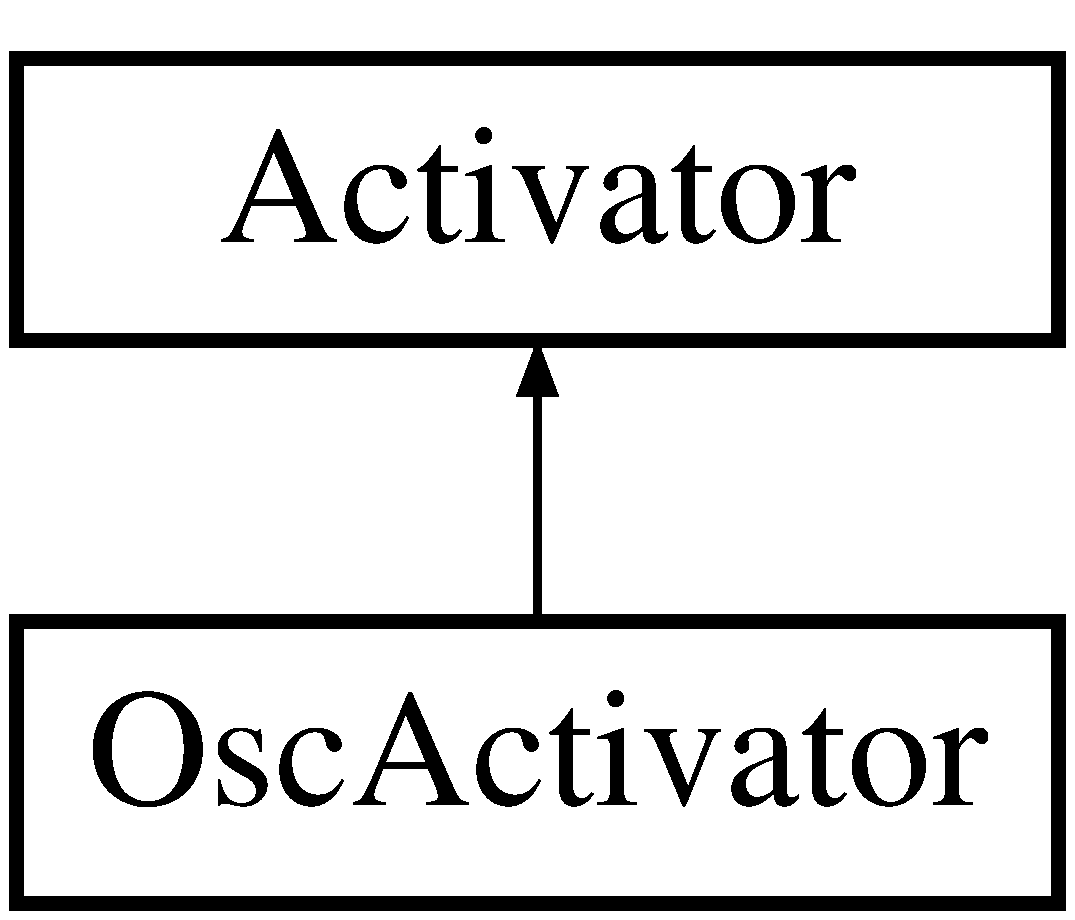
\includegraphics[height=2.000000cm]{classActivator}
\end{center}
\end{figure}
\subsection*{Public Member Functions}
\begin{DoxyCompactItemize}
\item 
virtual void {\bfseries callback} (float value)\hypertarget{classActivator_ace74b175ffcc2ad9cc03f15a0e713743}{}\label{classActivator_ace74b175ffcc2ad9cc03f15a0e713743}

\end{DoxyCompactItemize}


The documentation for this class was generated from the following files\+:\begin{DoxyCompactItemize}
\item 
include/Activator.\+h\item 
sequencer/Activator.\+cpp\end{DoxyCompactItemize}

\hypertarget{classunit_1_1AddTwoGen}{}\section{unit\+:\+:Add\+Two\+Gen Class Reference}
\label{classunit_1_1AddTwoGen}\index{unit\+::\+Add\+Two\+Gen@{unit\+::\+Add\+Two\+Gen}}


{\ttfamily \#include $<$Add\+Two\+Gen.\+h$>$}

Inheritance diagram for unit\+:\+:Add\+Two\+Gen\+:\begin{figure}[H]
\begin{center}
\leavevmode
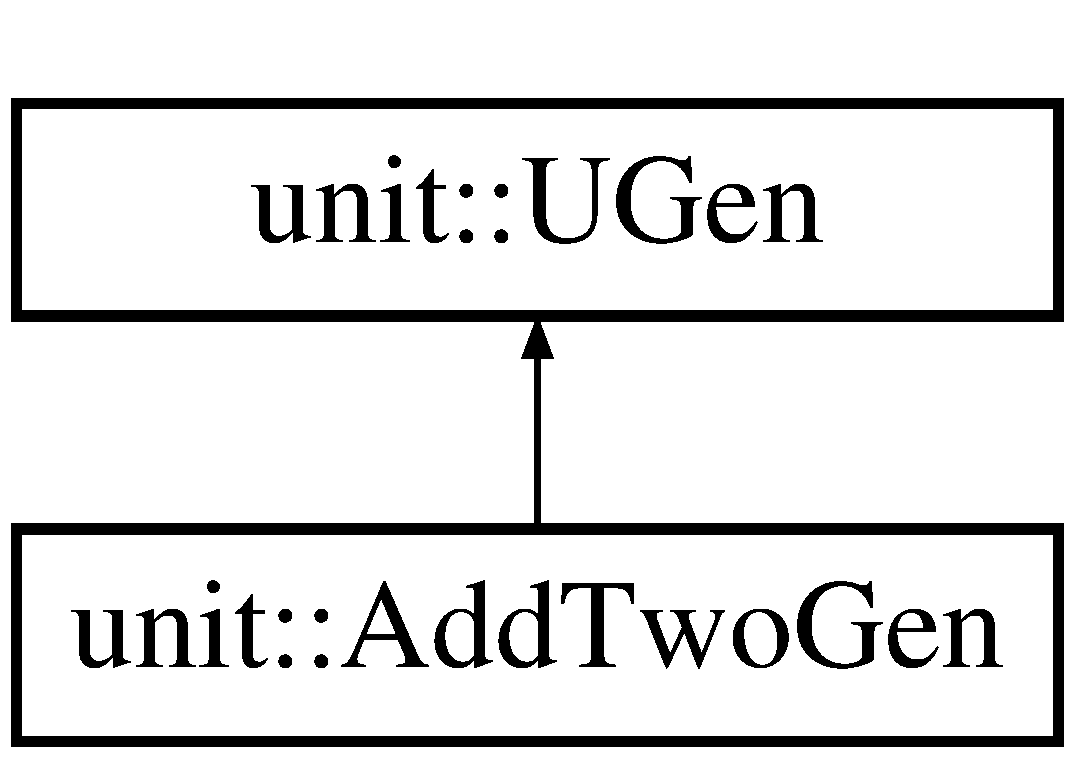
\includegraphics[height=2.000000cm]{classunit_1_1AddTwoGen}
\end{center}
\end{figure}
\subsection*{Public Member Functions}
\begin{DoxyCompactItemize}
\item 
{\bfseries Add\+Two\+Gen} (std\+::string name)\hypertarget{classunit_1_1AddTwoGen_a6feb4da948f12b37eb4502899b5a4311}{}\label{classunit_1_1AddTwoGen_a6feb4da948f12b37eb4502899b5a4311}

\item 
void {\bfseries control} (std\+::string port\+Name, float value)\hypertarget{classunit_1_1AddTwoGen_a5e0a82722566595b7284386a618ef3cb}{}\label{classunit_1_1AddTwoGen_a5e0a82722566595b7284386a618ef3cb}

\item 
float {\bfseries tick} ()\hypertarget{classunit_1_1AddTwoGen_a8e667f4f6c6849faef9f07a62e779d9a}{}\label{classunit_1_1AddTwoGen_a8e667f4f6c6849faef9f07a62e779d9a}

\end{DoxyCompactItemize}
\subsection*{Additional Inherited Members}


\subsection{Detailed Description}
\hyperlink{classunit_1_1AddTwoGen}{Add\+Two\+Gen} is calculating the arithmetic mean of \hyperlink{classPort}{Port} in1 and \hyperlink{classPort}{Port} in2. It provides a very basic two input mixing unit, adding together the Ports in1 and in2.

\begin{DoxyAuthor}{Author}
jtm 
\end{DoxyAuthor}
\begin{DoxySince}{Since}
04-\/2016 
\end{DoxySince}
\begin{DoxyVersion}{Version}
1.\+0 
\end{DoxyVersion}


The documentation for this class was generated from the following files\+:\begin{DoxyCompactItemize}
\item 
include/Add\+Two\+Gen.\+h\item 
unit/Add\+Two\+Gen.\+cpp\end{DoxyCompactItemize}

\hypertarget{classunit_1_1ADSRGen}{\section{unit\-:\-:A\-D\-S\-R\-Gen Class Reference}
\label{classunit_1_1ADSRGen}\index{unit\-::\-A\-D\-S\-R\-Gen@{unit\-::\-A\-D\-S\-R\-Gen}}
}
Inheritance diagram for unit\-:\-:A\-D\-S\-R\-Gen\-:\begin{figure}[H]
\begin{center}
\leavevmode
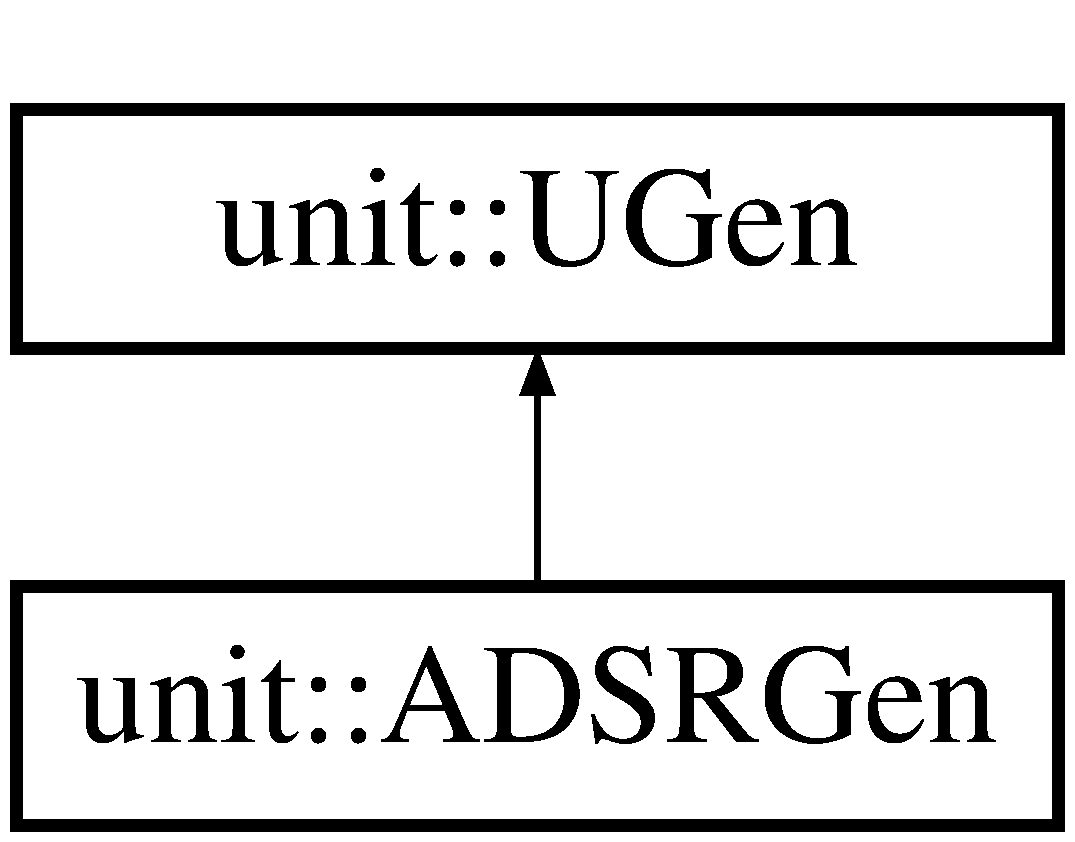
\includegraphics[height=3.000000cm]{classunit_1_1ADSRGen}
\end{center}
\end{figure}
\subsection*{Public Member Functions}
\begin{DoxyCompactItemize}
\item 
\hypertarget{classunit_1_1ADSRGen_a7e2d63eecbe51fc86a93697dd4d47964}{{\bfseries A\-D\-S\-R\-Gen} (std\-::string name)}\label{classunit_1_1ADSRGen_a7e2d63eecbe51fc86a93697dd4d47964}

\item 
\hypertarget{classunit_1_1ADSRGen_ac43bddd25b9a84f0ad6b299ed55f5133}{void {\bfseries control} (std\-::string port\-Name, float value)}\label{classunit_1_1ADSRGen_ac43bddd25b9a84f0ad6b299ed55f5133}

\item 
\hypertarget{classunit_1_1ADSRGen_a91a149fa5065d94dccec224b18710a24}{float {\bfseries tick} ()}\label{classunit_1_1ADSRGen_a91a149fa5065d94dccec224b18710a24}

\item 
\hypertarget{classunit_1_1ADSRGen_a8685be5cffea6ec29dc1ebdc44402f70}{void {\bfseries set\-Trigger} ()}\label{classunit_1_1ADSRGen_a8685be5cffea6ec29dc1ebdc44402f70}

\item 
\hypertarget{classunit_1_1ADSRGen_aee81e429433522eeb6362338fe15d551}{void {\bfseries set\-Gate} (float value)}\label{classunit_1_1ADSRGen_aee81e429433522eeb6362338fe15d551}

\item 
\hypertarget{classunit_1_1ADSRGen_a3a81f7181fa8b63f4ec5ff9da91cb8b3}{void {\bfseries set\-Attack} (float value)}\label{classunit_1_1ADSRGen_a3a81f7181fa8b63f4ec5ff9da91cb8b3}

\item 
\hypertarget{classunit_1_1ADSRGen_a14856bf0586881cbe088ab47918b7d72}{void {\bfseries set\-Decay} (float value)}\label{classunit_1_1ADSRGen_a14856bf0586881cbe088ab47918b7d72}

\item 
\hypertarget{classunit_1_1ADSRGen_a07fa6e650dc1ffdde91fc0721d4a8dc8}{void {\bfseries set\-Sustain} (float value)}\label{classunit_1_1ADSRGen_a07fa6e650dc1ffdde91fc0721d4a8dc8}

\item 
\hypertarget{classunit_1_1ADSRGen_a8c2a3e60dcae34d077b5983b1584de71}{void {\bfseries set\-Release} (float value)}\label{classunit_1_1ADSRGen_a8c2a3e60dcae34d077b5983b1584de71}

\end{DoxyCompactItemize}
\subsection*{Additional Inherited Members}


The documentation for this class was generated from the following files\-:\begin{DoxyCompactItemize}
\item 
include/A\-D\-S\-R\-Gen.\-h\item 
unit/A\-D\-S\-R\-Gen.\-cpp\end{DoxyCompactItemize}

\hypertarget{classCentralStore}{\section{Central\-Store Class Reference}
\label{classCentralStore}\index{Central\-Store@{Central\-Store}}
}
\subsection*{Public Member Functions}
\begin{DoxyCompactItemize}
\item 
\hypertarget{classCentralStore_ab809e0f4e90d4d8d1873a89f3da889b3}{void {\bfseries tick} ()}\label{classCentralStore_ab809e0f4e90d4d8d1873a89f3da889b3}

\item 
\hypertarget{classCentralStore_a100ae6ad2506d4962d23966e23a1c78e}{void {\bfseries clear} ()}\label{classCentralStore_a100ae6ad2506d4962d23966e23a1c78e}

\item 
\hypertarget{classCentralStore_a910470f5eec98b92b82a4cb2f1c5f386}{\hyperlink{classosc_1_1MessageData}{osc\-::\-Message\-Data} $\ast$ {\bfseries get\-Midi\-Data} ()}\label{classCentralStore_a910470f5eec98b92b82a4cb2f1c5f386}

\item 
\hypertarget{classCentralStore_a3faaea58a012d25efaa710fa3d1942b7}{\hyperlink{classosc_1_1MessageData}{osc\-::\-Message\-Data} $\ast$ {\bfseries get\-Control\-Data} ()}\label{classCentralStore_a3faaea58a012d25efaa710fa3d1942b7}

\end{DoxyCompactItemize}
\subsection*{Public Attributes}
\begin{DoxyCompactItemize}
\item 
\hypertarget{classCentralStore_a6f0c4050f0983924bbad8c631746f8b7}{\hyperlink{structTickData}{Tick\-Data} {\bfseries tick\-Data}}\label{classCentralStore_a6f0c4050f0983924bbad8c631746f8b7}

\end{DoxyCompactItemize}


The documentation for this class was generated from the following files\-:\begin{DoxyCompactItemize}
\item 
src/include/Central\-Store.\-h\item 
src/store/Central\-Store.\-cpp\end{DoxyCompactItemize}

\hypertarget{classConfigurationManager}{}\section{Configuration\+Manager Class Reference}
\label{classConfigurationManager}\index{Configuration\+Manager@{Configuration\+Manager}}
\subsection*{Public Member Functions}
\begin{DoxyCompactItemize}
\item 
void {\bfseries load} (std\+::string fname)\hypertarget{classConfigurationManager_a066a7ae7e01b7ba6b62782fd3eeffaab}{}\label{classConfigurationManager_a066a7ae7e01b7ba6b62782fd3eeffaab}

\item 
std\+::string {\bfseries get\+Working\+Path} ()\hypertarget{classConfigurationManager_ab4fac4121f154fb83b67a727b650c436}{}\label{classConfigurationManager_ab4fac4121f154fb83b67a727b650c436}

\end{DoxyCompactItemize}


The documentation for this class was generated from the following files\+:\begin{DoxyCompactItemize}
\item 
include/Configuration\+Manager.\+h\item 
configuration/Configuration\+Manager.\+cpp\end{DoxyCompactItemize}

\hypertarget{classConsumerThread}{\section{Consumer\-Thread Class Reference}
\label{classConsumerThread}\index{Consumer\-Thread@{Consumer\-Thread}}
}
Inheritance diagram for Consumer\-Thread\-:\begin{figure}[H]
\begin{center}
\leavevmode
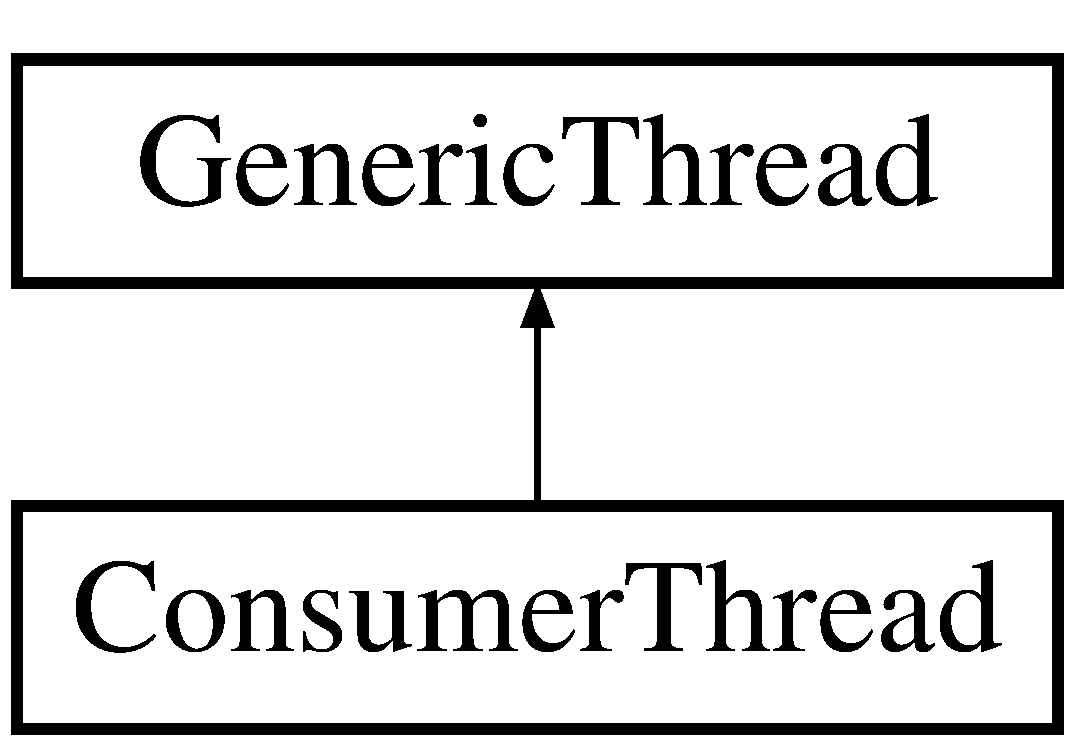
\includegraphics[height=2.000000cm]{classConsumerThread}
\end{center}
\end{figure}
\subsection*{Public Member Functions}
\begin{DoxyCompactItemize}
\item 
\hypertarget{classConsumerThread_a000214667d1ad9d31ce7133f6fbf9aac}{{\bfseries Consumer\-Thread} (\hyperlink{classGenericQueue}{Generic\-Queue}$<$ \hyperlink{classWorkItem}{Work\-Item} $\ast$ $>$ \&queue)}\label{classConsumerThread_a000214667d1ad9d31ce7133f6fbf9aac}

\item 
\hypertarget{classConsumerThread_a8fde7a9b6c2c0b3c62a9fd3c50296557}{void $\ast$ {\bfseries run} ()}\label{classConsumerThread_a8fde7a9b6c2c0b3c62a9fd3c50296557}

\end{DoxyCompactItemize}


The documentation for this class was generated from the following file\-:\begin{DoxyCompactItemize}
\item 
src/store/gqueue.\-cpp\end{DoxyCompactItemize}

\hypertarget{classunit_1_1EGOneStepGen}{\section{unit\-:\-:E\-G\-One\-Step\-Gen Class Reference}
\label{classunit_1_1EGOneStepGen}\index{unit\-::\-E\-G\-One\-Step\-Gen@{unit\-::\-E\-G\-One\-Step\-Gen}}
}


{\ttfamily \#include $<$E\-G\-One\-Step\-Gen.\-h$>$}

Inheritance diagram for unit\-:\-:E\-G\-One\-Step\-Gen\-:\begin{figure}[H]
\begin{center}
\leavevmode
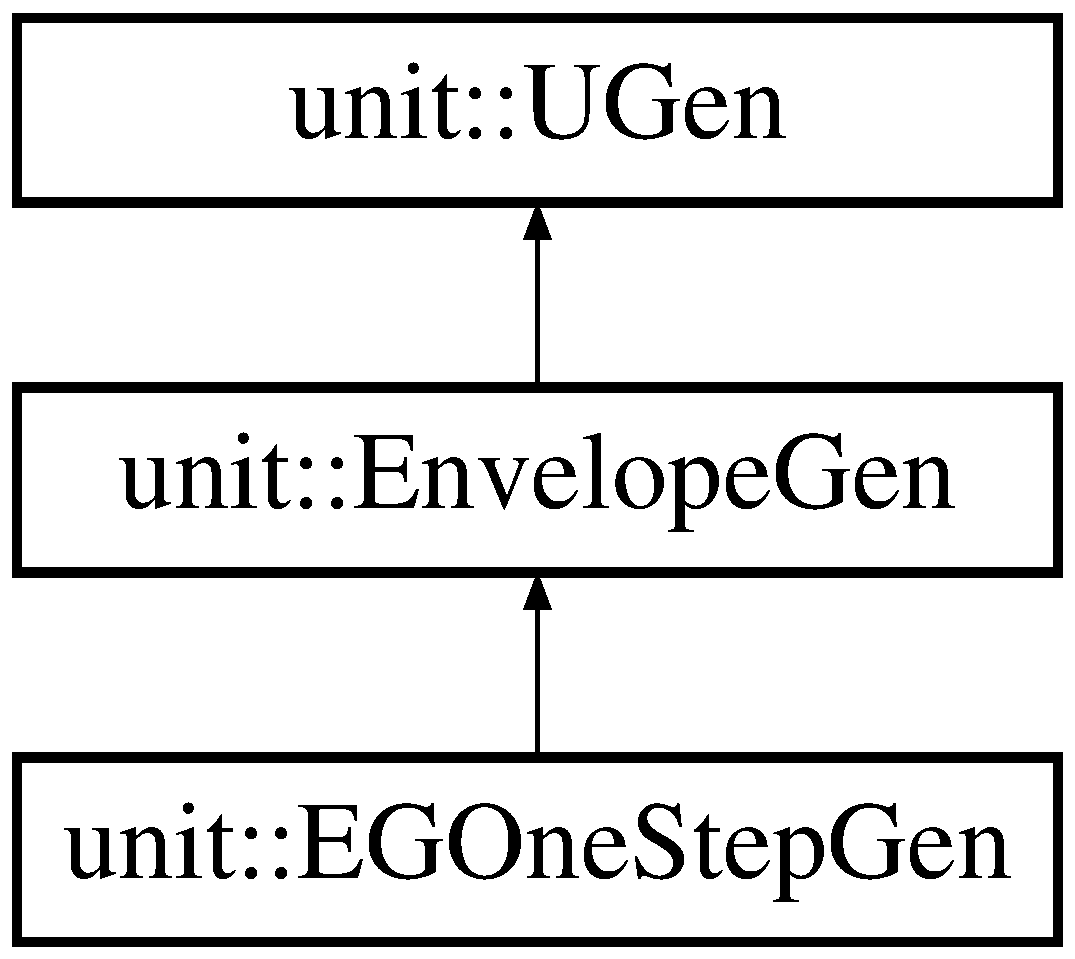
\includegraphics[height=3.000000cm]{classunit_1_1EGOneStepGen}
\end{center}
\end{figure}
\subsection*{Public Member Functions}
\begin{DoxyCompactItemize}
\item 
\hypertarget{classunit_1_1EGOneStepGen_a9bc697acabed6c7b0467369ba073ede1}{{\bfseries E\-G\-One\-Step\-Gen} (std\-::string name)}\label{classunit_1_1EGOneStepGen_a9bc697acabed6c7b0467369ba073ede1}

\item 
\hypertarget{classunit_1_1EGOneStepGen_a74df96649d7a66d19cb33bf9bf13f54a}{float {\bfseries tick} ()}\label{classunit_1_1EGOneStepGen_a74df96649d7a66d19cb33bf9bf13f54a}

\item 
\hypertarget{classunit_1_1EGOneStepGen_a8979594fb226c732a9b8232664f09047}{void {\bfseries control} (std\-::string port\-Name, float value)}\label{classunit_1_1EGOneStepGen_a8979594fb226c732a9b8232664f09047}

\item 
\hypertarget{classunit_1_1EGOneStepGen_ae9f187e0f266559a80e4f4b534d79f78}{bool {\bfseries finished} ()}\label{classunit_1_1EGOneStepGen_ae9f187e0f266559a80e4f4b534d79f78}

\item 
\hypertarget{classunit_1_1EGOneStepGen_af94a0976e166a3f53b7bf14de58f81d6}{void {\bfseries set\-Trigger} ()}\label{classunit_1_1EGOneStepGen_af94a0976e166a3f53b7bf14de58f81d6}

\item 
\hypertarget{classunit_1_1EGOneStepGen_aaf02138e168cad06cb955944f57ce93c}{void {\bfseries set\-Duration} (float seconds)}\label{classunit_1_1EGOneStepGen_aaf02138e168cad06cb955944f57ce93c}

\item 
\hypertarget{classunit_1_1EGOneStepGen_af2b5bd8522fac9dc997d78d3750cdbbb}{void {\bfseries set\-Start\-Level} (float level)}\label{classunit_1_1EGOneStepGen_af2b5bd8522fac9dc997d78d3750cdbbb}

\item 
\hypertarget{classunit_1_1EGOneStepGen_a3d58403aa5bebffeaf3f326855e0a233}{void {\bfseries set\-End\-Level} (float level)}\label{classunit_1_1EGOneStepGen_a3d58403aa5bebffeaf3f326855e0a233}

\item 
\hypertarget{classunit_1_1EGOneStepGen_a4898b08a0687e03802abdb7945708cab}{void {\bfseries reset} ()}\label{classunit_1_1EGOneStepGen_a4898b08a0687e03802abdb7945708cab}

\end{DoxyCompactItemize}
\subsection*{Additional Inherited Members}


\subsection{Detailed Description}
\hyperlink{classunit_1_1EGOneStepGen}{E\-G\-One\-Step\-Gen} is providing a linear interpolation based on the current time step.

\begin{DoxyAuthor}{Author}
jtm 
\end{DoxyAuthor}
\begin{DoxySince}{Since}
04-\/2016 
\end{DoxySince}
\begin{DoxyVersion}{Version}
1.\-0 
\end{DoxyVersion}


The documentation for this class was generated from the following files\-:\begin{DoxyCompactItemize}
\item 
src/include/E\-G\-One\-Step\-Gen.\-h\item 
src/unit/E\-G\-One\-Step\-Gen.\-cpp\end{DoxyCompactItemize}

\hypertarget{classunit_1_1EGUpDownGen}{}\section{unit\+:\+:E\+G\+Up\+Down\+Gen Class Reference}
\label{classunit_1_1EGUpDownGen}\index{unit\+::\+E\+G\+Up\+Down\+Gen@{unit\+::\+E\+G\+Up\+Down\+Gen}}


{\ttfamily \#include $<$E\+G\+Up\+Down\+Gen.\+h$>$}

Inheritance diagram for unit\+:\+:E\+G\+Up\+Down\+Gen\+:\begin{figure}[H]
\begin{center}
\leavevmode
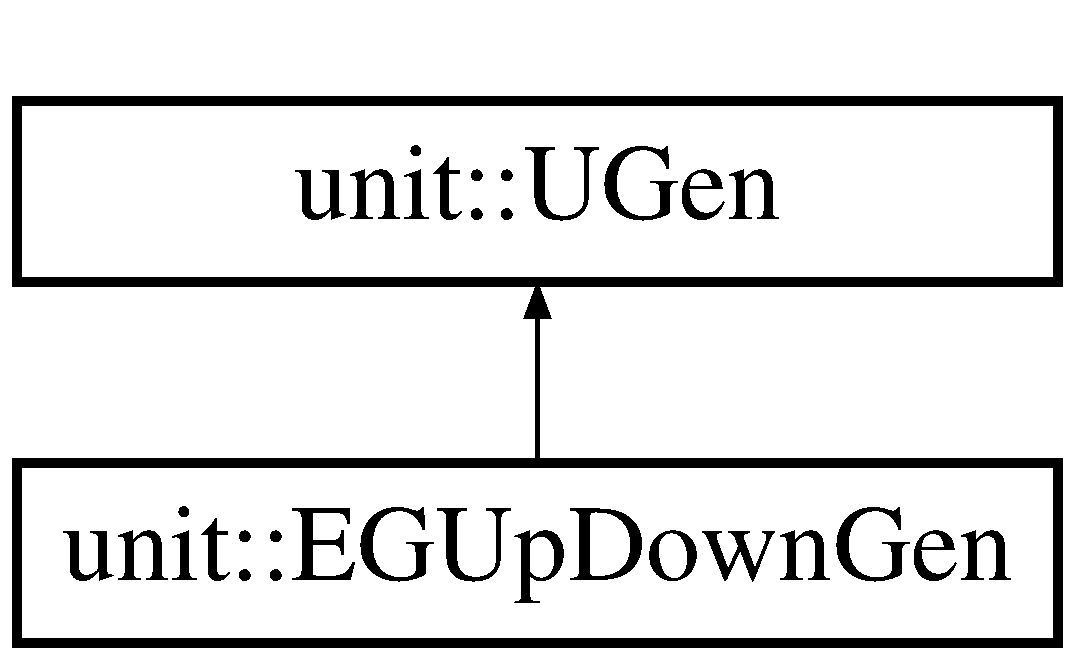
\includegraphics[height=3.000000cm]{classunit_1_1EGUpDownGen}
\end{center}
\end{figure}
\subsection*{Public Member Functions}
\begin{DoxyCompactItemize}
\item 
{\bfseries E\+G\+Up\+Down\+Gen} (std\+::string name)\hypertarget{classunit_1_1EGUpDownGen_abc35a572da36fa26f4b54beabfc6268e}{}\label{classunit_1_1EGUpDownGen_abc35a572da36fa26f4b54beabfc6268e}

\item 
float {\bfseries tick} ()\hypertarget{classunit_1_1EGUpDownGen_abea11de5389345064a8395d54411e3b3}{}\label{classunit_1_1EGUpDownGen_abea11de5389345064a8395d54411e3b3}

\item 
void {\bfseries control} (std\+::string port\+Name, float value)\hypertarget{classunit_1_1EGUpDownGen_ac1ef59d9023034c17b46e09bfae15178}{}\label{classunit_1_1EGUpDownGen_ac1ef59d9023034c17b46e09bfae15178}

\end{DoxyCompactItemize}
\subsection*{Additional Inherited Members}


\subsection{Detailed Description}
\hyperlink{classunit_1_1EGUpDownGen}{E\+G\+Up\+Down\+Gen} generates a simple symetrical up/down envelope.

\begin{DoxyAuthor}{Author}
jtm, email\+:  \href{mailto:milde@hs-fulda.de}{\tt milde@hs-\/fulda.\+de} 
\end{DoxyAuthor}
\begin{DoxySince}{Since}
04-\/2016 
\end{DoxySince}
\begin{DoxyVersion}{Version}
1.\+0 
\end{DoxyVersion}


The documentation for this class was generated from the following files\+:\begin{DoxyCompactItemize}
\item 
include/E\+G\+Up\+Down\+Gen.\+h\item 
unit/E\+G\+Up\+Down\+Gen.\+cpp\end{DoxyCompactItemize}

\hypertarget{classExamplePacketListener}{}\section{Example\+Packet\+Listener Class Reference}
\label{classExamplePacketListener}\index{Example\+Packet\+Listener@{Example\+Packet\+Listener}}
Inheritance diagram for Example\+Packet\+Listener\+:\begin{figure}[H]
\begin{center}
\leavevmode
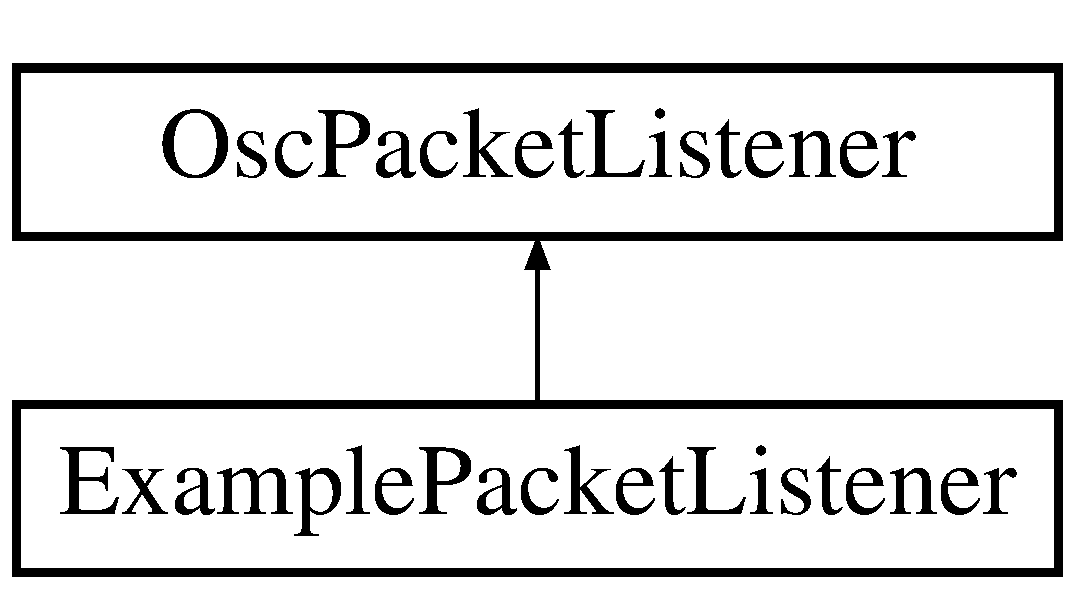
\includegraphics[height=2.000000cm]{classExamplePacketListener}
\end{center}
\end{figure}
\subsection*{Protected Member Functions}
\begin{DoxyCompactItemize}
\item 
virtual void {\bfseries Process\+Message} (const osc\+::\+Received\+Message \&m, const Ip\+Endpoint\+Name \&remote\+Endpoint)\hypertarget{classExamplePacketListener_a688ed2a3ec01d0fb7661f4fe0ffc90df}{}\label{classExamplePacketListener_a688ed2a3ec01d0fb7661f4fe0ffc90df}

\end{DoxyCompactItemize}


The documentation for this class was generated from the following file\+:\begin{DoxyCompactItemize}
\item 
Simple\+Receive.\+cpp\end{DoxyCompactItemize}

\hypertarget{classunit_1_1GatedConstantGen}{}\section{unit\+:\+:Gated\+Constant\+Gen Class Reference}
\label{classunit_1_1GatedConstantGen}\index{unit\+::\+Gated\+Constant\+Gen@{unit\+::\+Gated\+Constant\+Gen}}
Inheritance diagram for unit\+:\+:Gated\+Constant\+Gen\+:\begin{figure}[H]
\begin{center}
\leavevmode
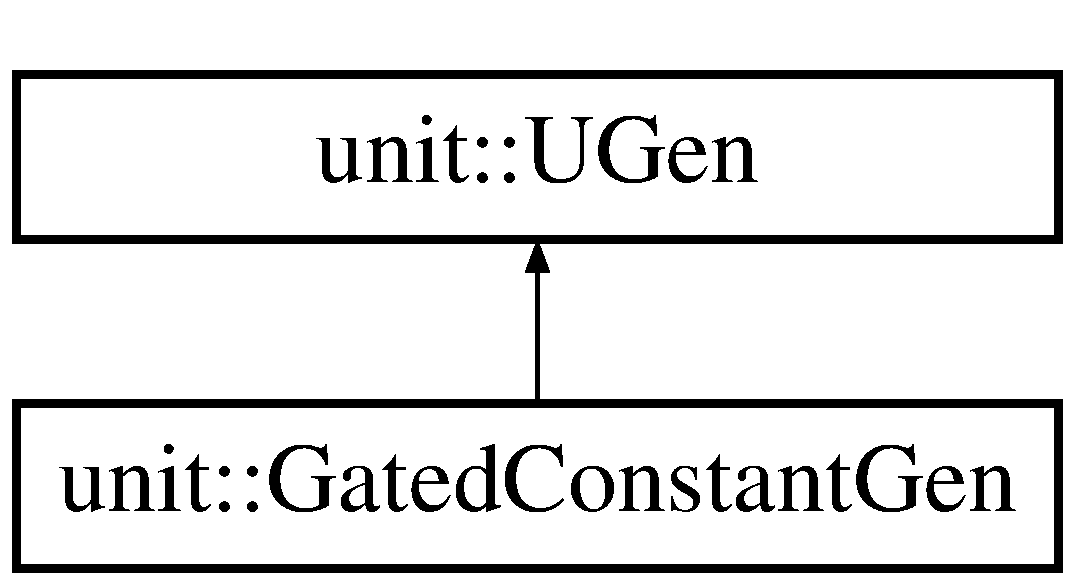
\includegraphics[height=2.000000cm]{classunit_1_1GatedConstantGen}
\end{center}
\end{figure}
\subsection*{Public Member Functions}
\begin{DoxyCompactItemize}
\item 
{\bfseries Gated\+Constant\+Gen} (std\+::string name)\hypertarget{classunit_1_1GatedConstantGen_ad30ad26411f421228c8f7075b4d27f9a}{}\label{classunit_1_1GatedConstantGen_ad30ad26411f421228c8f7075b4d27f9a}

\item 
void {\bfseries control} (std\+::string port\+Name, float value)\hypertarget{classunit_1_1GatedConstantGen_a8365ddc2a6ddebc86e196fa381a5648d}{}\label{classunit_1_1GatedConstantGen_a8365ddc2a6ddebc86e196fa381a5648d}

\item 
float {\bfseries tick} ()\hypertarget{classunit_1_1GatedConstantGen_aafff659359fed9f28c703acd0076c081}{}\label{classunit_1_1GatedConstantGen_aafff659359fed9f28c703acd0076c081}

\end{DoxyCompactItemize}
\subsection*{Additional Inherited Members}


The documentation for this class was generated from the following files\+:\begin{DoxyCompactItemize}
\item 
unit/Gated\+Constant\+Gen.\+h\item 
unit/Gated\+Constant\+Gen.\+cpp\end{DoxyCompactItemize}

\hypertarget{classGenericQueue}{\section{Generic\-Queue$<$ T $>$ Class Template Reference}
\label{classGenericQueue}\index{Generic\-Queue$<$ T $>$@{Generic\-Queue$<$ T $>$}}
}
\subsection*{Public Member Functions}
\begin{DoxyCompactItemize}
\item 
\hypertarget{classGenericQueue_af5de20e93f3ee8d1fdd38a8ec1ae52f6}{void {\bfseries add} (T item)}\label{classGenericQueue_af5de20e93f3ee8d1fdd38a8ec1ae52f6}

\item 
\hypertarget{classGenericQueue_a15366cdc3234d238c664c82524f14c0b}{T {\bfseries remove} ()}\label{classGenericQueue_a15366cdc3234d238c664c82524f14c0b}

\item 
\hypertarget{classGenericQueue_aa94c712ca621ef5c121cd4f9c9188f67}{int {\bfseries size} ()}\label{classGenericQueue_aa94c712ca621ef5c121cd4f9c9188f67}

\item 
\hypertarget{classGenericQueue_a0fd02ceeecaf5c0903e3ee7199b183bc}{void {\bfseries clear} ()}\label{classGenericQueue_a0fd02ceeecaf5c0903e3ee7199b183bc}

\end{DoxyCompactItemize}


The documentation for this class was generated from the following file\-:\begin{DoxyCompactItemize}
\item 
src/include/Generic\-Queue.\-h\end{DoxyCompactItemize}

\hypertarget{classGenericThread}{}\section{Generic\+Thread Class Reference}
\label{classGenericThread}\index{Generic\+Thread@{Generic\+Thread}}
Inheritance diagram for Generic\+Thread\+:\begin{figure}[H]
\begin{center}
\leavevmode
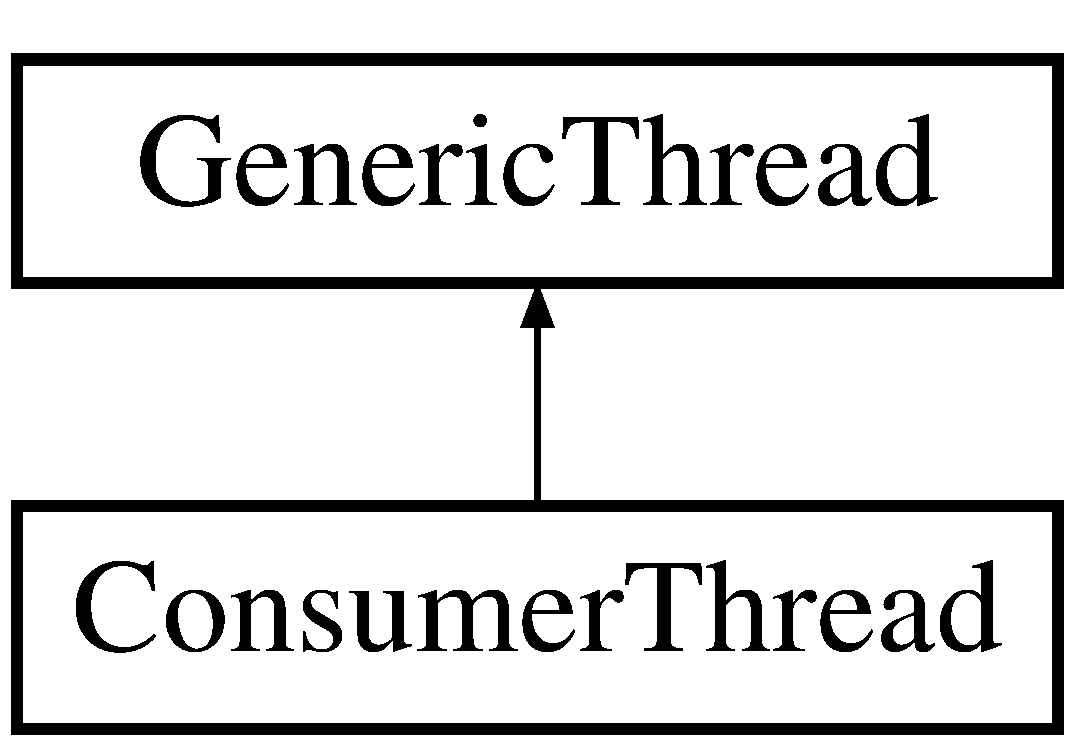
\includegraphics[height=2.000000cm]{classGenericThread}
\end{center}
\end{figure}
\subsection*{Public Member Functions}
\begin{DoxyCompactItemize}
\item 
int {\bfseries start} ()\hypertarget{classGenericThread_ac1d8c3d7dcaae01e89c69093a065141f}{}\label{classGenericThread_ac1d8c3d7dcaae01e89c69093a065141f}

\item 
int {\bfseries join} ()\hypertarget{classGenericThread_a217ef41077ae00ce48372c03838af96a}{}\label{classGenericThread_a217ef41077ae00ce48372c03838af96a}

\item 
int {\bfseries detach} ()\hypertarget{classGenericThread_abd0849015ec4004b789aa3181853fbf6}{}\label{classGenericThread_abd0849015ec4004b789aa3181853fbf6}

\item 
pthread\+\_\+t {\bfseries self} ()\hypertarget{classGenericThread_a0ac1c8aa0c6f5d47d73626c13854d444}{}\label{classGenericThread_a0ac1c8aa0c6f5d47d73626c13854d444}

\item 
virtual void $\ast$ {\bfseries run} ()=0\hypertarget{classGenericThread_a54147ff9f16e7985e634b5f0d6d5b7f9}{}\label{classGenericThread_a54147ff9f16e7985e634b5f0d6d5b7f9}

\end{DoxyCompactItemize}


The documentation for this class was generated from the following files\+:\begin{DoxyCompactItemize}
\item 
store/Generic\+Thread.\+h\item 
store/Generic\+Thread.\+cpp\end{DoxyCompactItemize}

\hypertarget{classIDGenerator}{\section{I\-D\-Generator Class Reference}
\label{classIDGenerator}\index{I\-D\-Generator@{I\-D\-Generator}}
}
\subsection*{Public Member Functions}
\begin{DoxyCompactItemize}
\item 
\hypertarget{classIDGenerator_a223bf057a0ad9e69df527142dfe1e91b}{std\-::string {\bfseries next\-I\-D} ()}\label{classIDGenerator_a223bf057a0ad9e69df527142dfe1e91b}

\end{DoxyCompactItemize}


The documentation for this class was generated from the following files\-:\begin{DoxyCompactItemize}
\item 
include/I\-D\-Generator.\-h\item 
util/I\-D\-Generator.\-cpp\end{DoxyCompactItemize}

\hypertarget{classInterpolation}{}\section{Interpolation Class Reference}
\label{classInterpolation}\index{Interpolation@{Interpolation}}


{\ttfamily \#include $<$Interpolation.\+h$>$}

\subsection*{Static Public Member Functions}
\begin{DoxyCompactItemize}
\item 
static float {\bfseries map} (float value, float s1, float e1, float s2, float e2)\hypertarget{classInterpolation_adfd3003c39c40ec76342274c65017761}{}\label{classInterpolation_adfd3003c39c40ec76342274c65017761}

\item 
static float {\bfseries map} (int value, int s1, int e1, float s2, float e2)\hypertarget{classInterpolation_ac6eab12deb9f79b79200aad3b219e7c3}{}\label{classInterpolation_ac6eab12deb9f79b79200aad3b219e7c3}

\item 
static int {\bfseries discrete} (float value, float s1, float e1, int max)\hypertarget{classInterpolation_a246c72a835822b7674758d657ed44230}{}\label{classInterpolation_a246c72a835822b7674758d657ed44230}

\item 
static float \hyperlink{classInterpolation_a5549f8859f14153da891222a8ff1a22f}{maplog} (float value, float s1, float e1, float s2, float e2)
\item 
static float {\bfseries mapexp} (float value, float s1, float e1, float s2, float e2)\hypertarget{classInterpolation_a08d1fe5e82708ab26a019e9ae9f851c8}{}\label{classInterpolation_a08d1fe5e82708ab26a019e9ae9f851c8}

\end{DoxyCompactItemize}


\subsection{Detailed Description}
\hyperlink{classInterpolation}{Interpolation} provides a number of helper function to easily calculate the linear interpolation of a value.

\begin{DoxyAuthor}{Author}
jtm 
\end{DoxyAuthor}
\begin{DoxySince}{Since}
04-\/2016 
\end{DoxySince}
\begin{DoxyVersion}{Version}
1.\+0 
\end{DoxyVersion}


\subsection{Member Function Documentation}
\index{Interpolation@{Interpolation}!maplog@{maplog}}
\index{maplog@{maplog}!Interpolation@{Interpolation}}
\subsubsection[{\texorpdfstring{maplog(float value, float s1, float e1, float s2, float e2)}{maplog(float value, float s1, float e1, float s2, float e2)}}]{\setlength{\rightskip}{0pt plus 5cm}float Interpolation\+::maplog (
\begin{DoxyParamCaption}
\item[{float}]{value, }
\item[{float}]{s1, }
\item[{float}]{e1, }
\item[{float}]{s2, }
\item[{float}]{e2}
\end{DoxyParamCaption}
)\hspace{0.3cm}{\ttfamily [static]}}\hypertarget{classInterpolation_a5549f8859f14153da891222a8ff1a22f}{}\label{classInterpolation_a5549f8859f14153da891222a8ff1a22f}
Calculates the logarithm() of the linear mapping of the input value from interval \mbox{[}s1,e1\mbox{]} to interval \mbox{[}s2,e2\mbox{]}.


\begin{DoxyItemize}
\item The logarithmic result allows for a more fine grained control of the {\bfseries higher} end of the interval.
\item The result should be normalized by dividing the result by log(e2-\/s2).
\end{DoxyItemize}

\begin{DoxyReturn}{Returns}
The log() of the linear mapping.
\end{DoxyReturn}

\begin{DoxyParams}{Parameters}
{\em value} & the value to be mapped (e.\+g. a knob value) \\
\hline
{\em s1} & start of domain interval \\
\hline
{\em e1} & end of domain interval \\
\hline
{\em s2} & start of range interval \\
\hline
{\em e2} & end of range interval \\
\hline
\end{DoxyParams}


The documentation for this class was generated from the following files\+:\begin{DoxyCompactItemize}
\item 
include/Interpolation.\+h\item 
util/Interpolation.\+cpp\end{DoxyCompactItemize}

\hypertarget{classMessageData}{}\section{Message\+Data Class Reference}
\label{classMessageData}\index{Message\+Data@{Message\+Data}}
\subsection*{Public Types}
\begin{DoxyCompactItemize}
\item 
enum {\bfseries Types} \{ \\*
{\bfseries M\+I\+D\+I\+ON}, 
{\bfseries M\+I\+D\+I\+O\+FF}, 
{\bfseries C\+O\+N\+T\+R\+OL}, 
{\bfseries P\+A\+D\+ON}, 
\\*
{\bfseries P\+A\+D\+O\+FF}, 
{\bfseries S\+L\+I\+D\+ER}, 
{\bfseries U\+N\+K\+N\+O\+WN}
 \}\hypertarget{classMessageData_a63f99930873414c0908b5e735964e022}{}\label{classMessageData_a63f99930873414c0908b5e735964e022}

\end{DoxyCompactItemize}
\subsection*{Public Member Functions}
\begin{DoxyCompactItemize}
\item 
{\bfseries Message\+Data} (std\+::string s, int a1, int a2, int a3, float f)\hypertarget{classMessageData_af370333b9828ad63ba1031ac941300c2}{}\label{classMessageData_af370333b9828ad63ba1031ac941300c2}

\item 
{\bfseries Message\+Data} (\hyperlink{classMessageData}{Message\+Data} $\ast$md)\hypertarget{classMessageData_acf5694351e2f877340d6b38044d8b2d3}{}\label{classMessageData_acf5694351e2f877340d6b38044d8b2d3}

\item 
std\+::string {\bfseries get\+Message} ()\hypertarget{classMessageData_a8bf658a5be5789142fa260512fded9a1}{}\label{classMessageData_a8bf658a5be5789142fa260512fded9a1}

\item 
int {\bfseries get\+Code} ()\hypertarget{classMessageData_aa625a45bf78b8351d29a7696c8f014e9}{}\label{classMessageData_aa625a45bf78b8351d29a7696c8f014e9}

\item 
int {\bfseries get\+Key} ()\hypertarget{classMessageData_ab70773361a5ffba488a83b0d87cfb25c}{}\label{classMessageData_ab70773361a5ffba488a83b0d87cfb25c}

\item 
int {\bfseries get\+Value} ()\hypertarget{classMessageData_af79bf248fbb542bd25984f7f2b3993eb}{}\label{classMessageData_af79bf248fbb542bd25984f7f2b3993eb}

\item 
float {\bfseries get\+F1} ()\hypertarget{classMessageData_ad1e951e980e59c5d222b79856cae6d32}{}\label{classMessageData_ad1e951e980e59c5d222b79856cae6d32}

\item 
Types {\bfseries get\+Type} ()\hypertarget{classMessageData_a38c69b7ebcf46e7c19ff2409af36a7ae}{}\label{classMessageData_a38c69b7ebcf46e7c19ff2409af36a7ae}

\item 
void {\bfseries set\+Message} (std\+::string s)\hypertarget{classMessageData_a1da8f45a1453c7d11029fa360d7a642c}{}\label{classMessageData_a1da8f45a1453c7d11029fa360d7a642c}

\item 
void {\bfseries adapt\+Message\+Type} ()\hypertarget{classMessageData_a0f8ce5f6d5c4452e26656236ee7aefc3}{}\label{classMessageData_a0f8ce5f6d5c4452e26656236ee7aefc3}

\item 
void {\bfseries set\+Code} (int a1)\hypertarget{classMessageData_a8639583a844208ccae9568bb68d1e547}{}\label{classMessageData_a8639583a844208ccae9568bb68d1e547}

\item 
void {\bfseries set\+Key} (int a2)\hypertarget{classMessageData_a54a0ddfb44fba671ba243914b037e231}{}\label{classMessageData_a54a0ddfb44fba671ba243914b037e231}

\item 
void {\bfseries set\+Value} (int a3)\hypertarget{classMessageData_a24e273f0a4443505ccf6222405cfb567}{}\label{classMessageData_a24e273f0a4443505ccf6222405cfb567}

\item 
void {\bfseries set\+F1} (float f)\hypertarget{classMessageData_a94dce06ace95a93c075dbaf253e559fe}{}\label{classMessageData_a94dce06ace95a93c075dbaf253e559fe}

\item 
void {\bfseries set\+Message\+Data} (std\+::string s, int a1, int a2, int a3, float f)\hypertarget{classMessageData_a9eb7741e4216075b0e03c554d83e35ae}{}\label{classMessageData_a9eb7741e4216075b0e03c554d83e35ae}

\item 
bool {\bfseries is\+Fresh} ()\hypertarget{classMessageData_a169f4e7ec5a0eb896cfccd8186b5fe8d}{}\label{classMessageData_a169f4e7ec5a0eb896cfccd8186b5fe8d}

\end{DoxyCompactItemize}


The documentation for this class was generated from the following files\+:\begin{DoxyCompactItemize}
\item 
osc/Message\+Data.\+h\item 
osc/Message\+Data.\+cpp\end{DoxyCompactItemize}

\hypertarget{classMessageDataQueue}{}\section{Message\+Data\+Queue Class Reference}
\label{classMessageDataQueue}\index{Message\+Data\+Queue@{Message\+Data\+Queue}}
\subsection*{Public Member Functions}
\begin{DoxyCompactItemize}
\item 
void {\bfseries add} (\hyperlink{classMessageData}{Message\+Data} $\ast$m)\hypertarget{classMessageDataQueue_aa31f6a8bed7000525d09716de264a049}{}\label{classMessageDataQueue_aa31f6a8bed7000525d09716de264a049}

\item 
\hyperlink{classMessageData}{Message\+Data} $\ast$ {\bfseries get} ()\hypertarget{classMessageDataQueue_ace0bab37a7339c7a0eb813f80a03c88d}{}\label{classMessageDataQueue_ace0bab37a7339c7a0eb813f80a03c88d}

\item 
int {\bfseries size} ()\hypertarget{classMessageDataQueue_a6f7619c03371e76b95a2c2d348da866d}{}\label{classMessageDataQueue_a6f7619c03371e76b95a2c2d348da866d}

\item 
void {\bfseries clear} ()\hypertarget{classMessageDataQueue_a565232895a0e0cc0416715aedf2e5e21}{}\label{classMessageDataQueue_a565232895a0e0cc0416715aedf2e5e21}

\end{DoxyCompactItemize}


The documentation for this class was generated from the following files\+:\begin{DoxyCompactItemize}
\item 
store/Message\+Data\+Queue.\+h\item 
store/Message\+Data\+Queue.\+cpp\end{DoxyCompactItemize}

\hypertarget{classMidiConnector}{}\section{Midi\+Connector Class Reference}
\label{classMidiConnector}\index{Midi\+Connector@{Midi\+Connector}}
\subsection*{Public Member Functions}
\begin{DoxyCompactItemize}
\item 
{\bfseries Midi\+Connector} (int p)\hypertarget{classMidiConnector_a1629e8c842409a21dbc78258794556cc}{}\label{classMidiConnector_a1629e8c842409a21dbc78258794556cc}

\item 
void {\bfseries send\+Message} (std\+::string message\+Type, int code, int key, int value, float f1)\hypertarget{classMidiConnector_a700ee4383b29cd2bdc73f7cfc61a360e}{}\label{classMidiConnector_a700ee4383b29cd2bdc73f7cfc61a360e}

\end{DoxyCompactItemize}


The documentation for this class was generated from the following files\+:\begin{DoxyCompactItemize}
\item 
osc/Midi\+Connector.\+h\item 
osc/Midi\+Connector.\+cpp\end{DoxyCompactItemize}

\hypertarget{classOscInConnector_1_1MidiPacketListener}{}\section{Osc\+In\+Connector\+:\+:Midi\+Packet\+Listener Class Reference}
\label{classOscInConnector_1_1MidiPacketListener}\index{Osc\+In\+Connector\+::\+Midi\+Packet\+Listener@{Osc\+In\+Connector\+::\+Midi\+Packet\+Listener}}
Inheritance diagram for Osc\+In\+Connector\+:\+:Midi\+Packet\+Listener\+:\begin{figure}[H]
\begin{center}
\leavevmode
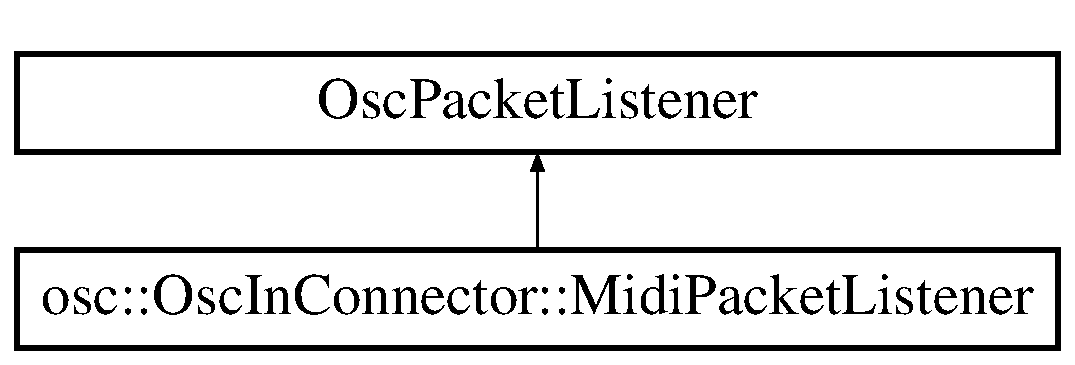
\includegraphics[height=2.000000cm]{classOscInConnector_1_1MidiPacketListener}
\end{center}
\end{figure}
\subsection*{Public Member Functions}
\begin{DoxyCompactItemize}
\item 
void {\bfseries set\+Osc\+In} (\hyperlink{classOscInConnector}{Osc\+In\+Connector} $\ast$o)\hypertarget{classOscInConnector_1_1MidiPacketListener_ab4e0346cad409b3871add20bc5c8c904}{}\label{classOscInConnector_1_1MidiPacketListener_ab4e0346cad409b3871add20bc5c8c904}

\item 
int {\bfseries get\+Port} ()\hypertarget{classOscInConnector_1_1MidiPacketListener_affd65358cd1ffcde113576b8023fa8d6}{}\label{classOscInConnector_1_1MidiPacketListener_affd65358cd1ffcde113576b8023fa8d6}

\end{DoxyCompactItemize}
\subsection*{Protected Member Functions}
\begin{DoxyCompactItemize}
\item 
void {\bfseries write\+Data} (std\+::string s, int a1, int a2, int a3, float f)\hypertarget{classOscInConnector_1_1MidiPacketListener_a6ad19bb71d7d360d432eecd4d2f8aa0f}{}\label{classOscInConnector_1_1MidiPacketListener_a6ad19bb71d7d360d432eecd4d2f8aa0f}

\item 
virtual void {\bfseries Process\+Message} (const osc\+::\+Received\+Message \&m, const Ip\+Endpoint\+Name \&remote\+Endpoint)\hypertarget{classOscInConnector_1_1MidiPacketListener_ad5b4e469c87859e8577d2bf77aaa66bd}{}\label{classOscInConnector_1_1MidiPacketListener_ad5b4e469c87859e8577d2bf77aaa66bd}

\end{DoxyCompactItemize}


The documentation for this class was generated from the following file\+:\begin{DoxyCompactItemize}
\item 
Osc\+In\+Connector.\+cpp\end{DoxyCompactItemize}

\hypertarget{classunit_1_1MultiplyGen}{}\section{unit\+:\+:Multiply\+Gen Class Reference}
\label{classunit_1_1MultiplyGen}\index{unit\+::\+Multiply\+Gen@{unit\+::\+Multiply\+Gen}}


{\ttfamily \#include $<$Multiply\+Gen.\+h$>$}

Inheritance diagram for unit\+:\+:Multiply\+Gen\+:\begin{figure}[H]
\begin{center}
\leavevmode
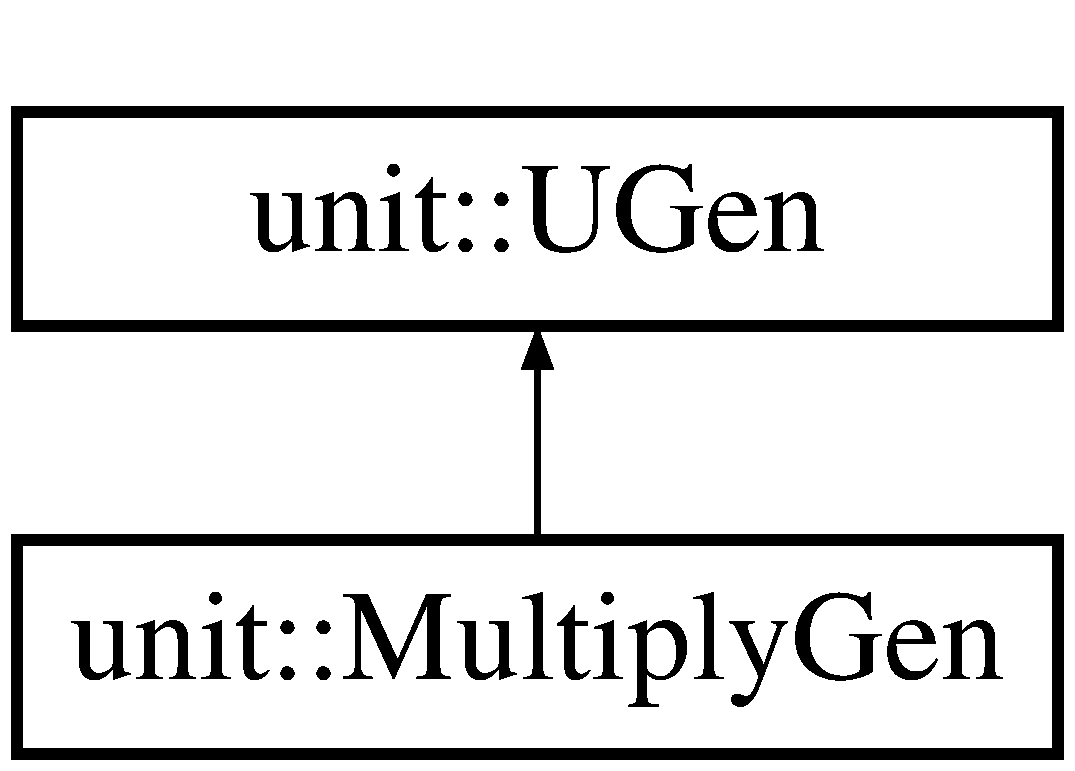
\includegraphics[height=2.000000cm]{classunit_1_1MultiplyGen}
\end{center}
\end{figure}
\subsection*{Public Member Functions}
\begin{DoxyCompactItemize}
\item 
{\bfseries Multiply\+Gen} (std\+::string name)\hypertarget{classunit_1_1MultiplyGen_a8c63aba9e9be634e03f900182b4a1d7a}{}\label{classunit_1_1MultiplyGen_a8c63aba9e9be634e03f900182b4a1d7a}

\item 
void {\bfseries control} (std\+::string port\+Name, float value)\hypertarget{classunit_1_1MultiplyGen_a399981309ef24f24c7044172e58c1e8a}{}\label{classunit_1_1MultiplyGen_a399981309ef24f24c7044172e58c1e8a}

\item 
float {\bfseries tick} ()\hypertarget{classunit_1_1MultiplyGen_abeeb8a84f91375454120639a9bb810fb}{}\label{classunit_1_1MultiplyGen_abeeb8a84f91375454120639a9bb810fb}

\end{DoxyCompactItemize}
\subsection*{Additional Inherited Members}


\subsection{Detailed Description}
\hyperlink{classunit_1_1MultiplyGen}{Multiply\+Gen} is a minimal mixing unit. It multiplies the {\bfseries in1} port with {\bfseries amnt1} port.


\begin{DoxyItemize}
\item {\bfseries tick()} is providing the product of {\bfseries in1} and {\bfseries amnt1}.
\end{DoxyItemize}

Control-\/\+Interface
\begin{DoxyItemize}
\item no control interface implemented
\end{DoxyItemize}

Fast access functions
\begin{DoxyItemize}
\item no further fast access functions implemented
\end{DoxyItemize}

\begin{DoxyAuthor}{Author}
jtm, email\+:  \href{mailto:milde@hs-fulda.de}{\tt milde@hs-\/fulda.\+de} 
\end{DoxyAuthor}
\begin{DoxySince}{Since}
04-\/2016 
\end{DoxySince}
\begin{DoxyVersion}{Version}
1.\+0 
\end{DoxyVersion}


The documentation for this class was generated from the following files\+:\begin{DoxyCompactItemize}
\item 
include/Multiply\+Gen.\+h\item 
unit/Multiply\+Gen.\+cpp\end{DoxyCompactItemize}

\hypertarget{classunit_1_1MultiplyTwoGen}{\section{unit\-:\-:Multiply\-Two\-Gen Class Reference}
\label{classunit_1_1MultiplyTwoGen}\index{unit\-::\-Multiply\-Two\-Gen@{unit\-::\-Multiply\-Two\-Gen}}
}


{\ttfamily \#include $<$Multiply\-Two\-Gen.\-h$>$}

Inheritance diagram for unit\-:\-:Multiply\-Two\-Gen\-:\begin{figure}[H]
\begin{center}
\leavevmode
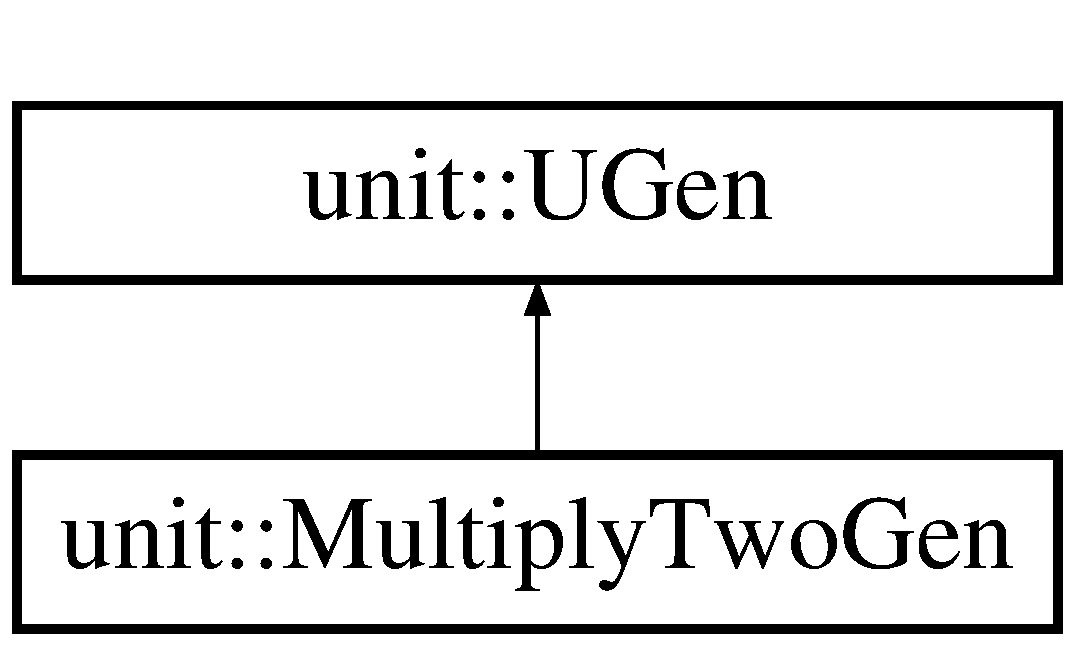
\includegraphics[height=2.000000cm]{classunit_1_1MultiplyTwoGen}
\end{center}
\end{figure}
\subsection*{Public Member Functions}
\begin{DoxyCompactItemize}
\item 
\hypertarget{classunit_1_1MultiplyTwoGen_a35e526170e8ac7a43fc19c2a78e14b44}{{\bfseries Multiply\-Two\-Gen} (std\-::string name)}\label{classunit_1_1MultiplyTwoGen_a35e526170e8ac7a43fc19c2a78e14b44}

\item 
\hypertarget{classunit_1_1MultiplyTwoGen_af8558651a63c73f27221e99ad03f3242}{void {\bfseries control} (std\-::string port\-Name, float value)}\label{classunit_1_1MultiplyTwoGen_af8558651a63c73f27221e99ad03f3242}

\item 
\hypertarget{classunit_1_1MultiplyTwoGen_a70a07ad9e0f67e6a50aadcdf902db8f3}{float {\bfseries tick} ()}\label{classunit_1_1MultiplyTwoGen_a70a07ad9e0f67e6a50aadcdf902db8f3}

\end{DoxyCompactItemize}
\subsection*{Additional Inherited Members}


\subsection{Detailed Description}
\hyperlink{classunit_1_1MultiplyTwoGen}{Multiply\-Two\-Gen} multiplies the two standard input ports in1 and in2.

\begin{DoxyAuthor}{Author}
jtm, email\-:  \href{mailto:milde@hs-fulda.de}{\tt milde@hs-\/fulda.\-de} 
\end{DoxyAuthor}
\begin{DoxySince}{Since}
04-\/2016 
\end{DoxySince}
\begin{DoxyVersion}{Version}
1.\-0 
\end{DoxyVersion}


The documentation for this class was generated from the following files\-:\begin{DoxyCompactItemize}
\item 
include/Multiply\-Two\-Gen.\-h\item 
unit/Multiply\-Two\-Gen.\-cpp\end{DoxyCompactItemize}

\hypertarget{classNeonlicht}{}\section{Neonlicht Class Reference}
\label{classNeonlicht}\index{Neonlicht@{Neonlicht}}
\subsection*{Public Member Functions}
\begin{DoxyCompactItemize}
\item 
void {\bfseries configure} ()\hypertarget{classNeonlicht_a32ec4c221148d01bbafd1637ced9b130}{}\label{classNeonlicht_a32ec4c221148d01bbafd1637ced9b130}

\item 
void {\bfseries start} ()\hypertarget{classNeonlicht_aae54e46be4d251ce4e062cd777994a69}{}\label{classNeonlicht_aae54e46be4d251ce4e062cd777994a69}

\item 
void {\bfseries stop} ()\hypertarget{classNeonlicht_a9d1f643b1a2394f9cd181149f7558c72}{}\label{classNeonlicht_a9d1f643b1a2394f9cd181149f7558c72}

\item 
long {\bfseries get\+Stream\+Latency} ()\hypertarget{classNeonlicht_a4354cc2fa6d7bd22e89d1314e375f54f}{}\label{classNeonlicht_a4354cc2fa6d7bd22e89d1314e375f54f}

\end{DoxyCompactItemize}
\subsection*{Static Public Member Functions}
\begin{DoxyCompactItemize}
\item 
static int {\bfseries tick} (void $\ast$output\+Buffer, void $\ast$input\+Buffer, unsigned int n\+Buffer\+Frames, double stream\+Time, Rt\+Audio\+Stream\+Status status, void $\ast$data\+Pointer)\hypertarget{classNeonlicht_a57c3e8d4154418c9efc4b48d45b732d6}{}\label{classNeonlicht_a57c3e8d4154418c9efc4b48d45b732d6}

\end{DoxyCompactItemize}
\subsection*{Static Public Attributes}
\begin{DoxyCompactItemize}
\item 
static \hyperlink{classCentralStore}{Central\+Store} {\bfseries CS}\hypertarget{classNeonlicht_a1ac3a31190125df3763a9f3d2f085d5e}{}\label{classNeonlicht_a1ac3a31190125df3763a9f3d2f085d5e}

\item 
static int {\bfseries C\+NT} = 0\hypertarget{classNeonlicht_ac86fbdabd4683feaac58b4aefbdf6695}{}\label{classNeonlicht_ac86fbdabd4683feaac58b4aefbdf6695}

\end{DoxyCompactItemize}


The documentation for this class was generated from the following files\+:\begin{DoxyCompactItemize}
\item 
include/Neonlicht.\+h\item 
Neonlicht.\+cpp\end{DoxyCompactItemize}

\hypertarget{classunit_1_1NoiseGen}{}\section{unit\+:\+:Noise\+Gen Class Reference}
\label{classunit_1_1NoiseGen}\index{unit\+::\+Noise\+Gen@{unit\+::\+Noise\+Gen}}


{\ttfamily \#include $<$Noise\+Gen.\+h$>$}

Inheritance diagram for unit\+:\+:Noise\+Gen\+:\begin{figure}[H]
\begin{center}
\leavevmode
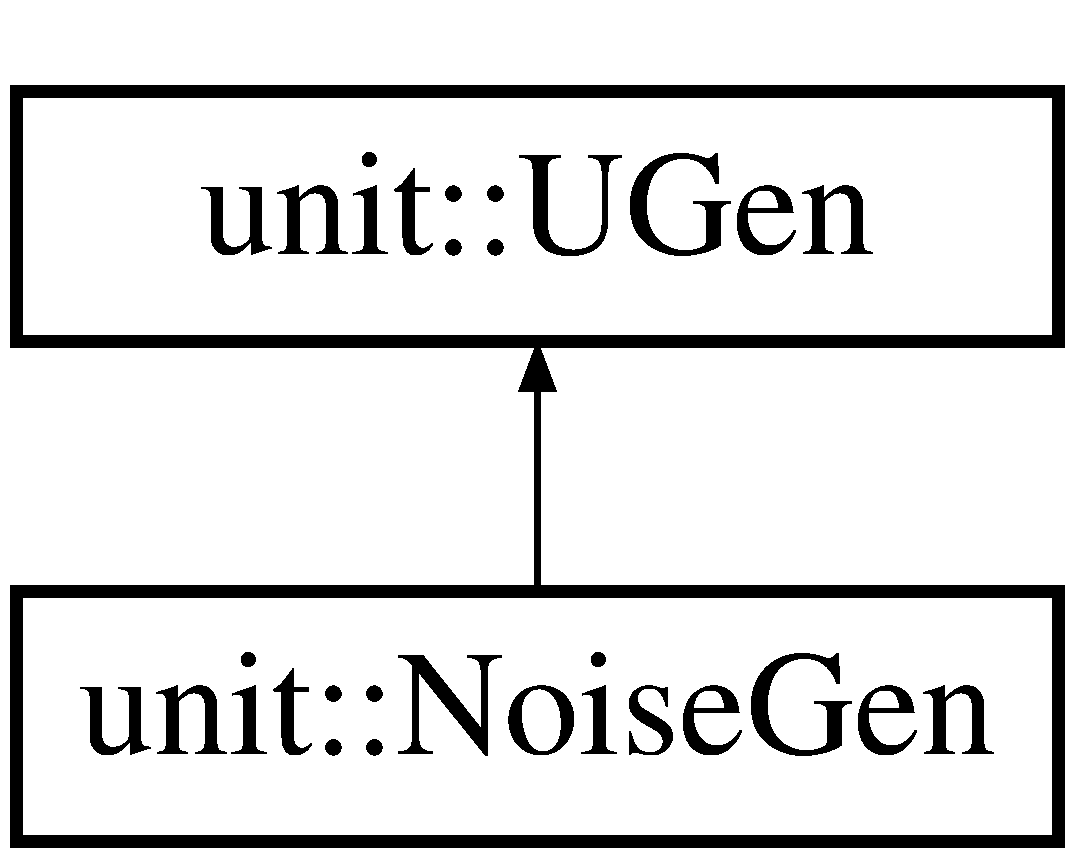
\includegraphics[height=3.000000cm]{classunit_1_1NoiseGen}
\end{center}
\end{figure}
\subsection*{Public Member Functions}
\begin{DoxyCompactItemize}
\item 
{\bfseries Noise\+Gen} (std\+::string name)\hypertarget{classunit_1_1NoiseGen_aa49d8817fff2757abc19f0dffea0c7fe}{}\label{classunit_1_1NoiseGen_aa49d8817fff2757abc19f0dffea0c7fe}

\item 
void {\bfseries control} (std\+::string port\+Name, float value)\hypertarget{classunit_1_1NoiseGen_a73628ae13d893658b88bc30eb43437ba}{}\label{classunit_1_1NoiseGen_a73628ae13d893658b88bc30eb43437ba}

\item 
float {\bfseries tick} ()\hypertarget{classunit_1_1NoiseGen_addaecf96df1cf9f1ba4875fb849949df}{}\label{classunit_1_1NoiseGen_addaecf96df1cf9f1ba4875fb849949df}

\end{DoxyCompactItemize}
\subsection*{Public Attributes}
\begin{DoxyCompactItemize}
\item 
long {\bfseries count} = 0\hypertarget{classunit_1_1NoiseGen_a9509da6dba8e294d3e5bc26d2eb6d39f}{}\label{classunit_1_1NoiseGen_a9509da6dba8e294d3e5bc26d2eb6d39f}

\end{DoxyCompactItemize}
\subsection*{Additional Inherited Members}


\subsection{Detailed Description}
\hyperlink{classunit_1_1NoiseGen}{Noise\+Gen} generates white noise.


\begin{DoxyItemize}
\item {\bfseries tick()} is providing a random value in the range of \mbox{[}-\/1,1\mbox{]}.
\end{DoxyItemize}

Control-\/\+Interface
\begin{DoxyItemize}
\item no control interface implemented
\end{DoxyItemize}

Fast access functions
\begin{DoxyItemize}
\item no further fast access functions implemented
\end{DoxyItemize}

\begin{DoxyAuthor}{Author}
jtm, email\+:  \href{mailto:milde@hs-fulda.de}{\tt milde@hs-\/fulda.\+de} 
\end{DoxyAuthor}
\begin{DoxySince}{Since}
04-\/2016 
\end{DoxySince}
\begin{DoxyVersion}{Version}
1.\+0 
\end{DoxyVersion}


The documentation for this class was generated from the following files\+:\begin{DoxyCompactItemize}
\item 
include/Noise\+Gen.\+h\item 
unit/Noise\+Gen.\+cpp\end{DoxyCompactItemize}

\hypertarget{classNoiseUnit}{}\section{Noise\+Unit Class Reference}
\label{classNoiseUnit}\index{Noise\+Unit@{Noise\+Unit}}
Inheritance diagram for Noise\+Unit\+:\begin{figure}[H]
\begin{center}
\leavevmode
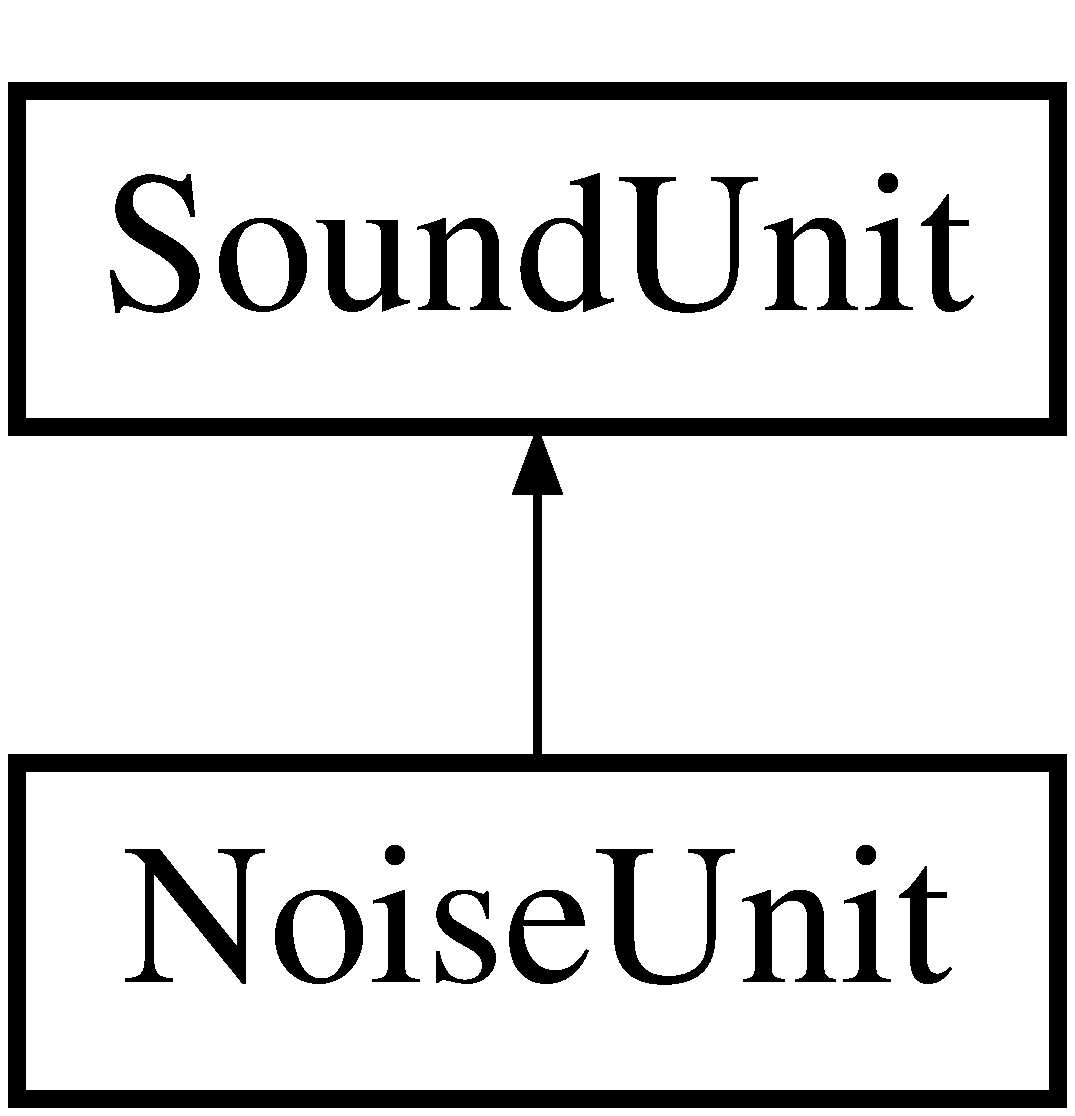
\includegraphics[height=2.000000cm]{classNoiseUnit}
\end{center}
\end{figure}
\subsection*{Public Member Functions}
\begin{DoxyCompactItemize}
\item 
void {\bfseries setup} ()\hypertarget{classNoiseUnit_a81666e8bdea833fad6a4451a765c6b83}{}\label{classNoiseUnit_a81666e8bdea833fad6a4451a765c6b83}

\item 
void {\bfseries control} (std\+::string port\+Name, float value)\hypertarget{classNoiseUnit_a7014ea85fb499bbe69fcf7ce96be8d32}{}\label{classNoiseUnit_a7014ea85fb499bbe69fcf7ce96be8d32}

\item 
float {\bfseries tick} ()\hypertarget{classNoiseUnit_af48a9a915f7f593105e8fe2d2ddb745a}{}\label{classNoiseUnit_af48a9a915f7f593105e8fe2d2ddb745a}

\end{DoxyCompactItemize}
\subsection*{Additional Inherited Members}


The documentation for this class was generated from the following files\+:\begin{DoxyCompactItemize}
\item 
unit/Noise\+Unit.\+h\item 
unit/Noise\+Unit.\+cpp\end{DoxyCompactItemize}

\hypertarget{classunit_1_1NumberGen}{}\section{unit\+:\+:Number\+Gen Class Reference}
\label{classunit_1_1NumberGen}\index{unit\+::\+Number\+Gen@{unit\+::\+Number\+Gen}}


{\ttfamily \#include $<$Number\+Gen.\+h$>$}

Inheritance diagram for unit\+:\+:Number\+Gen\+:\begin{figure}[H]
\begin{center}
\leavevmode
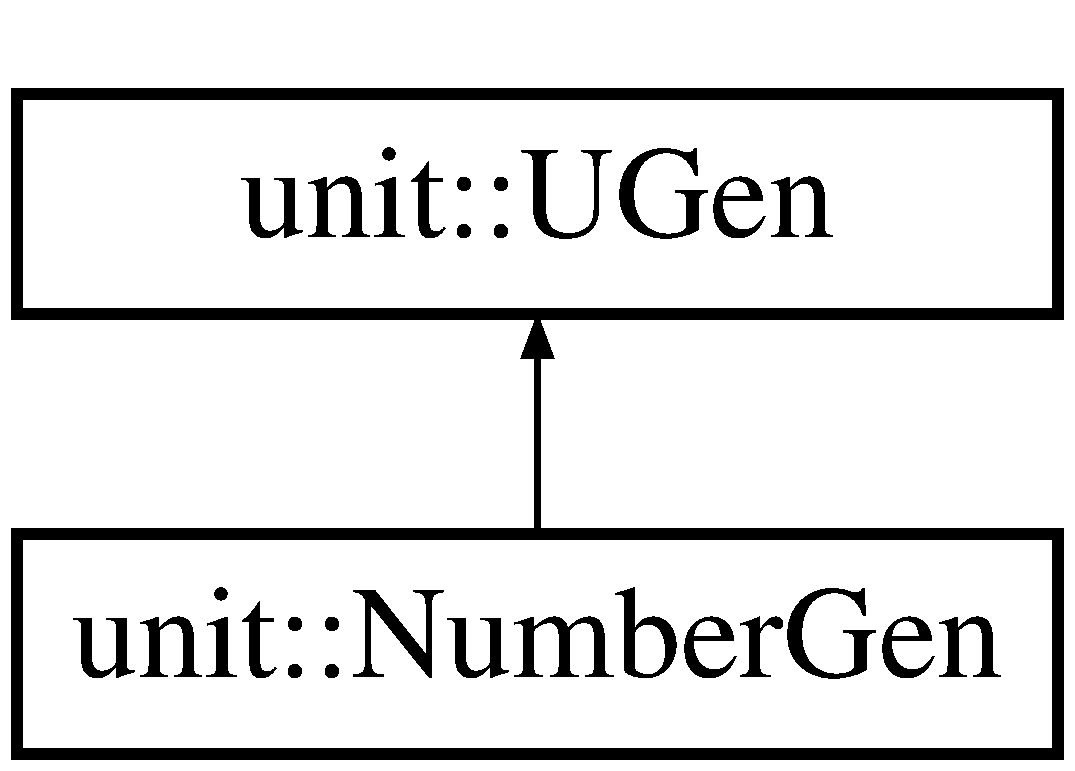
\includegraphics[height=2.000000cm]{classunit_1_1NumberGen}
\end{center}
\end{figure}
\subsection*{Public Member Functions}
\begin{DoxyCompactItemize}
\item 
{\bfseries Number\+Gen} (std\+::string name)\hypertarget{classunit_1_1NumberGen_a6e93812c4805a43f19f8fb11680e32a4}{}\label{classunit_1_1NumberGen_a6e93812c4805a43f19f8fb11680e32a4}

\item 
void {\bfseries control} (std\+::string port\+Name, float value)\hypertarget{classunit_1_1NumberGen_a9daaaf8a12389873494bb1ad2f877c8c}{}\label{classunit_1_1NumberGen_a9daaaf8a12389873494bb1ad2f877c8c}

\item 
float {\bfseries tick} ()\hypertarget{classunit_1_1NumberGen_a38cef7d64a12e40bf2ae14f29def41ca}{}\label{classunit_1_1NumberGen_a38cef7d64a12e40bf2ae14f29def41ca}

\item 
void {\bfseries set\+Value} (float value)\hypertarget{classunit_1_1NumberGen_ad5c107c90a5bc6cf7bbc39562db9d9e3}{}\label{classunit_1_1NumberGen_ad5c107c90a5bc6cf7bbc39562db9d9e3}

\end{DoxyCompactItemize}
\subsection*{Additional Inherited Members}


\subsection{Detailed Description}
\hyperlink{classunit_1_1NumberGen}{Number\+Gen} stores a value.


\begin{DoxyItemize}
\item {\bfseries tick()} is providing the stored value.
\end{DoxyItemize}

Control-\/\+Interface -\/$\ast$$\ast$control(\char`\"{}non empty string\char`\"{}, value)$\ast$$\ast$\+: stores the value in amnt1. The port\+Name has to be a non empty string, otherwise the value will not be stored.

Fast access functions
\begin{DoxyItemize}
\item {\bfseries set\+Value(float value)}\+: stores the value in amnt1 (and in out1).
\end{DoxyItemize}

\begin{DoxyAuthor}{Author}
jtm, email\+:  \href{mailto:milde@hs-fulda.de}{\tt milde@hs-\/fulda.\+de} 
\end{DoxyAuthor}
\begin{DoxySince}{Since}
04-\/2016 
\end{DoxySince}
\begin{DoxyVersion}{Version}
1.\+0 
\end{DoxyVersion}


The documentation for this class was generated from the following files\+:\begin{DoxyCompactItemize}
\item 
include/Number\+Gen.\+h\item 
unit/Number\+Gen.\+cpp\end{DoxyCompactItemize}

\hypertarget{classunit_1_1OnePoleLPFGen}{}\section{unit\+:\+:One\+Pole\+L\+P\+F\+Gen Class Reference}
\label{classunit_1_1OnePoleLPFGen}\index{unit\+::\+One\+Pole\+L\+P\+F\+Gen@{unit\+::\+One\+Pole\+L\+P\+F\+Gen}}
Inheritance diagram for unit\+:\+:One\+Pole\+L\+P\+F\+Gen\+:\begin{figure}[H]
\begin{center}
\leavevmode
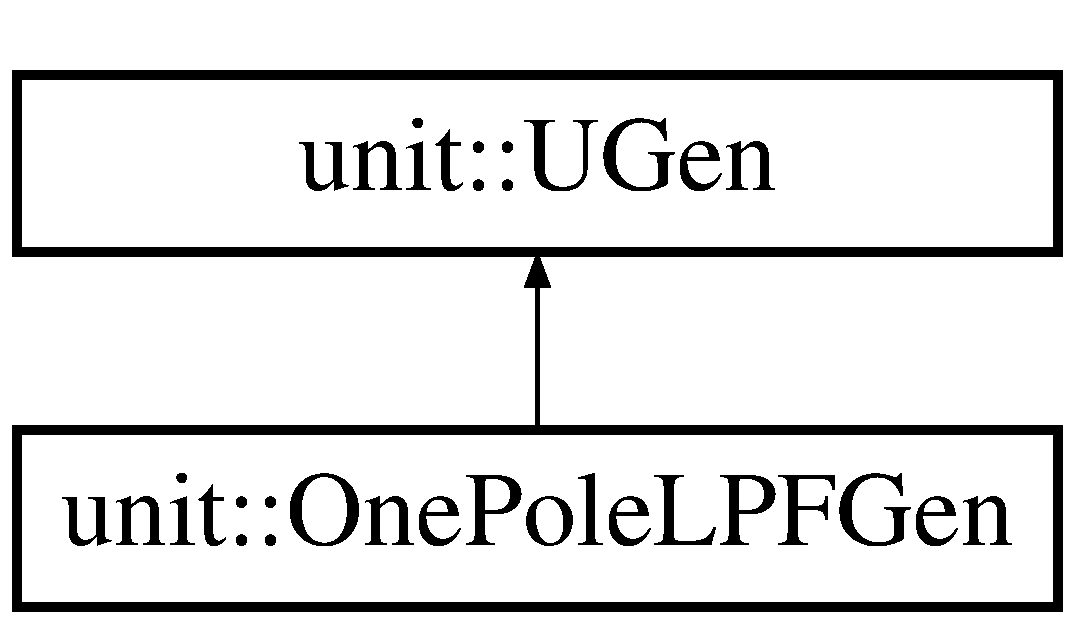
\includegraphics[height=2.000000cm]{classunit_1_1OnePoleLPFGen}
\end{center}
\end{figure}
\subsection*{Public Member Functions}
\begin{DoxyCompactItemize}
\item 
{\bfseries One\+Pole\+L\+P\+F\+Gen} (std\+::string name)\hypertarget{classunit_1_1OnePoleLPFGen_aea39a9562852ac47fdd576fd8b583b9f}{}\label{classunit_1_1OnePoleLPFGen_aea39a9562852ac47fdd576fd8b583b9f}

\item 
void {\bfseries control} (std\+::string port\+Name, float value)\hypertarget{classunit_1_1OnePoleLPFGen_a8f2df9b7406edadf7dc34e7e65b2b67c}{}\label{classunit_1_1OnePoleLPFGen_a8f2df9b7406edadf7dc34e7e65b2b67c}

\item 
float {\bfseries tick} ()\hypertarget{classunit_1_1OnePoleLPFGen_a5e5288841ff8112113f2d6ec1f03f375}{}\label{classunit_1_1OnePoleLPFGen_a5e5288841ff8112113f2d6ec1f03f375}

\end{DoxyCompactItemize}
\subsection*{Additional Inherited Members}


The documentation for this class was generated from the following files\+:\begin{DoxyCompactItemize}
\item 
unit/One\+Pole\+L\+P\+F\+Gen.\+h\item 
unit/One\+Pole\+L\+P\+F\+Gen.\+cpp\end{DoxyCompactItemize}

\hypertarget{classOscActivator}{}\section{Osc\+Activator Class Reference}
\label{classOscActivator}\index{Osc\+Activator@{Osc\+Activator}}
Inheritance diagram for Osc\+Activator\+:\begin{figure}[H]
\begin{center}
\leavevmode
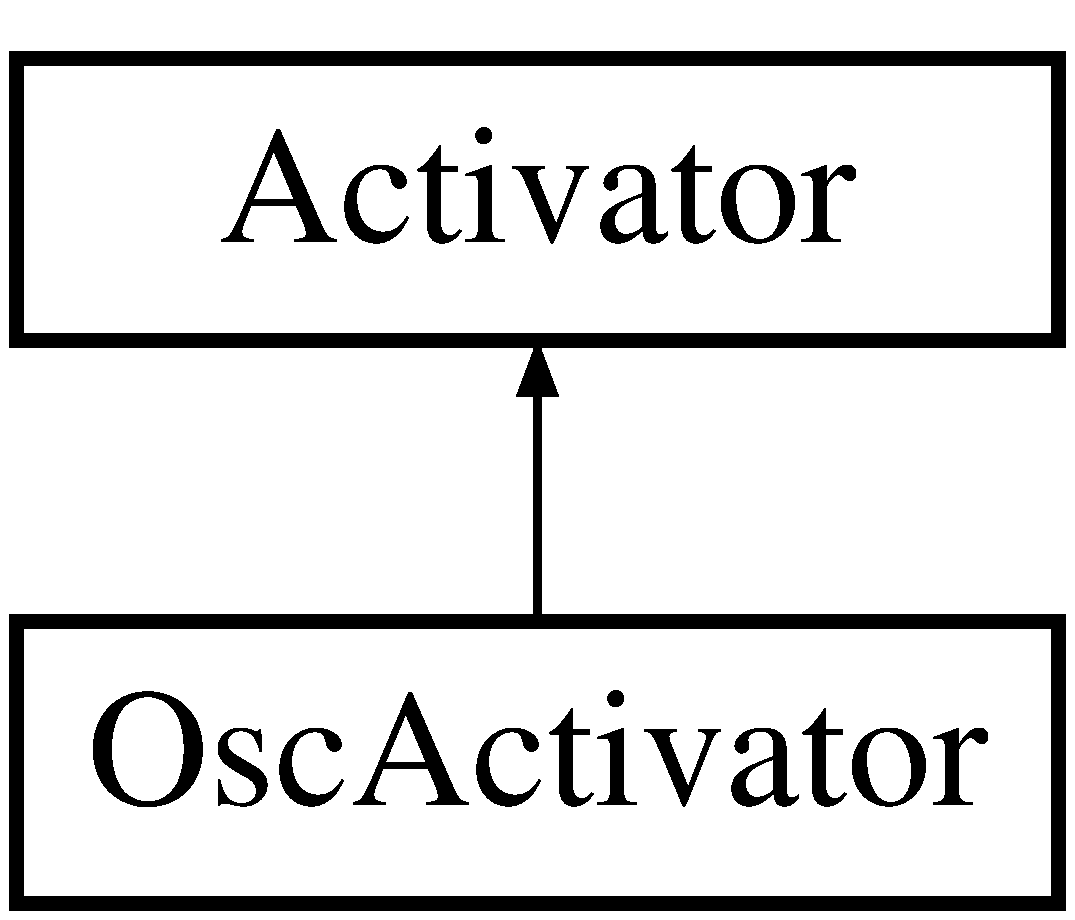
\includegraphics[height=2.000000cm]{classOscActivator}
\end{center}
\end{figure}
\subsection*{Public Member Functions}
\begin{DoxyCompactItemize}
\item 
void {\bfseries callback} (float value)\hypertarget{classOscActivator_ad5852376e949408b2fc13c8adf60c032}{}\label{classOscActivator_ad5852376e949408b2fc13c8adf60c032}

\end{DoxyCompactItemize}


The documentation for this class was generated from the following files\+:\begin{DoxyCompactItemize}
\item 
sequencer/Osc\+Activator.\+h\item 
sequencer/Osc\+Activator.\+cpp\end{DoxyCompactItemize}

\hypertarget{classOscInConnector}{}\section{Osc\+In\+Connector Class Reference}
\label{classOscInConnector}\index{Osc\+In\+Connector@{Osc\+In\+Connector}}
\subsection*{Classes}
\begin{DoxyCompactItemize}
\item 
class \hyperlink{classOscInConnector_1_1MidiPacketListener}{Midi\+Packet\+Listener}
\end{DoxyCompactItemize}
\subsection*{Public Member Functions}
\begin{DoxyCompactItemize}
\item 
{\bfseries Osc\+In\+Connector} (int prt)\hypertarget{classOscInConnector_acb8cca9cec941690ed0dcee6611c4553}{}\label{classOscInConnector_acb8cca9cec941690ed0dcee6611c4553}

\item 
bool {\bfseries is\+Fresh} ()\hypertarget{classOscInConnector_a6603048c9ba0e9356a8dd0f5ffc1055f}{}\label{classOscInConnector_a6603048c9ba0e9356a8dd0f5ffc1055f}

\item 
\hyperlink{classMessageData}{Message\+Data} $\ast$ {\bfseries get\+Data} ()\hypertarget{classOscInConnector_aa7130d46061b498d0f8648c0bd9c4146}{}\label{classOscInConnector_aa7130d46061b498d0f8648c0bd9c4146}

\item 
std\+::thread \hyperlink{classOscInConnector_af546d19cf2adc1ed7c701a4804586cb9}{start\+Thread} ()
\end{DoxyCompactItemize}
\subsection*{Public Attributes}
\begin{DoxyCompactItemize}
\item 
\hyperlink{classMessageData}{Message\+Data} $\ast$ {\bfseries MD} = new \hyperlink{classMessageData}{Message\+Data}(\char`\"{}xxx\char`\"{},1,2,3,3.\+14f)\hypertarget{classOscInConnector_a5ff52e9ac740d92aec0eb9f1eee00ddf}{}\label{classOscInConnector_a5ff52e9ac740d92aec0eb9f1eee00ddf}

\item 
bool {\bfseries talk} = true\hypertarget{classOscInConnector_a0472faba62d4db290aeb71326b31d5cc}{}\label{classOscInConnector_a0472faba62d4db290aeb71326b31d5cc}

\end{DoxyCompactItemize}


\subsection{Member Function Documentation}
\index{Osc\+In\+Connector@{Osc\+In\+Connector}!start\+Thread@{start\+Thread}}
\index{start\+Thread@{start\+Thread}!Osc\+In\+Connector@{Osc\+In\+Connector}}
\subsubsection[{\texorpdfstring{start\+Thread()}{startThread()}}]{\setlength{\rightskip}{0pt plus 5cm}std\+::thread Osc\+In\+Connector\+::start\+Thread (
\begin{DoxyParamCaption}
{}
\end{DoxyParamCaption}
)}\hypertarget{classOscInConnector_af546d19cf2adc1ed7c701a4804586cb9}{}\label{classOscInConnector_af546d19cf2adc1ed7c701a4804586cb9}
Scheint zu funktionieren, keine Ahnung warum \+:) 

The documentation for this class was generated from the following files\+:\begin{DoxyCompactItemize}
\item 
osc/Osc\+In\+Connector.\+h\item 
osc/Osc\+In\+Connector.\+cpp\end{DoxyCompactItemize}

\hypertarget{classOscOutConnector}{}\section{Osc\+Out\+Connector Class Reference}
\label{classOscOutConnector}\index{Osc\+Out\+Connector@{Osc\+Out\+Connector}}
\subsection*{Public Member Functions}
\begin{DoxyCompactItemize}
\item 
{\bfseries Osc\+Out\+Connector} (std\+::string h, int p)\hypertarget{classOscOutConnector_a7dde00203135c4a673e56f02dec774b4}{}\label{classOscOutConnector_a7dde00203135c4a673e56f02dec774b4}

\item 
void {\bfseries send\+Message} (std\+::string s, int a1, int a2, int a3, float f1)\hypertarget{classOscOutConnector_a8b3bcadf0295998b42753161ae9d17ee}{}\label{classOscOutConnector_a8b3bcadf0295998b42753161ae9d17ee}

\end{DoxyCompactItemize}


The documentation for this class was generated from the following files\+:\begin{DoxyCompactItemize}
\item 
Osc\+Out\+Connector.\+h\item 
Osc\+Out\+Connector.\+cpp\end{DoxyCompactItemize}

\hypertarget{classOscWrapper}{\section{Osc\-Wrapper Class Reference}
\label{classOscWrapper}\index{Osc\-Wrapper@{Osc\-Wrapper}}
}


The documentation for this class was generated from the following files\-:\begin{DoxyCompactItemize}
\item 
include/Osc\-Wrapper.\-h\item 
store/Osc\-Wrapper.\-cpp\end{DoxyCompactItemize}

\hypertarget{classPatch}{}\section{Patch Class Reference}
\label{classPatch}\index{Patch@{Patch}}
\subsection*{Public Member Functions}
\begin{DoxyCompactItemize}
\item 
{\bfseries Patch} (std\+::string from, int pt\+From, std\+::string to, int p\+To)\hypertarget{classPatch_a5ff9de0f83c44aa11aae837870aa55f0}{}\label{classPatch_a5ff9de0f83c44aa11aae837870aa55f0}

\item 
std\+::string {\bfseries get\+From} ()\hypertarget{classPatch_a97b08ef9e08c5ef8b5d71692a7242796}{}\label{classPatch_a97b08ef9e08c5ef8b5d71692a7242796}

\item 
int {\bfseries get\+From\+Port} ()\hypertarget{classPatch_a365988c401459bfd0f0b5b21f041bfe1}{}\label{classPatch_a365988c401459bfd0f0b5b21f041bfe1}

\item 
std\+::string {\bfseries get\+To} ()\hypertarget{classPatch_ade1fb3107faa8224f29c4a8387821fee}{}\label{classPatch_ade1fb3107faa8224f29c4a8387821fee}

\item 
int {\bfseries get\+Form\+Port} ()\hypertarget{classPatch_a19e489d67f86b80ac5f0ef774a3b87c8}{}\label{classPatch_a19e489d67f86b80ac5f0ef774a3b87c8}

\end{DoxyCompactItemize}


The documentation for this class was generated from the following files\+:\begin{DoxyCompactItemize}
\item 
unit/Patch.\+h\item 
unit/Patch.\+cpp\end{DoxyCompactItemize}

\hypertarget{classunit_1_1PhasorGen}{\section{unit\-:\-:Phasor\-Gen Class Reference}
\label{classunit_1_1PhasorGen}\index{unit\-::\-Phasor\-Gen@{unit\-::\-Phasor\-Gen}}
}


{\ttfamily \#include $<$Phasor\-Gen.\-h$>$}

Inheritance diagram for unit\-:\-:Phasor\-Gen\-:\begin{figure}[H]
\begin{center}
\leavevmode
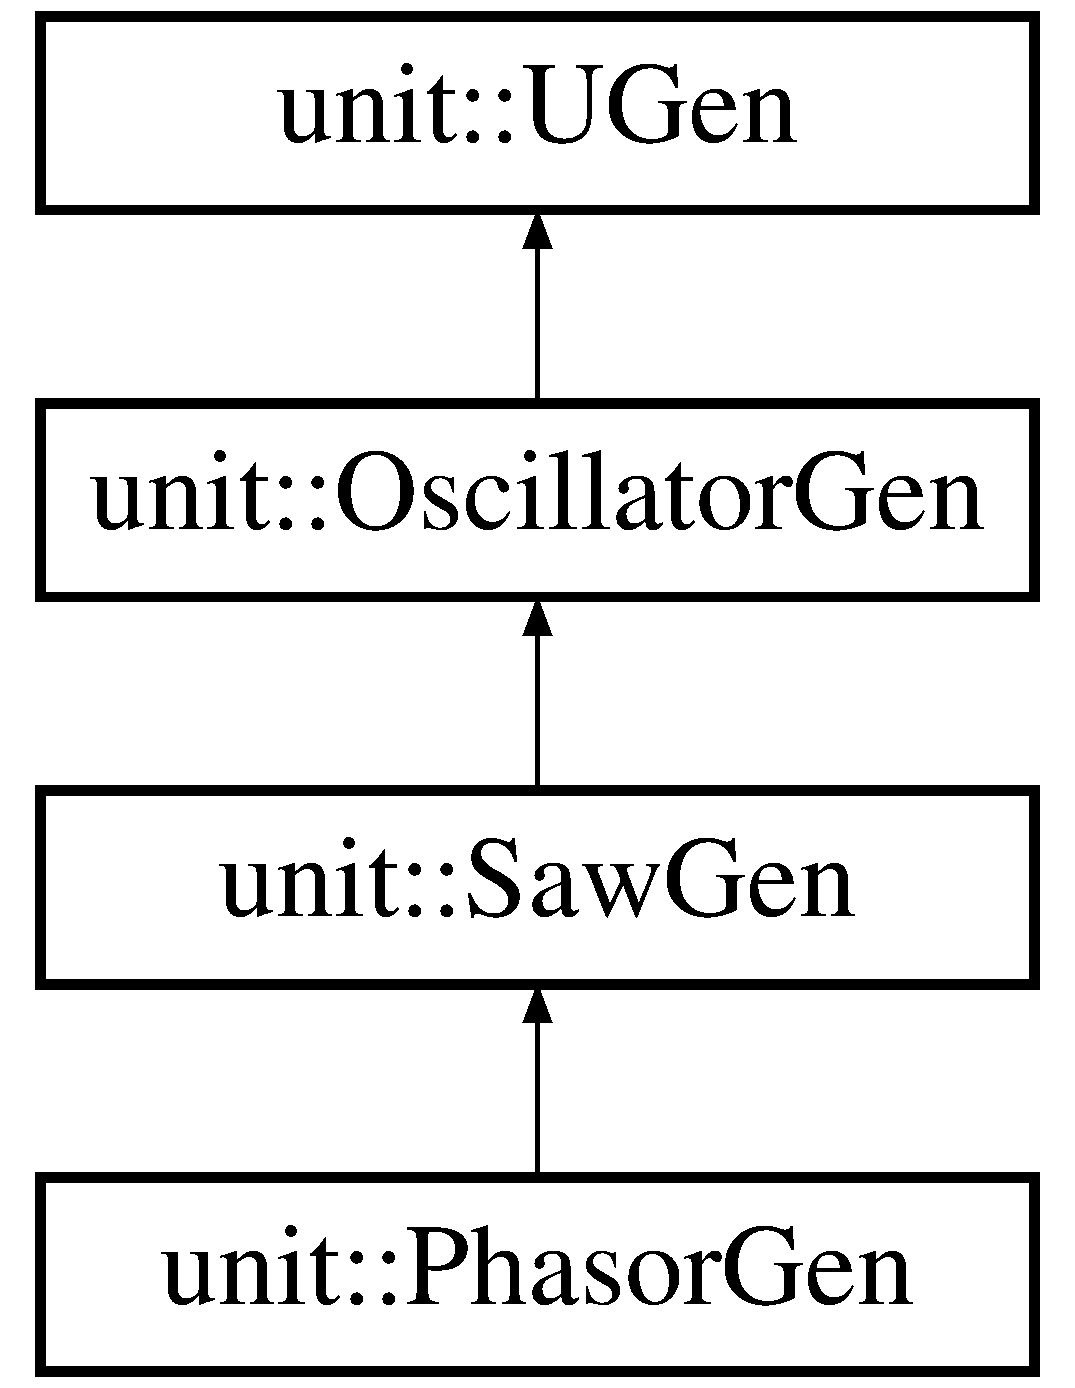
\includegraphics[height=4.000000cm]{classunit_1_1PhasorGen}
\end{center}
\end{figure}
\subsection*{Public Member Functions}
\begin{DoxyCompactItemize}
\item 
\hypertarget{classunit_1_1PhasorGen_a726fab6730e45d7fbf242f4613837e28}{{\bfseries Phasor\-Gen} (std\-::string name)}\label{classunit_1_1PhasorGen_a726fab6730e45d7fbf242f4613837e28}

\item 
\hypertarget{classunit_1_1PhasorGen_a056953090628af9868e4778d15daf79a}{float {\bfseries tick} ()}\label{classunit_1_1PhasorGen_a056953090628af9868e4778d15daf79a}

\end{DoxyCompactItemize}
\subsection*{Additional Inherited Members}


\subsection{Detailed Description}
\hyperlink{classunit_1_1PhasorGen}{Phasor\-Gen} generates a standard ramp \mbox{[}0,1\mbox{]}.

\begin{DoxyAuthor}{Author}
jtm, email\-:  \href{mailto:milde@hs-fulda.de}{\tt milde@hs-\/fulda.\-de} 
\end{DoxyAuthor}
\begin{DoxySince}{Since}
04-\/2016 
\end{DoxySince}
\begin{DoxyVersion}{Version}
1.\-0 
\end{DoxyVersion}


The documentation for this class was generated from the following files\-:\begin{DoxyCompactItemize}
\item 
src/include/Phasor\-Gen.\-h\item 
src/unit/Phasor\-Gen.\-cpp\end{DoxyCompactItemize}

\hypertarget{classPort}{\section{Port Class Reference}
\label{classPort}\index{Port@{Port}}
}
\subsection*{Public Member Functions}
\begin{DoxyCompactItemize}
\item 
\hypertarget{classPort_aadff8efe873e31b3362dda2b4a28c8c9}{{\bfseries Port} (std\-::string name, Port\-Type t)}\label{classPort_aadff8efe873e31b3362dda2b4a28c8c9}

\item 
\hypertarget{classPort_ad2c3baf0b291aee3b5b65178231754a6}{std\-::string {\bfseries get\-Name} ()}\label{classPort_ad2c3baf0b291aee3b5b65178231754a6}

\item 
\hypertarget{classPort_a31744528a5ade68a59ce094f3797bc1e}{std\-::string {\bfseries get\-I\-D} ()}\label{classPort_a31744528a5ade68a59ce094f3797bc1e}

\item 
\hypertarget{classPort_a5859f5d788d56c0103f4274b6d62b725}{Port\-Type {\bfseries get\-Type} ()}\label{classPort_a5859f5d788d56c0103f4274b6d62b725}

\item 
\hypertarget{classPort_a101b9cfba62777fb61c35a642b63f25a}{float {\bfseries get\-Value} ()}\label{classPort_a101b9cfba62777fb61c35a642b63f25a}

\item 
\hypertarget{classPort_afc93a217ba756e559c157b66745823a7}{void {\bfseries set\-Value} (float v)}\label{classPort_afc93a217ba756e559c157b66745823a7}

\end{DoxyCompactItemize}


The documentation for this class was generated from the following files\-:\begin{DoxyCompactItemize}
\item 
src/include/Port.\-h\item 
src/unit/Port.\-cpp\end{DoxyCompactItemize}

\hypertarget{classPulse}{\section{Pulse Class Reference}
\label{classPulse}\index{Pulse@{Pulse}}
}


{\ttfamily \#include $<$Pulse.\-h$>$}

\subsection*{Public Member Functions}
\begin{DoxyCompactItemize}
\item 
\hypertarget{classPulse_a9835b637db766732dd508c94fc30c501}{{\bfseries Pulse} (float bpm)}\label{classPulse_a9835b637db766732dd508c94fc30c501}

\item 
\hypertarget{classPulse_a164d81d4e1e798a5eec15b0b030b4047}{void {\bfseries start} ()}\label{classPulse_a164d81d4e1e798a5eec15b0b030b4047}

\item 
\hypertarget{classPulse_a7c8121986bec5319bb097216fe5e93d0}{void {\bfseries stop} ()}\label{classPulse_a7c8121986bec5319bb097216fe5e93d0}

\item 
\hypertarget{classPulse_a8283f4ab252e0c38b1e19a4dec522f23}{void {\bfseries set\-Activator} (\hyperlink{classActivator}{Activator} $\ast$a)}\label{classPulse_a8283f4ab252e0c38b1e19a4dec522f23}

\item 
\hypertarget{classPulse_afc87b2e4120c47942cf03fc82aaf8002}{void {\bfseries set\-Speed} (float bpm)}\label{classPulse_afc87b2e4120c47942cf03fc82aaf8002}

\end{DoxyCompactItemize}


\subsection{Detailed Description}
\hyperlink{classPulse}{Pulse} generates a beat and sends the pulses to an \hyperlink{classActivator}{Activator}. The pulse is quantized to a zweiundreissigstel (thirty second note/demisemiquaver).

\begin{DoxyAuthor}{Author}
jtm, email\-:  \href{mailto:milde@hs-fulda.de}{\tt milde@hs-\/fulda.\-de} 
\end{DoxyAuthor}
\begin{DoxySince}{Since}
04-\/2016 
\end{DoxySince}
\begin{DoxyVersion}{Version}
1.\-0 
\end{DoxyVersion}


The documentation for this class was generated from the following files\-:\begin{DoxyCompactItemize}
\item 
include/Pulse.\-h\item 
sequencer/Pulse.\-cpp\end{DoxyCompactItemize}

\hypertarget{classunit_1_1SawGen}{\section{unit\-:\-:Saw\-Gen Class Reference}
\label{classunit_1_1SawGen}\index{unit\-::\-Saw\-Gen@{unit\-::\-Saw\-Gen}}
}


{\ttfamily \#include $<$Saw\-Gen.\-h$>$}

Inheritance diagram for unit\-:\-:Saw\-Gen\-:\begin{figure}[H]
\begin{center}
\leavevmode
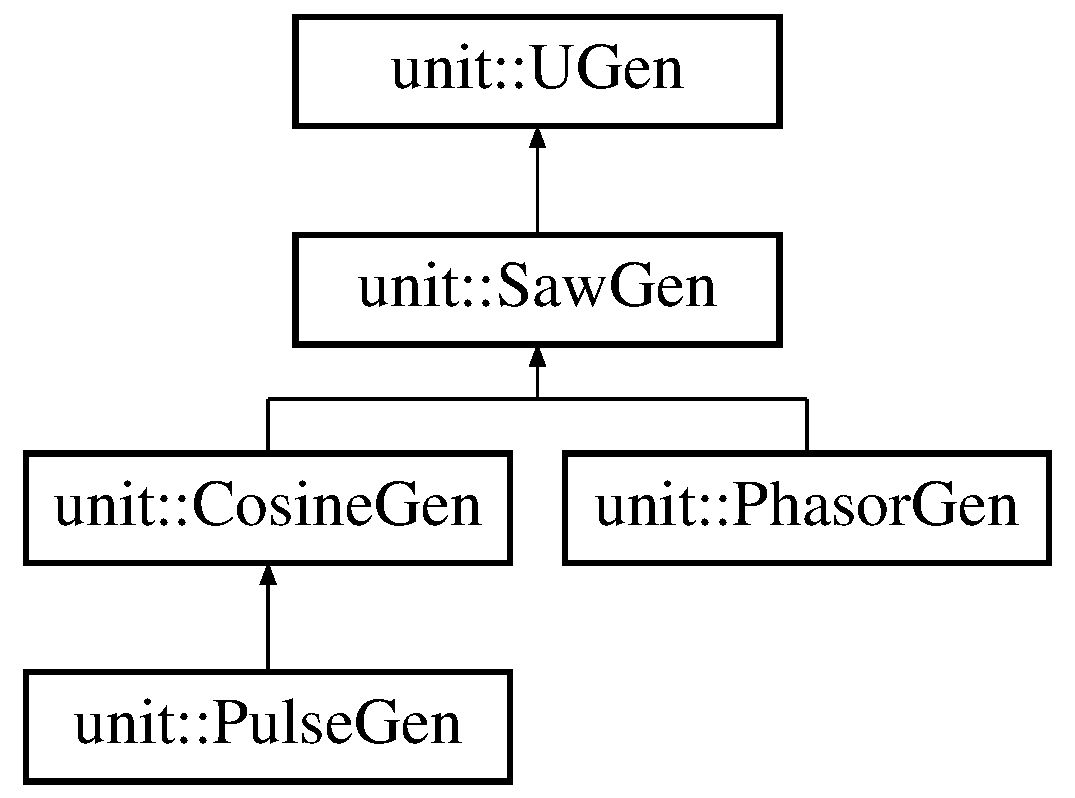
\includegraphics[height=6.000000cm]{classunit_1_1SawGen}
\end{center}
\end{figure}
\subsection*{Public Member Functions}
\begin{DoxyCompactItemize}
\item 
\hypertarget{classunit_1_1SawGen_a24c35afc1bdb237a8a5d1eb3888ce0bc}{{\bfseries Saw\-Gen} (std\-::string name)}\label{classunit_1_1SawGen_a24c35afc1bdb237a8a5d1eb3888ce0bc}

\item 
\hypertarget{classunit_1_1SawGen_a515f6eb82a1a97ee434144b8c58133b8}{void {\bfseries control} (std\-::string port\-Name, float value)}\label{classunit_1_1SawGen_a515f6eb82a1a97ee434144b8c58133b8}

\item 
\hypertarget{classunit_1_1SawGen_a18c6704aec8f20a5605ff72d674c7516}{float {\bfseries tick} ()}\label{classunit_1_1SawGen_a18c6704aec8f20a5605ff72d674c7516}

\item 
\hypertarget{classunit_1_1SawGen_a1a77058c93e7f7b3fe4b355953674678}{void {\bfseries set\-Frequency} (float value)}\label{classunit_1_1SawGen_a1a77058c93e7f7b3fe4b355953674678}

\item 
\hypertarget{classunit_1_1SawGen_a0f08973bebb28aa1a059ccce09e5ebdf}{float {\bfseries get\-Frequency} ()}\label{classunit_1_1SawGen_a0f08973bebb28aa1a059ccce09e5ebdf}

\end{DoxyCompactItemize}
\subsection*{Additional Inherited Members}


\subsection{Detailed Description}
\hyperlink{classunit_1_1SawGen}{Saw\-Gen} generates a saw wave based on a simple linear interpolation.

The implementation is not very effective and needs to be redone. It also contains an implementation error. It should use a wave table.

\begin{DoxyAuthor}{Author}
jtm, email\-:  \href{mailto:milde@hs-fulda.de}{\tt milde@hs-\/fulda.\-de} 
\end{DoxyAuthor}
\begin{DoxySince}{Since}
04-\/2016 
\end{DoxySince}
\begin{DoxyVersion}{Version}
1.\-0 
\end{DoxyVersion}


The documentation for this class was generated from the following files\-:\begin{DoxyCompactItemize}
\item 
include/Saw\-Gen.\-h\item 
unit/Saw\-Gen.\-cpp\end{DoxyCompactItemize}

\hypertarget{classSoundUnit}{}\section{Sound\+Unit Class Reference}
\label{classSoundUnit}\index{Sound\+Unit@{Sound\+Unit}}
Inheritance diagram for Sound\+Unit\+:\begin{figure}[H]
\begin{center}
\leavevmode
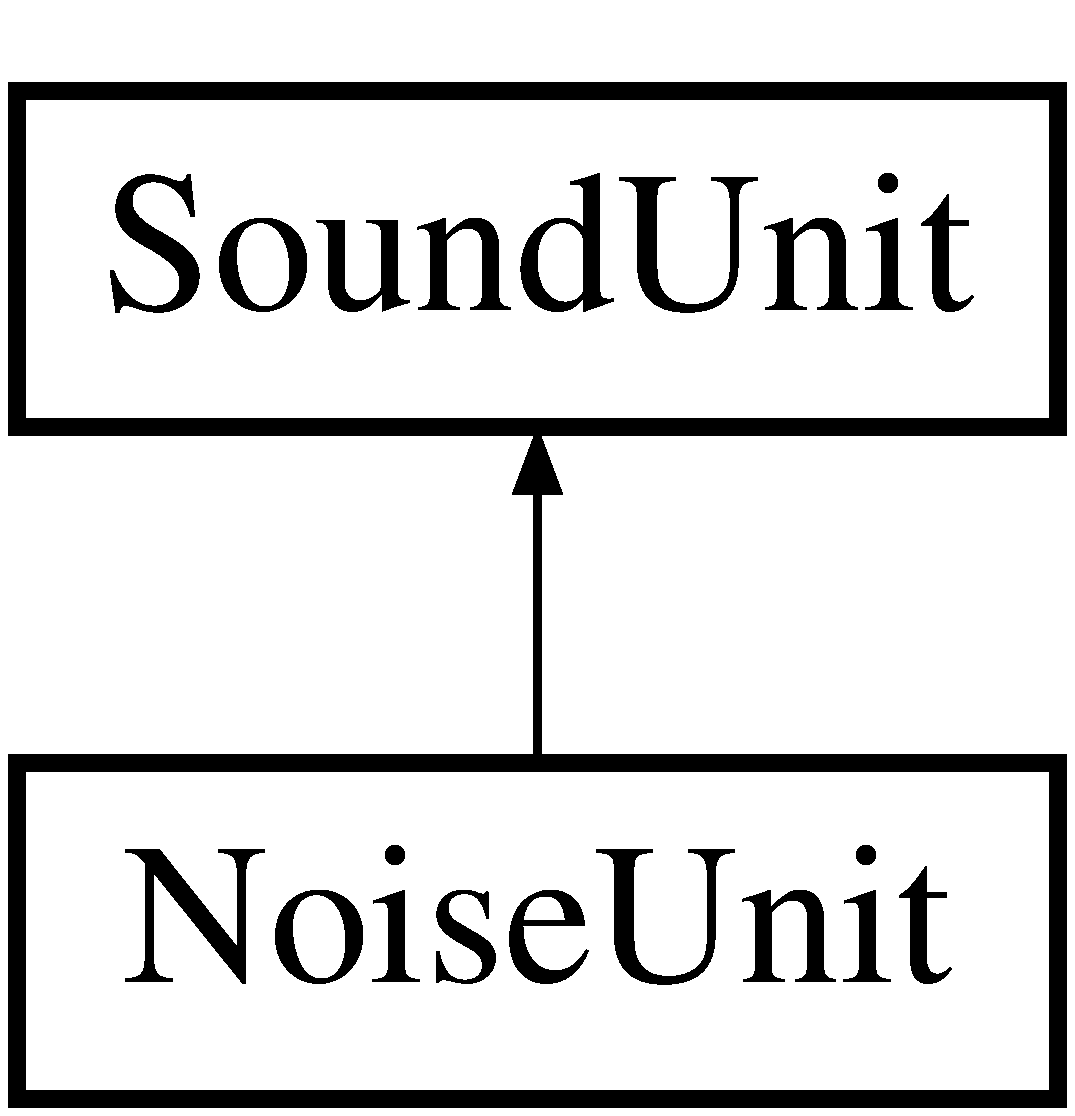
\includegraphics[height=2.000000cm]{classSoundUnit}
\end{center}
\end{figure}
\subsection*{Public Member Functions}
\begin{DoxyCompactItemize}
\item 
{\bfseries Sound\+Unit} (std\+::string name)\hypertarget{classSoundUnit_a3220665fe1e433d1b0d90fa328e71133}{}\label{classSoundUnit_a3220665fe1e433d1b0d90fa328e71133}

\item 
void {\bfseries add\+U\+Gen} (\hyperlink{classUGen}{U\+Gen} $\ast$u)\hypertarget{classSoundUnit_ab88bf7e7dfb77cf7e18587fd5a637755}{}\label{classSoundUnit_ab88bf7e7dfb77cf7e18587fd5a637755}

\item 
std\+::string {\bfseries get\+Name} ()\hypertarget{classSoundUnit_a4854dfb9b839ff33d061ed013fbf3ef9}{}\label{classSoundUnit_a4854dfb9b839ff33d061ed013fbf3ef9}

\item 
virtual void {\bfseries setup} ()=0\hypertarget{classSoundUnit_aedfa9b99f4555ed5df4ceffe001c1e63}{}\label{classSoundUnit_aedfa9b99f4555ed5df4ceffe001c1e63}

\item 
virtual void {\bfseries control} (std\+::string port\+Name, float value)=0\hypertarget{classSoundUnit_a0a74ef3d6c9343f1ee64a9a96bdbbe78}{}\label{classSoundUnit_a0a74ef3d6c9343f1ee64a9a96bdbbe78}

\item 
virtual float {\bfseries tick} ()=0\hypertarget{classSoundUnit_af1f6ccffb8d1919bd774b340c01bea68}{}\label{classSoundUnit_af1f6ccffb8d1919bd774b340c01bea68}

\end{DoxyCompactItemize}
\subsection*{Protected Attributes}
\begin{DoxyCompactItemize}
\item 
std\+::map$<$ std\+::string, \hyperlink{classUGen}{U\+Gen} $\ast$ $>$ {\bfseries U\+G\+E\+NS}\hypertarget{classSoundUnit_aa7bb4be0804fdd7a68bd767795592da1}{}\label{classSoundUnit_aa7bb4be0804fdd7a68bd767795592da1}

\end{DoxyCompactItemize}


The documentation for this class was generated from the following files\+:\begin{DoxyCompactItemize}
\item 
unit/Sound\+Unit.\+h\item 
unit/Sound\+Unit.\+cpp\end{DoxyCompactItemize}

\hypertarget{classunit_1_1SquareGen}{}\section{unit\+:\+:Square\+Gen Class Reference}
\label{classunit_1_1SquareGen}\index{unit\+::\+Square\+Gen@{unit\+::\+Square\+Gen}}
Inheritance diagram for unit\+:\+:Square\+Gen\+:\begin{figure}[H]
\begin{center}
\leavevmode
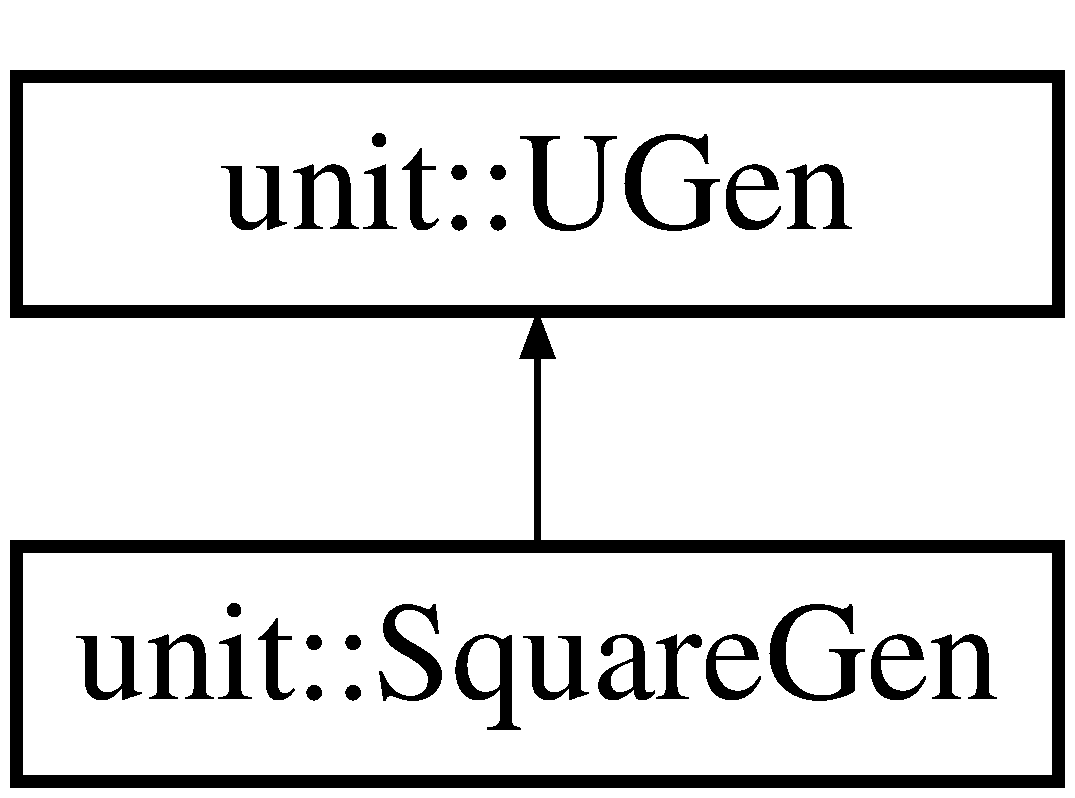
\includegraphics[height=2.000000cm]{classunit_1_1SquareGen}
\end{center}
\end{figure}
\subsection*{Public Member Functions}
\begin{DoxyCompactItemize}
\item 
{\bfseries Square\+Gen} (std\+::string name)\hypertarget{classunit_1_1SquareGen_a626505e8ade08b9383acda8901aa23b5}{}\label{classunit_1_1SquareGen_a626505e8ade08b9383acda8901aa23b5}

\item 
void {\bfseries control} (std\+::string port\+Name, float value)\hypertarget{classunit_1_1SquareGen_a8a25dc2b8c5d1ec7857e4da7ec96cecc}{}\label{classunit_1_1SquareGen_a8a25dc2b8c5d1ec7857e4da7ec96cecc}

\item 
float {\bfseries tick} ()\hypertarget{classunit_1_1SquareGen_a119ab47582ee5814687b87db6a71644c}{}\label{classunit_1_1SquareGen_a119ab47582ee5814687b87db6a71644c}

\end{DoxyCompactItemize}
\subsection*{Additional Inherited Members}


The documentation for this class was generated from the following files\+:\begin{DoxyCompactItemize}
\item 
unit/Square\+Gen.\+h\item 
unit/Square\+Gen.\+cpp\end{DoxyCompactItemize}

\hypertarget{classunit_1_1STKAdapterGen}{}\section{unit\+:\+:S\+T\+K\+Adapter\+Gen Class Reference}
\label{classunit_1_1STKAdapterGen}\index{unit\+::\+S\+T\+K\+Adapter\+Gen@{unit\+::\+S\+T\+K\+Adapter\+Gen}}


{\ttfamily \#include $<$S\+T\+K\+Adapter\+Gen.\+h$>$}

Inheritance diagram for unit\+:\+:S\+T\+K\+Adapter\+Gen\+:\begin{figure}[H]
\begin{center}
\leavevmode
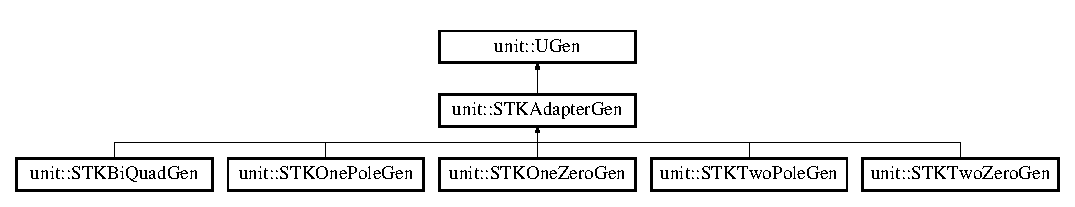
\includegraphics[height=2.333333cm]{classunit_1_1STKAdapterGen}
\end{center}
\end{figure}
\subsection*{Additional Inherited Members}


\subsection{Detailed Description}
\hyperlink{classunit_1_1STKAdapterGen}{S\+T\+K\+Adapter\+Gen} is an intermediate class and acts as a superclass to a number of S\+TK (Synthesis Tool Kit) functions.

To reduce depencies, the S\+TK functions will be replaced with equivalent \hyperlink{classNeonlicht}{Neonlicht} functions in the future.

\begin{DoxyAuthor}{Author}
jtm, email\+:  \href{mailto:milde@hs-fulda.de}{\tt milde@hs-\/fulda.\+de} 
\end{DoxyAuthor}
\begin{DoxySince}{Since}
04-\/2016 
\end{DoxySince}
\begin{DoxyVersion}{Version}
1.\+0 
\end{DoxyVersion}


The documentation for this class was generated from the following file\+:\begin{DoxyCompactItemize}
\item 
include/S\+T\+K\+Adapter\+Gen.\+h\end{DoxyCompactItemize}

\hypertarget{classunit_1_1STKBiQuadGen}{}\section{unit\+:\+:S\+T\+K\+Bi\+Quad\+Gen Class Reference}
\label{classunit_1_1STKBiQuadGen}\index{unit\+::\+S\+T\+K\+Bi\+Quad\+Gen@{unit\+::\+S\+T\+K\+Bi\+Quad\+Gen}}
Inheritance diagram for unit\+:\+:S\+T\+K\+Bi\+Quad\+Gen\+:\begin{figure}[H]
\begin{center}
\leavevmode
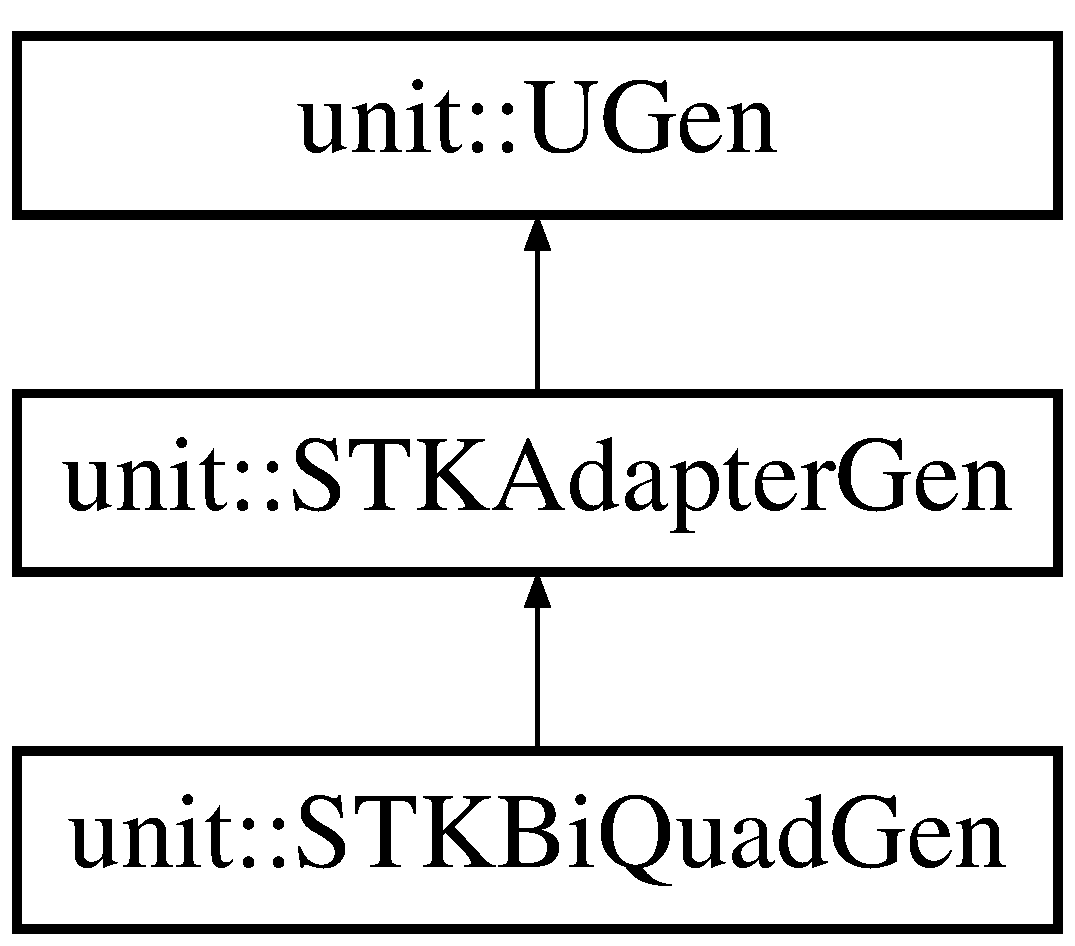
\includegraphics[height=3.000000cm]{classunit_1_1STKBiQuadGen}
\end{center}
\end{figure}
\subsection*{Public Member Functions}
\begin{DoxyCompactItemize}
\item 
void {\bfseries control} (std\+::string port\+Name, float value)\hypertarget{classunit_1_1STKBiQuadGen_afbaea4e23ab453fdeaa0069ddd8002a6}{}\label{classunit_1_1STKBiQuadGen_afbaea4e23ab453fdeaa0069ddd8002a6}

\item 
float {\bfseries tick} ()\hypertarget{classunit_1_1STKBiQuadGen_aeaa64c8ff587d9a9089b4cf3276255b9}{}\label{classunit_1_1STKBiQuadGen_aeaa64c8ff587d9a9089b4cf3276255b9}

\end{DoxyCompactItemize}
\subsection*{Additional Inherited Members}


The documentation for this class was generated from the following files\+:\begin{DoxyCompactItemize}
\item 
include/S\+T\+K\+Bi\+Quad\+Gen.\+h\item 
unit/S\+T\+K\+Bi\+Quad\+Gen.\+cpp\end{DoxyCompactItemize}

\hypertarget{classunit_1_1STKOnePoleGen}{\section{unit\-:\-:S\-T\-K\-One\-Pole\-Gen Class Reference}
\label{classunit_1_1STKOnePoleGen}\index{unit\-::\-S\-T\-K\-One\-Pole\-Gen@{unit\-::\-S\-T\-K\-One\-Pole\-Gen}}
}


{\ttfamily \#include $<$S\-T\-K\-One\-Pole\-Gen.\-h$>$}

Inheritance diagram for unit\-:\-:S\-T\-K\-One\-Pole\-Gen\-:\begin{figure}[H]
\begin{center}
\leavevmode
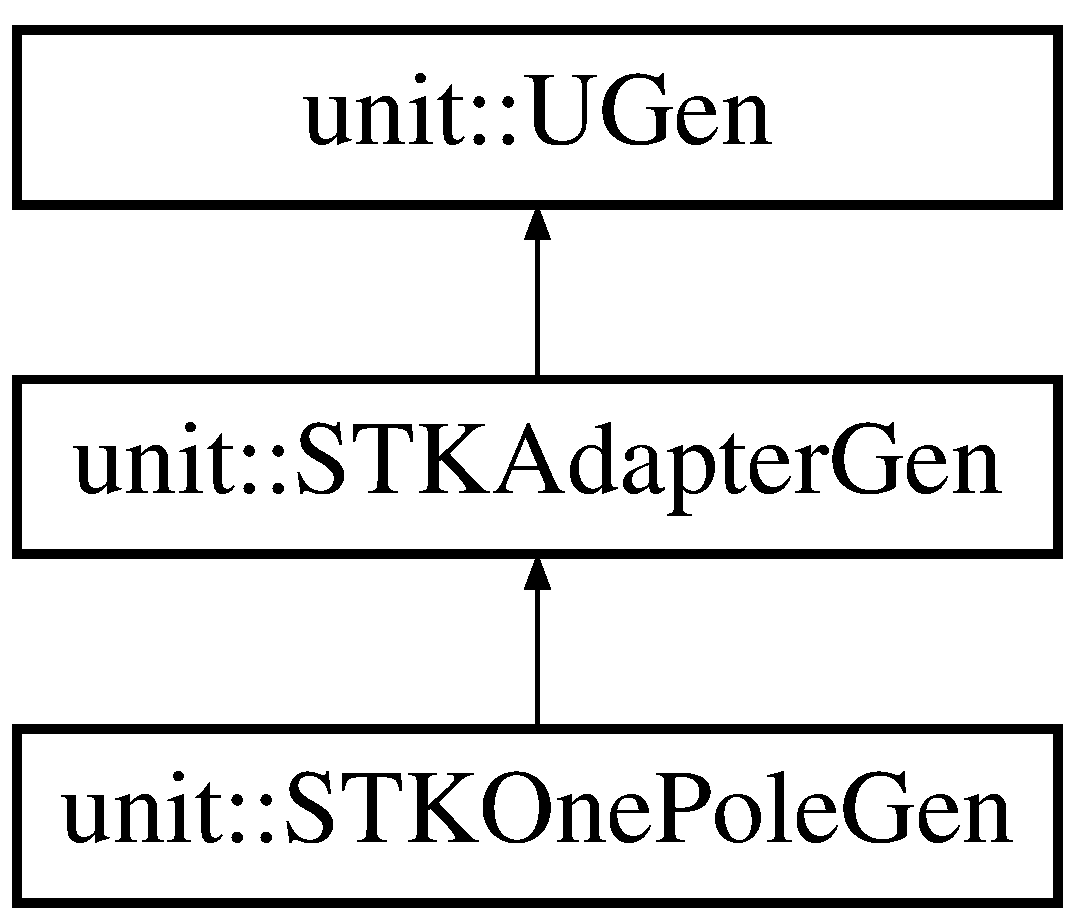
\includegraphics[height=3.000000cm]{classunit_1_1STKOnePoleGen}
\end{center}
\end{figure}
\subsection*{Public Member Functions}
\begin{DoxyCompactItemize}
\item 
\hypertarget{classunit_1_1STKOnePoleGen_abafc7a64770438cbde61518a7cf2d94b}{void {\bfseries control} (std\-::string port\-Name, float value)}\label{classunit_1_1STKOnePoleGen_abafc7a64770438cbde61518a7cf2d94b}

\item 
\hypertarget{classunit_1_1STKOnePoleGen_a3bc702fbc334d94eebd409755d1d74e8}{float {\bfseries tick} ()}\label{classunit_1_1STKOnePoleGen_a3bc702fbc334d94eebd409755d1d74e8}

\end{DoxyCompactItemize}
\subsection*{Additional Inherited Members}


\subsection{Detailed Description}
\hyperlink{classunit_1_1STKOnePoleGen}{S\-T\-K\-One\-Pole\-Gen} is an adapter to the One\-Pole filter of the S\-T\-K.

\begin{DoxyAuthor}{Author}
jtm, email\-:  \href{mailto:milde@hs-fulda.de}{\tt milde@hs-\/fulda.\-de} 
\end{DoxyAuthor}
\begin{DoxySince}{Since}
04-\/2016 
\end{DoxySince}
\begin{DoxyVersion}{Version}
1.\-0 
\end{DoxyVersion}


The documentation for this class was generated from the following files\-:\begin{DoxyCompactItemize}
\item 
src/include/S\-T\-K\-One\-Pole\-Gen.\-h\item 
src/unit/S\-T\-K\-One\-Pole\-Gen.\-cpp\end{DoxyCompactItemize}

\hypertarget{classunit_1_1STKOneZeroGen}{\section{unit\-:\-:S\-T\-K\-One\-Zero\-Gen Class Reference}
\label{classunit_1_1STKOneZeroGen}\index{unit\-::\-S\-T\-K\-One\-Zero\-Gen@{unit\-::\-S\-T\-K\-One\-Zero\-Gen}}
}


{\ttfamily \#include $<$S\-T\-K\-One\-Zero\-Gen.\-h$>$}

Inheritance diagram for unit\-:\-:S\-T\-K\-One\-Zero\-Gen\-:\begin{figure}[H]
\begin{center}
\leavevmode
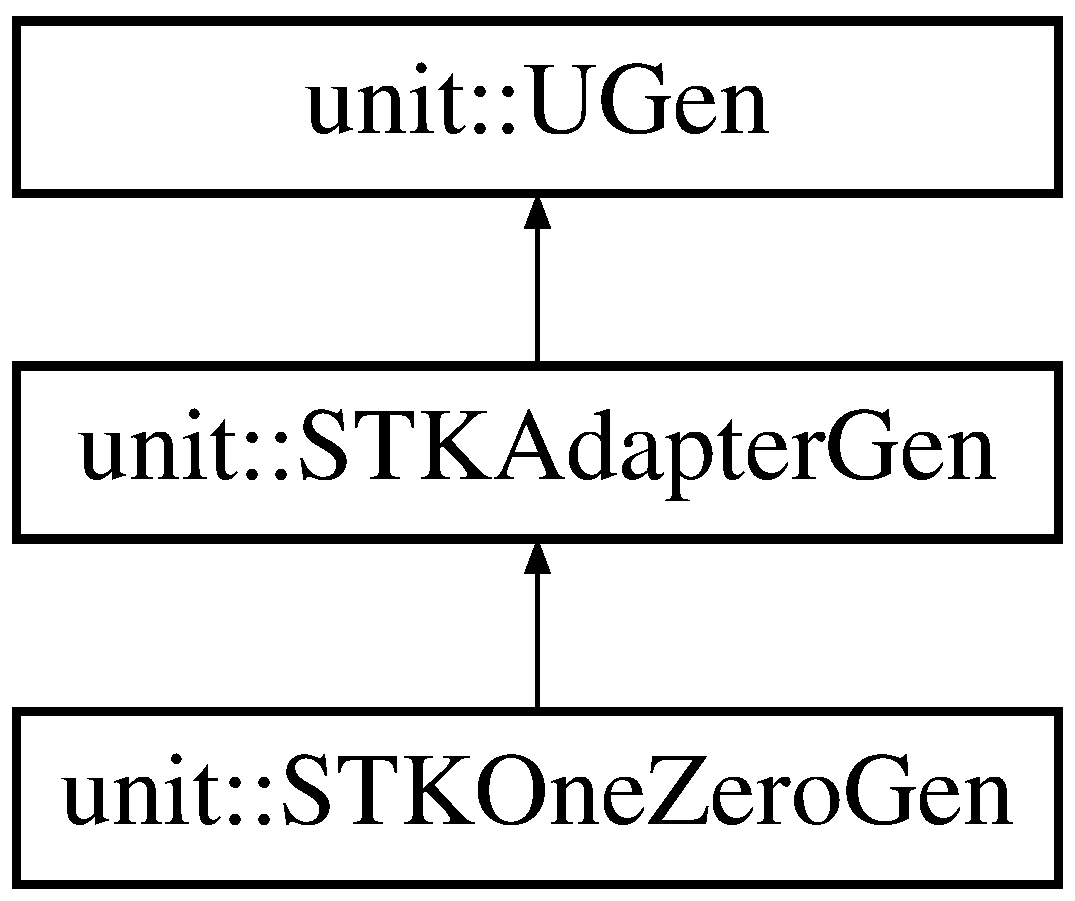
\includegraphics[height=3.000000cm]{classunit_1_1STKOneZeroGen}
\end{center}
\end{figure}
\subsection*{Public Member Functions}
\begin{DoxyCompactItemize}
\item 
\hypertarget{classunit_1_1STKOneZeroGen_a44bc26cf6f0e7218f9f14447c957dce4}{void {\bfseries control} (std\-::string port\-Name, float value)}\label{classunit_1_1STKOneZeroGen_a44bc26cf6f0e7218f9f14447c957dce4}

\item 
\hypertarget{classunit_1_1STKOneZeroGen_ab1118ea13c6892f49c8f92f017b82908}{float {\bfseries tick} ()}\label{classunit_1_1STKOneZeroGen_ab1118ea13c6892f49c8f92f017b82908}

\end{DoxyCompactItemize}
\subsection*{Additional Inherited Members}


\subsection{Detailed Description}
\hyperlink{classunit_1_1STKOneZeroGen}{S\-T\-K\-One\-Zero\-Gen} is an adapter to the One\-Zero filter of the S\-T\-K.

\begin{DoxyAuthor}{Author}
jtm, email\-:  \href{mailto:milde@hs-fulda.de}{\tt milde@hs-\/fulda.\-de} 
\end{DoxyAuthor}
\begin{DoxySince}{Since}
04-\/2016 
\end{DoxySince}
\begin{DoxyVersion}{Version}
1.\-0 
\end{DoxyVersion}


The documentation for this class was generated from the following files\-:\begin{DoxyCompactItemize}
\item 
include/S\-T\-K\-One\-Zero\-Gen.\-h\item 
unit/S\-T\-K\-One\-Zero\-Gen.\-cpp\end{DoxyCompactItemize}

\hypertarget{classunit_1_1STKTwoPoleGen}{\section{unit\-:\-:S\-T\-K\-Two\-Pole\-Gen Class Reference}
\label{classunit_1_1STKTwoPoleGen}\index{unit\-::\-S\-T\-K\-Two\-Pole\-Gen@{unit\-::\-S\-T\-K\-Two\-Pole\-Gen}}
}


{\ttfamily \#include $<$S\-T\-K\-Two\-Pole\-Gen.\-h$>$}

Inheritance diagram for unit\-:\-:S\-T\-K\-Two\-Pole\-Gen\-:\begin{figure}[H]
\begin{center}
\leavevmode
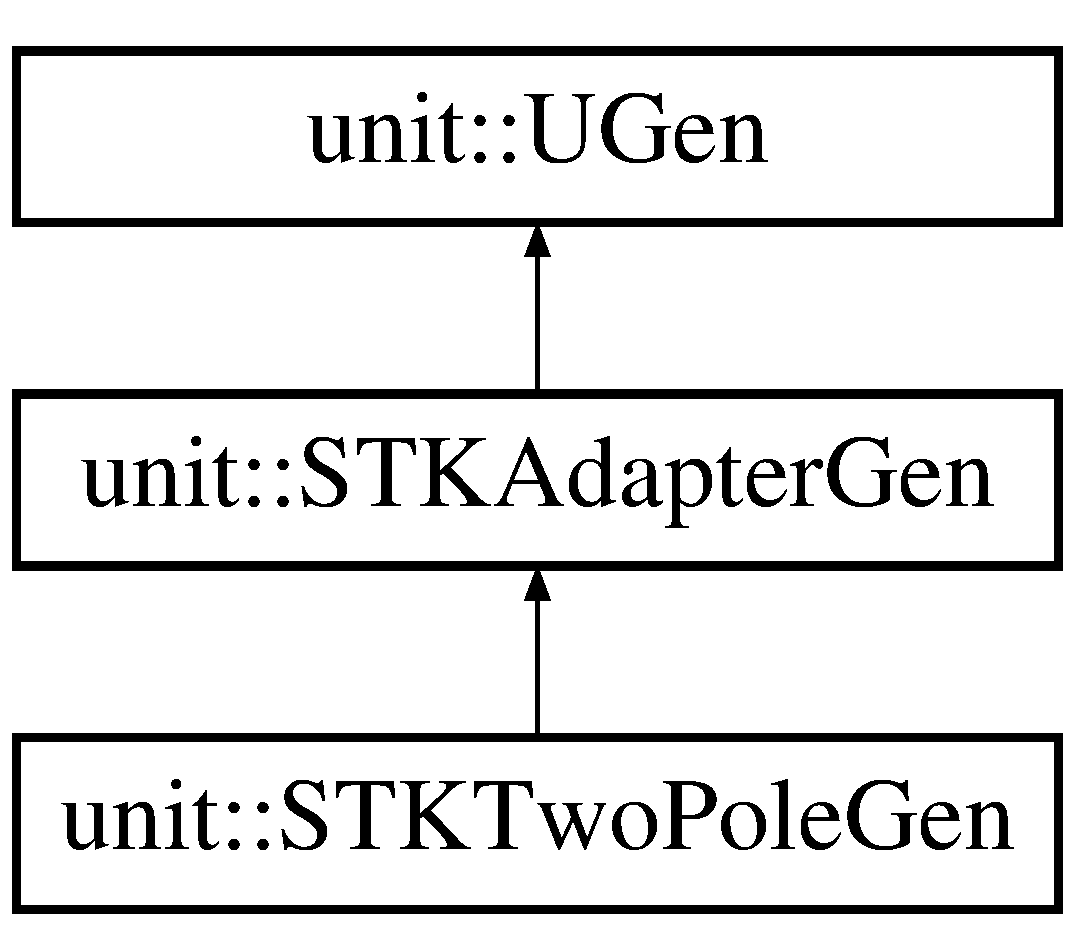
\includegraphics[height=3.000000cm]{classunit_1_1STKTwoPoleGen}
\end{center}
\end{figure}
\subsection*{Public Member Functions}
\begin{DoxyCompactItemize}
\item 
\hypertarget{classunit_1_1STKTwoPoleGen_a71b904b3c03c69f5fb25bbf2449fb802}{void {\bfseries control} (std\-::string port\-Name, float value)}\label{classunit_1_1STKTwoPoleGen_a71b904b3c03c69f5fb25bbf2449fb802}

\item 
\hypertarget{classunit_1_1STKTwoPoleGen_ade033932ab7e85b7f3d6a69461eef372}{float {\bfseries tick} ()}\label{classunit_1_1STKTwoPoleGen_ade033932ab7e85b7f3d6a69461eef372}

\end{DoxyCompactItemize}
\subsection*{Additional Inherited Members}


\subsection{Detailed Description}
\hyperlink{classunit_1_1STKTwoPoleGen}{S\-T\-K\-Two\-Pole\-Gen} is an adapter to the Two\-Pole filter of the S\-T\-K.

\begin{DoxyAuthor}{Author}
jtm, email\-:  \href{mailto:milde@hs-fulda.de}{\tt milde@hs-\/fulda.\-de} 
\end{DoxyAuthor}
\begin{DoxySince}{Since}
04-\/2016 
\end{DoxySince}
\begin{DoxyVersion}{Version}
1.\-0 
\end{DoxyVersion}


The documentation for this class was generated from the following files\-:\begin{DoxyCompactItemize}
\item 
src/include/S\-T\-K\-Two\-Pole\-Gen.\-h\item 
src/unit/S\-T\-K\-Two\-Pole\-Gen.\-cpp\end{DoxyCompactItemize}

\hypertarget{classunit_1_1STKTwoZeroGen}{}\section{unit\+:\+:S\+T\+K\+Two\+Zero\+Gen Class Reference}
\label{classunit_1_1STKTwoZeroGen}\index{unit\+::\+S\+T\+K\+Two\+Zero\+Gen@{unit\+::\+S\+T\+K\+Two\+Zero\+Gen}}
Inheritance diagram for unit\+:\+:S\+T\+K\+Two\+Zero\+Gen\+:\begin{figure}[H]
\begin{center}
\leavevmode
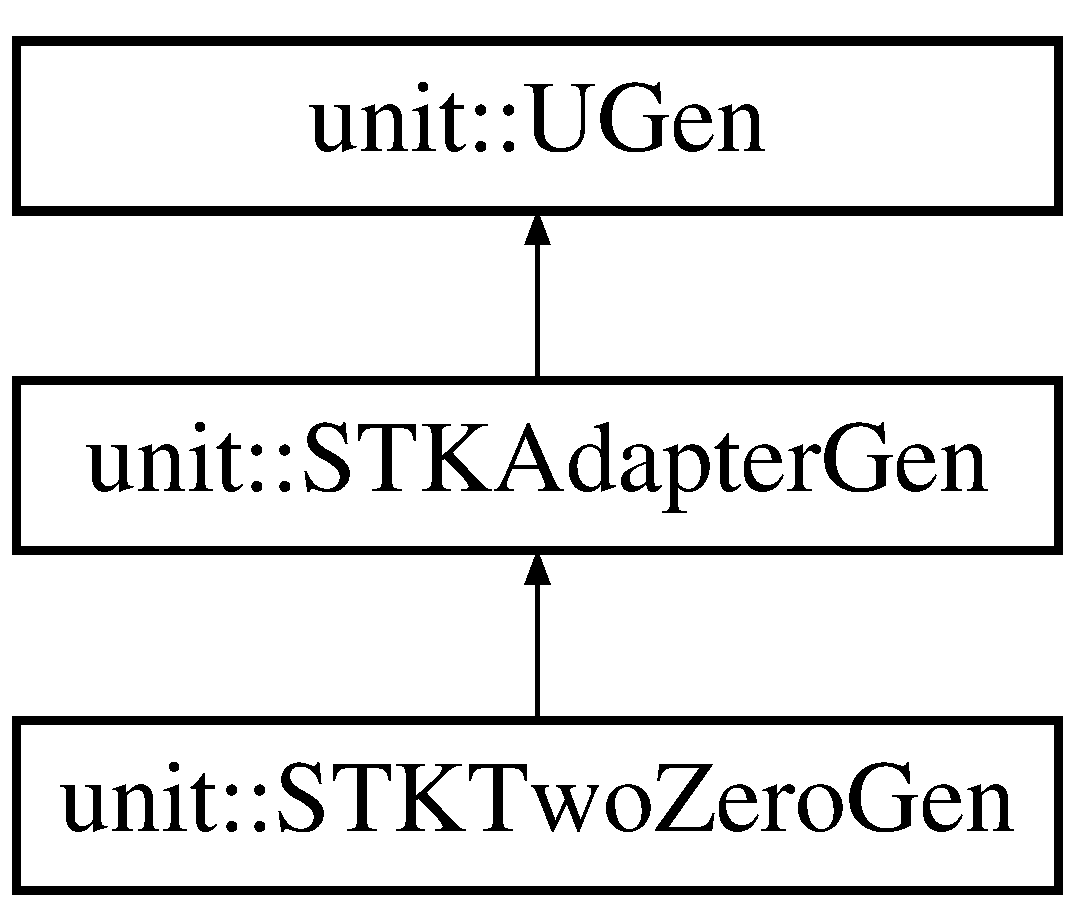
\includegraphics[height=3.000000cm]{classunit_1_1STKTwoZeroGen}
\end{center}
\end{figure}
\subsection*{Public Member Functions}
\begin{DoxyCompactItemize}
\item 
void {\bfseries control} (std\+::string port\+Name, float value)\hypertarget{classunit_1_1STKTwoZeroGen_a35f0458e31142985a3f35b603ff90e62}{}\label{classunit_1_1STKTwoZeroGen_a35f0458e31142985a3f35b603ff90e62}

\item 
float {\bfseries tick} ()\hypertarget{classunit_1_1STKTwoZeroGen_a1e9392a2e8dc67862de802e914acbf33}{}\label{classunit_1_1STKTwoZeroGen_a1e9392a2e8dc67862de802e914acbf33}

\end{DoxyCompactItemize}
\subsection*{Additional Inherited Members}


The documentation for this class was generated from the following files\+:\begin{DoxyCompactItemize}
\item 
unit/S\+T\+K\+Two\+Zero\+Gen.\+h\item 
unit/S\+T\+K\+Two\+Zero\+Gen.\+cpp\end{DoxyCompactItemize}

\hypertarget{classTestStatic}{\section{Test\-Static Class Reference}
\label{classTestStatic}\index{Test\-Static@{Test\-Static}}
}
\subsection*{Public Member Functions}
\begin{DoxyCompactItemize}
\item 
\hypertarget{classTestStatic_af877b62beba36ec427f5a20cf0b261e5}{void {\bfseries printit} ()}\label{classTestStatic_af877b62beba36ec427f5a20cf0b261e5}

\end{DoxyCompactItemize}
\subsection*{Static Public Member Functions}
\begin{DoxyCompactItemize}
\item 
\hypertarget{classTestStatic_af09e079b702a6fba0a9623c136665d90}{static void {\bfseries do\-Something} (int val)}\label{classTestStatic_af09e079b702a6fba0a9623c136665d90}

\end{DoxyCompactItemize}


The documentation for this class was generated from the following files\-:\begin{DoxyCompactItemize}
\item 
src/outdated/Test\-Static.\-h\item 
src/outdated/Test\-Static.\-cpp\end{DoxyCompactItemize}

\hypertarget{structTickData}{\section{Tick\-Data Struct Reference}
\label{structTickData}\index{Tick\-Data@{Tick\-Data}}
}
\subsection*{Public Attributes}
\begin{DoxyCompactItemize}
\item 
\hypertarget{structTickData_a81bc42e25163a7afb9725153fac3d713}{stk\-::\-Stk\-Float {\bfseries volume}}\label{structTickData_a81bc42e25163a7afb9725153fac3d713}

\item 
\hypertarget{structTickData_a9916301f9f675256327e1ac0bdb8f9f4}{stk\-::\-Stk\-Float {\bfseries t60}}\label{structTickData_a9916301f9f675256327e1ac0bdb8f9f4}

\item 
\hypertarget{structTickData_abda86f5671f18f3e09fa6e0877c70bca}{unsigned int {\bfseries n\-Wv\-Outs}}\label{structTickData_abda86f5671f18f3e09fa6e0877c70bca}

\item 
\hypertarget{structTickData_ac53a7ecd6dfff24019bfb607202f6024}{int {\bfseries n\-Voices}}\label{structTickData_ac53a7ecd6dfff24019bfb607202f6024}

\item 
\hypertarget{structTickData_a620ca81cff77e4cdaf0025b73bc37e61}{int {\bfseries current\-Voice}}\label{structTickData_a620ca81cff77e4cdaf0025b73bc37e61}

\item 
\hypertarget{structTickData_ad147869433dc1b3526aa9f4dbb3b4cc5}{int {\bfseries channels}}\label{structTickData_ad147869433dc1b3526aa9f4dbb3b4cc5}

\item 
\hypertarget{structTickData_a54ba17f6bb83ce8efe0758614221f026}{int {\bfseries counter}}\label{structTickData_a54ba17f6bb83ce8efe0758614221f026}

\item 
\hypertarget{structTickData_aa60016ecb88b0bdae8395aa7517a6f1f}{bool {\bfseries realtime}}\label{structTickData_aa60016ecb88b0bdae8395aa7517a6f1f}

\item 
\hypertarget{structTickData_a4682f375c65eb79d9166933ec9c79c2b}{bool {\bfseries settling}}\label{structTickData_a4682f375c65eb79d9166933ec9c79c2b}

\item 
\hypertarget{structTickData_a142d947db0ab6e66f8f912c51a4bafdb}{bool {\bfseries have\-Message}}\label{structTickData_a142d947db0ab6e66f8f912c51a4bafdb}

\item 
\hypertarget{structTickData_ade8d551a52ad93b8f056bf5da813c64c}{int {\bfseries frequency}}\label{structTickData_ade8d551a52ad93b8f056bf5da813c64c}

\item 
\hypertarget{structTickData_a99559444aee6dbc126f650744c5487ec}{Wv\-Out $\ast$$\ast$ {\bfseries wvout}}\label{structTickData_a99559444aee6dbc126f650744c5487ec}

\item 
\hypertarget{structTickData_aa2b6f7f6ad9c886711e9393aca979677}{Instrmnt $\ast$$\ast$ {\bfseries instrument}}\label{structTickData_aa2b6f7f6ad9c886711e9393aca979677}

\item 
\hypertarget{structTickData_ade98160894388bc8534d2003a7a63ffe}{Voicer $\ast$ {\bfseries voicer}}\label{structTickData_ade98160894388bc8534d2003a7a63ffe}

\item 
\hypertarget{structTickData_a3d1563b3668509206700be3e02138827}{J\-C\-Rev {\bfseries reverb}}\label{structTickData_a3d1563b3668509206700be3e02138827}

\item 
\hypertarget{structTickData_a3d0c2a9deef2fd2bd94b3ba8c6b176eb}{Messager {\bfseries messager}}\label{structTickData_a3d0c2a9deef2fd2bd94b3ba8c6b176eb}

\item 
\hypertarget{structTickData_a3061482937dae6c292d4d51400a6143a}{Skini\-::\-Message {\bfseries message}}\label{structTickData_a3061482937dae6c292d4d51400a6143a}

\item 
\hypertarget{structTickData_a6d0680a0bcc9d2c35104ad9721777223}{Stk\-Float {\bfseries volume}}\label{structTickData_a6d0680a0bcc9d2c35104ad9721777223}

\item 
\hypertarget{structTickData_adf8ffe69c6880e995aec842a032ee9fe}{Stk\-Float {\bfseries t60}}\label{structTickData_adf8ffe69c6880e995aec842a032ee9fe}

\end{DoxyCompactItemize}


The documentation for this struct was generated from the following files\-:\begin{DoxyCompactItemize}
\item 
include/Tick\-Data.\-h\item 
outdated/first.\-cpp\end{DoxyCompactItemize}

\hypertarget{classunit_1_1TwoInputMixerGen}{}\section{unit\+:\+:Two\+Input\+Mixer\+Gen Class Reference}
\label{classunit_1_1TwoInputMixerGen}\index{unit\+::\+Two\+Input\+Mixer\+Gen@{unit\+::\+Two\+Input\+Mixer\+Gen}}
Inheritance diagram for unit\+:\+:Two\+Input\+Mixer\+Gen\+:\begin{figure}[H]
\begin{center}
\leavevmode
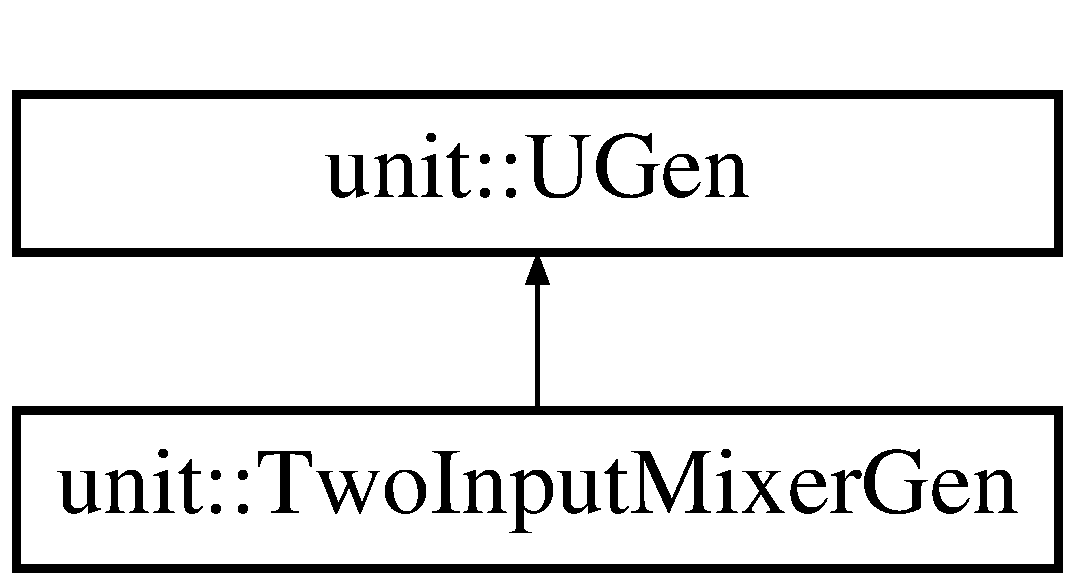
\includegraphics[height=2.000000cm]{classunit_1_1TwoInputMixerGen}
\end{center}
\end{figure}
\subsection*{Public Member Functions}
\begin{DoxyCompactItemize}
\item 
{\bfseries Two\+Input\+Mixer\+Gen} (std\+::string name)\hypertarget{classunit_1_1TwoInputMixerGen_ae150f51a934ffb7330f8a2852b094539}{}\label{classunit_1_1TwoInputMixerGen_ae150f51a934ffb7330f8a2852b094539}

\item 
float {\bfseries tick} ()\hypertarget{classunit_1_1TwoInputMixerGen_aef96ef6828e767384a8881d108c0d52b}{}\label{classunit_1_1TwoInputMixerGen_aef96ef6828e767384a8881d108c0d52b}

\item 
void {\bfseries control} (std\+::string port\+Name, float value)\hypertarget{classunit_1_1TwoInputMixerGen_ab8d7d00eb0c692a8c2de706f58673d3d}{}\label{classunit_1_1TwoInputMixerGen_ab8d7d00eb0c692a8c2de706f58673d3d}

\end{DoxyCompactItemize}
\subsection*{Additional Inherited Members}


The documentation for this class was generated from the following files\+:\begin{DoxyCompactItemize}
\item 
include/Two\+Input\+Mixer\+Gen.\+h\item 
unit/Two\+Input\+Mixer\+Gen.\+cpp\end{DoxyCompactItemize}

\hypertarget{classunit_1_1UGen}{}\section{unit\+:\+:U\+Gen Class Reference}
\label{classunit_1_1UGen}\index{unit\+::\+U\+Gen@{unit\+::\+U\+Gen}}


{\ttfamily \#include $<$U\+Gen.\+h$>$}

Inheritance diagram for unit\+:\+:U\+Gen\+:\begin{figure}[H]
\begin{center}
\leavevmode
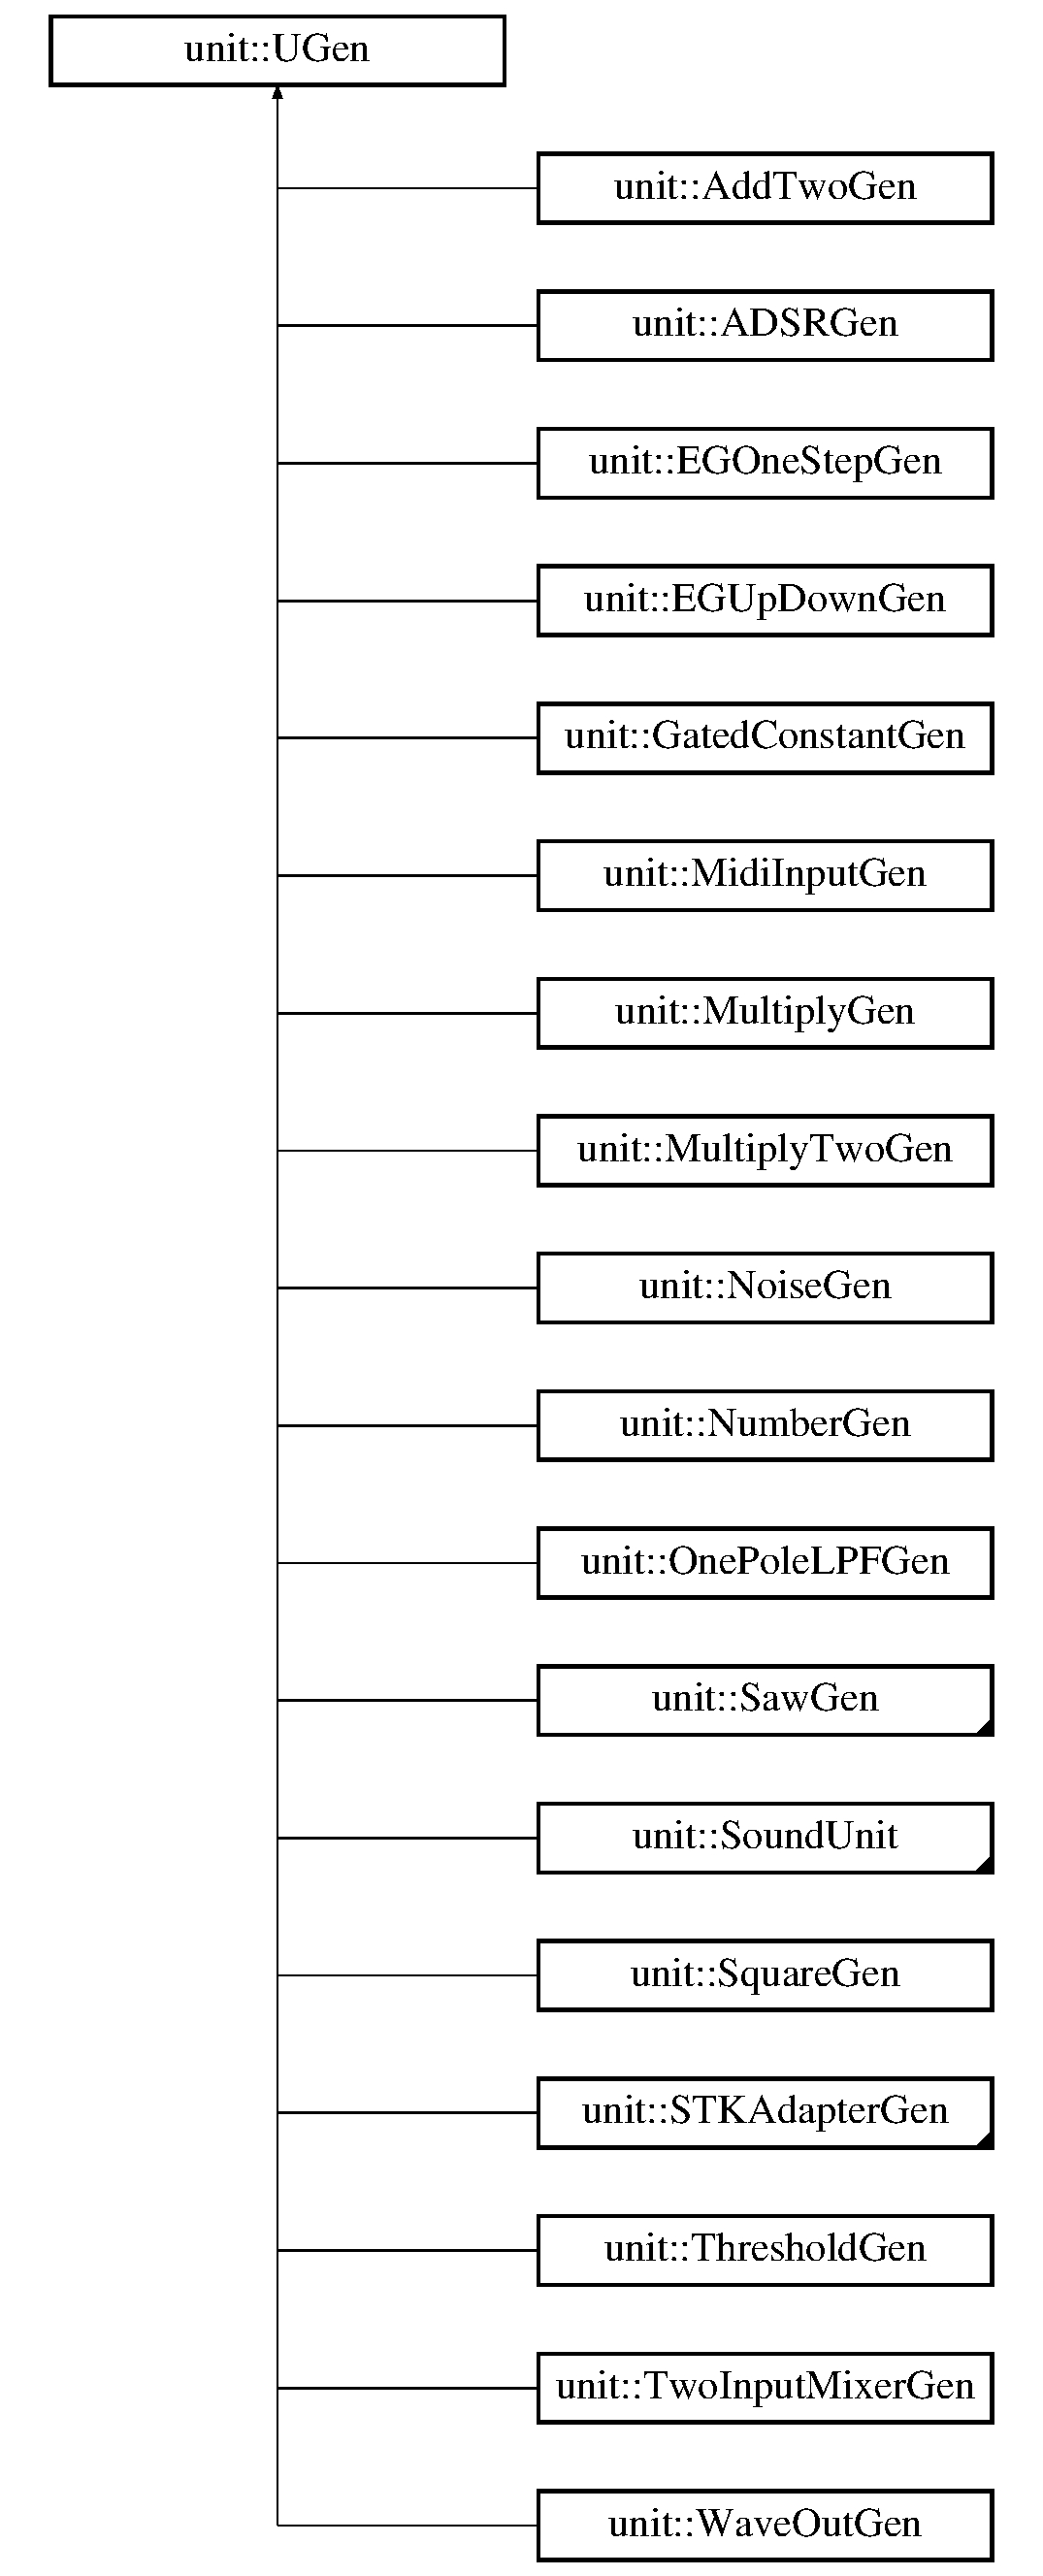
\includegraphics[height=12.000000cm]{classunit_1_1UGen}
\end{center}
\end{figure}
\subsection*{Public Member Functions}
\begin{DoxyCompactItemize}
\item 
{\bfseries U\+Gen} (std\+::string name, int pn)\hypertarget{classunit_1_1UGen_af2d6d70e1340c9853a9a329cb2db164a}{}\label{classunit_1_1UGen_af2d6d70e1340c9853a9a329cb2db164a}

\item 
void {\bfseries add\+Port} (\hyperlink{classPort}{Port} p)\hypertarget{classunit_1_1UGen_a7d5be76c0847cea2ffd9fb6118dad84b}{}\label{classunit_1_1UGen_a7d5be76c0847cea2ffd9fb6118dad84b}

\item 
\hyperlink{classPort}{Port} $\ast$ {\bfseries get\+Ports} ()\hypertarget{classunit_1_1UGen_a2dbed70294dba960bebb4e6e6196f93f}{}\label{classunit_1_1UGen_a2dbed70294dba960bebb4e6e6196f93f}

\item 
int {\bfseries get\+Number\+Of\+Ports} ()\hypertarget{classunit_1_1UGen_a1f7c0151b63c89a92ea7b3b598969fb5}{}\label{classunit_1_1UGen_a1f7c0151b63c89a92ea7b3b598969fb5}

\item 
float {\bfseries get\+Port\+Value} (int pn)\hypertarget{classunit_1_1UGen_a5790d6f5f741d9286e12f27eafd86bd5}{}\label{classunit_1_1UGen_a5790d6f5f741d9286e12f27eafd86bd5}

\item 
float {\bfseries get\+Port\+Value} (std\+::string name)\hypertarget{classunit_1_1UGen_a2a33803a853db61cc79cc6da90ce511d}{}\label{classunit_1_1UGen_a2a33803a853db61cc79cc6da90ce511d}

\item 
void {\bfseries set\+Port\+Value} (int pn, float value)\hypertarget{classunit_1_1UGen_ae933825c4201f13cb481d399de1bd4d5}{}\label{classunit_1_1UGen_ae933825c4201f13cb481d399de1bd4d5}

\item 
void {\bfseries set\+Port\+Value} (std\+::string name, float value)\hypertarget{classunit_1_1UGen_a1ed212c207052705c9fbd2fb64fe1092}{}\label{classunit_1_1UGen_a1ed212c207052705c9fbd2fb64fe1092}

\item 
int {\bfseries get\+Port\+Index} (std\+::string id)\hypertarget{classunit_1_1UGen_a7caac30e931fe2e39c53be9a084e2709}{}\label{classunit_1_1UGen_a7caac30e931fe2e39c53be9a084e2709}

\item 
std\+::string {\bfseries get\+Name} ()\hypertarget{classunit_1_1UGen_adfb82e003597ca4876f803f0395b28d6}{}\label{classunit_1_1UGen_adfb82e003597ca4876f803f0395b28d6}

\item 
std\+::string {\bfseries get\+ID} ()\hypertarget{classunit_1_1UGen_a500ba300703167f4daa52b51841edf24}{}\label{classunit_1_1UGen_a500ba300703167f4daa52b51841edf24}

\item 
virtual void {\bfseries control} (std\+::string port\+Name, float value)\hypertarget{classunit_1_1UGen_a456a55e23a073bc77135525be38ad0eb}{}\label{classunit_1_1UGen_a456a55e23a073bc77135525be38ad0eb}

\item 
virtual float {\bfseries tick} ()\hypertarget{classunit_1_1UGen_a7fe124a01b35094197816cb8aa033c55}{}\label{classunit_1_1UGen_a7fe124a01b35094197816cb8aa033c55}

\item 
void {\bfseries set\+Amnt1} (float value)\hypertarget{classunit_1_1UGen_a5063e6854f054cf7870abf1fdcbf8e30}{}\label{classunit_1_1UGen_a5063e6854f054cf7870abf1fdcbf8e30}

\item 
float {\bfseries get\+Amnt1} ()\hypertarget{classunit_1_1UGen_a98614bdc04b7c096fa7a75e486898947}{}\label{classunit_1_1UGen_a98614bdc04b7c096fa7a75e486898947}

\item 
void {\bfseries set\+Amnt2} (float value)\hypertarget{classunit_1_1UGen_a13494a4d13ad1fd32d16d5d22c22fb6d}{}\label{classunit_1_1UGen_a13494a4d13ad1fd32d16d5d22c22fb6d}

\item 
float {\bfseries get\+Amnt2} ()\hypertarget{classunit_1_1UGen_aa051f663b3fd0568eae2cad11b69058c}{}\label{classunit_1_1UGen_aa051f663b3fd0568eae2cad11b69058c}

\item 
void {\bfseries set\+Amnt3} (float value)\hypertarget{classunit_1_1UGen_aad0a3b7250c400216930062d651a1cf4}{}\label{classunit_1_1UGen_aad0a3b7250c400216930062d651a1cf4}

\item 
float {\bfseries get\+Amnt3} ()\hypertarget{classunit_1_1UGen_ac884f3a8cd1886698a9e2745940b9e1a}{}\label{classunit_1_1UGen_ac884f3a8cd1886698a9e2745940b9e1a}

\item 
void {\bfseries set\+In1} (float value)\hypertarget{classunit_1_1UGen_a4c68a850f5a690e39fd3903e52da313a}{}\label{classunit_1_1UGen_a4c68a850f5a690e39fd3903e52da313a}

\item 
float {\bfseries get\+In1} ()\hypertarget{classunit_1_1UGen_af1f157f807936bd22e201c9fa67ff80e}{}\label{classunit_1_1UGen_af1f157f807936bd22e201c9fa67ff80e}

\item 
void {\bfseries set\+In2} (float value)\hypertarget{classunit_1_1UGen_af3307a09f1ccefb80804f85edc9e305d}{}\label{classunit_1_1UGen_af3307a09f1ccefb80804f85edc9e305d}

\item 
float {\bfseries get\+In2} ()\hypertarget{classunit_1_1UGen_a9860c88b35b1d9e66559501f196a861c}{}\label{classunit_1_1UGen_a9860c88b35b1d9e66559501f196a861c}

\item 
void {\bfseries set\+Out1} (float value)\hypertarget{classunit_1_1UGen_ad1746a0b6380906d0d4a004e5c169247}{}\label{classunit_1_1UGen_ad1746a0b6380906d0d4a004e5c169247}

\item 
float {\bfseries get\+Out1} ()\hypertarget{classunit_1_1UGen_a71c193b988474251015828825e7cb49e}{}\label{classunit_1_1UGen_a71c193b988474251015828825e7cb49e}

\item 
void {\bfseries set\+Out2} (float value)\hypertarget{classunit_1_1UGen_af23d4016474b7d88cbbb6ed6660a10db}{}\label{classunit_1_1UGen_af23d4016474b7d88cbbb6ed6660a10db}

\item 
float {\bfseries get\+Out2} ()\hypertarget{classunit_1_1UGen_a37c67120e26ba5eef873e3ceb775eea0}{}\label{classunit_1_1UGen_a37c67120e26ba5eef873e3ceb775eea0}

\end{DoxyCompactItemize}
\subsection*{Protected Attributes}
\begin{DoxyCompactItemize}
\item 
float {\bfseries S\+A\+M\+P\+L\+I\+N\+G\+\_\+\+F\+R\+E\+Q\+U\+E\+N\+CY} = 44100\hypertarget{classunit_1_1UGen_af570ad383b680b2c79209b6ab28d010d}{}\label{classunit_1_1UGen_af570ad383b680b2c79209b6ab28d010d}

\item 
float {\bfseries amnt1}\hypertarget{classunit_1_1UGen_a4691cf88e3711c22617c11fc3ea3848e}{}\label{classunit_1_1UGen_a4691cf88e3711c22617c11fc3ea3848e}

\item 
float {\bfseries amnt2}\hypertarget{classunit_1_1UGen_a5e71a2e764029b4909c7e8535922e4b3}{}\label{classunit_1_1UGen_a5e71a2e764029b4909c7e8535922e4b3}

\item 
float {\bfseries amnt3}\hypertarget{classunit_1_1UGen_a14ebb8261a700f961c2d7808609470fe}{}\label{classunit_1_1UGen_a14ebb8261a700f961c2d7808609470fe}

\item 
float {\bfseries in1}\hypertarget{classunit_1_1UGen_aaf1873ae9668c6f1b37cae635bd40037}{}\label{classunit_1_1UGen_aaf1873ae9668c6f1b37cae635bd40037}

\item 
float {\bfseries in2}\hypertarget{classunit_1_1UGen_aed559bb431c46fe308560bd81756d169}{}\label{classunit_1_1UGen_aed559bb431c46fe308560bd81756d169}

\item 
float {\bfseries out1}\hypertarget{classunit_1_1UGen_a90ba3b9008a6d8386035db3dee502217}{}\label{classunit_1_1UGen_a90ba3b9008a6d8386035db3dee502217}

\item 
float {\bfseries out2}\hypertarget{classunit_1_1UGen_a779961bf3971a9f4c85d292dbb6d6d78}{}\label{classunit_1_1UGen_a779961bf3971a9f4c85d292dbb6d6d78}

\item 
std\+::string {\bfseries N\+A\+ME}\hypertarget{classunit_1_1UGen_ae468f7e763da88da4389b8bdbc306459}{}\label{classunit_1_1UGen_ae468f7e763da88da4389b8bdbc306459}

\item 
std\+::string {\bfseries ID}\hypertarget{classunit_1_1UGen_ab8d5acd179e175cc787ac43a49b68c29}{}\label{classunit_1_1UGen_ab8d5acd179e175cc787ac43a49b68c29}

\end{DoxyCompactItemize}


\subsection{Detailed Description}
\hyperlink{classunit_1_1UGen}{U\+Gen} is the base class for all Unit Generators. It provides the underlying interface of the U\+Gens. Two methods have to be implemented by the U\+Gens\+:

void control(std\+::string port\+Name, float value) is used to set port values of the \hyperlink{classunit_1_1UGen}{U\+Gen}. The user has to dispatch the port\+Name, no automatic dispatching is available (due to performance issues!)

float tick() is used to calculate the next output sample of the \hyperlink{classunit_1_1UGen}{U\+Gen}. Here the actual signal processing takes places. The user has to take care of input and output of the \hyperlink{classunit_1_1UGen}{U\+Gen}.

The default implmentation of \hyperlink{classunit_1_1UGen}{U\+Gen} provides three value ports (amnt1, amnt2, amnt3), two in ports (in1 and in2) and two out ports (out1 and out2). For these ports appropiate getter and setter methods are provided. The user may implement more ports, if needed for the functionality of the \hyperlink{classunit_1_1UGen}{U\+Gen}.

\begin{DoxyAuthor}{Author}
jtm 
\end{DoxyAuthor}
\begin{DoxySince}{Since}
04-\/2016 
\end{DoxySince}
\begin{DoxyVersion}{Version}
1.\+0 
\end{DoxyVersion}


The documentation for this class was generated from the following files\+:\begin{DoxyCompactItemize}
\item 
unit/U\+Gen.\+h\item 
unit/U\+Gen.\+cpp\end{DoxyCompactItemize}

\hypertarget{classunit_1_1WaveOutGen}{}\section{unit\+:\+:Wave\+Out\+Gen Class Reference}
\label{classunit_1_1WaveOutGen}\index{unit\+::\+Wave\+Out\+Gen@{unit\+::\+Wave\+Out\+Gen}}
Inheritance diagram for unit\+:\+:Wave\+Out\+Gen\+:\begin{figure}[H]
\begin{center}
\leavevmode
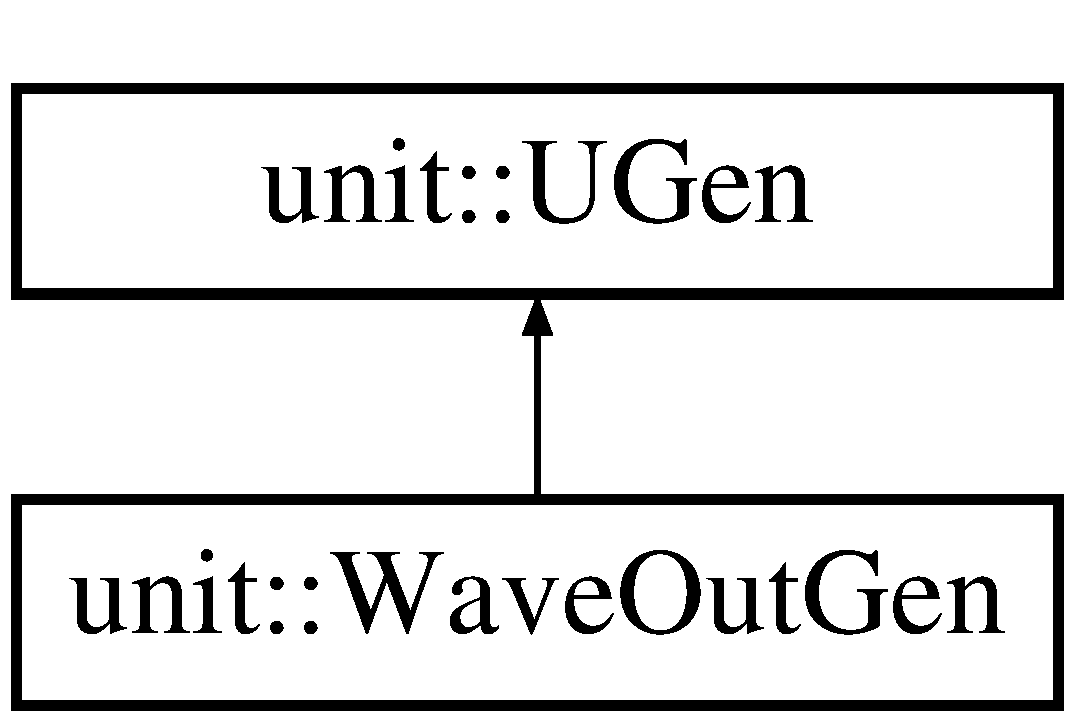
\includegraphics[height=2.000000cm]{classunit_1_1WaveOutGen}
\end{center}
\end{figure}
\subsection*{Public Member Functions}
\begin{DoxyCompactItemize}
\item 
{\bfseries Wave\+Out\+Gen} (std\+::string name)\hypertarget{classunit_1_1WaveOutGen_af7b0343212eb3de1ed4ef2dad90ad43e}{}\label{classunit_1_1WaveOutGen_af7b0343212eb3de1ed4ef2dad90ad43e}

\item 
void {\bfseries control} (std\+::string port\+Name, float value)\hypertarget{classunit_1_1WaveOutGen_a919d71ae0729553b3bd1799add9d1088}{}\label{classunit_1_1WaveOutGen_a919d71ae0729553b3bd1799add9d1088}

\item 
float {\bfseries tick} ()\hypertarget{classunit_1_1WaveOutGen_a468581d97aaf471e6516aee2cdb630cd}{}\label{classunit_1_1WaveOutGen_a468581d97aaf471e6516aee2cdb630cd}

\end{DoxyCompactItemize}
\subsection*{Public Attributes}
\begin{DoxyCompactItemize}
\item 
long {\bfseries count} = 0\hypertarget{classunit_1_1WaveOutGen_ad8ec171f5fa4fabc328b69a2509fde0f}{}\label{classunit_1_1WaveOutGen_ad8ec171f5fa4fabc328b69a2509fde0f}

\end{DoxyCompactItemize}
\subsection*{Additional Inherited Members}


The documentation for this class was generated from the following files\+:\begin{DoxyCompactItemize}
\item 
unit/Wave\+Out\+Gen.\+h\item 
unit/Wave\+Out\+Gen.\+cpp\end{DoxyCompactItemize}

\hypertarget{classWaveWriter}{\section{Wave\-Writer Class Reference}
\label{classWaveWriter}\index{Wave\-Writer@{Wave\-Writer}}
}
\subsection*{Public Member Functions}
\begin{DoxyCompactItemize}
\item 
\hypertarget{classWaveWriter_ab56ef6702c7c651004329fe76893b2f7}{{\bfseries Wave\-Writer} (std\-::string fname)}\label{classWaveWriter_ab56ef6702c7c651004329fe76893b2f7}

\item 
\hypertarget{classWaveWriter_a369569d5d2068f497731936073ad4ad1}{void {\bfseries open} (std\-::string fname)}\label{classWaveWriter_a369569d5d2068f497731936073ad4ad1}

\item 
\hypertarget{classWaveWriter_ae50259472af637a4083399953440ee0e}{void {\bfseries close} ()}\label{classWaveWriter_ae50259472af637a4083399953440ee0e}

\item 
\hypertarget{classWaveWriter_a267d0704f57004f0adf079096d3dc460}{void {\bfseries write} (float value)}\label{classWaveWriter_a267d0704f57004f0adf079096d3dc460}

\end{DoxyCompactItemize}


The documentation for this class was generated from the following files\-:\begin{DoxyCompactItemize}
\item 
include/Wave\-Writer.\-h\item 
util/Wave\-Writer.\-cpp\end{DoxyCompactItemize}

\hypertarget{classWorkItem}{}\section{Work\+Item Class Reference}
\label{classWorkItem}\index{Work\+Item@{Work\+Item}}
\subsection*{Public Member Functions}
\begin{DoxyCompactItemize}
\item 
{\bfseries Work\+Item} (const char $\ast$message, int number)\hypertarget{classWorkItem_ac77d1e967d872c2ceb4de4ea3ac45c78}{}\label{classWorkItem_ac77d1e967d872c2ceb4de4ea3ac45c78}

\item 
const char $\ast$ {\bfseries get\+Message} ()\hypertarget{classWorkItem_a5e25f8c72fd1213c9e975c988e2a96c4}{}\label{classWorkItem_a5e25f8c72fd1213c9e975c988e2a96c4}

\item 
int {\bfseries get\+Number} ()\hypertarget{classWorkItem_a9741f02d319a3843b62ec72b9181f71c}{}\label{classWorkItem_a9741f02d319a3843b62ec72b9181f71c}

\end{DoxyCompactItemize}


The documentation for this class was generated from the following file\+:\begin{DoxyCompactItemize}
\item 
store/gqueue.\+cpp\end{DoxyCompactItemize}

%--- End generated contents ---

% Index
\backmatter
\newpage
\phantomsection
\clearemptydoublepage
\addcontentsline{toc}{chapter}{Index}
\printindex

\end{document}
